\documentclass[]{article}

\usepackage{graphicx, caption}
\usepackage{placeins}
\usepackage{subfigure} 
\usepackage{float}

\topmargin 0.0cm
\oddsidemargin 0.2cm
\textwidth 16cm 
\textheight 21cm
\footskip 1.0cm
\usepackage{times}


%opening
\title{A simple {\it Science\/} Template} 
\author
{John Smith,$^{1\ast}$ Jane Doe,$^{1}$ Joe Scientist$^{2}$\\
	\\
	\normalsize{$^{1}$Department of Chemistry, University of Wherever,}\\
	\normalsize{An Unknown Address, Wherever, ST 00000, USA}\\
	\normalsize{$^{2}$Another Unknown Address, Palookaville, ST 99999, USA}\\
	\\
	\normalsize{$^\ast$To whom correspondence should be addressed; E-mail:  jsmith@wherever.edu.}
}

\date{\today}

\begin{document}
	
\baselineskip24pt

\maketitle

\begin{abstract}
 ** Things to be edited:
 Remove any language associating a country's ownership of a variant. It comes off as accusatory. 
 Change Dade figures to Miami-Dade and change South Africa to B.1.351
  Maybe save any conclusive commentary for the conclusion. Leave the paragraphs after each section as pure 'results' analysis
  Holiday/Fatalities missing dallas and houston
 
\end{abstract}

\indent Introduction. Explain why the study was necessary and explain what we looked at. 


\section{CAL.20C and Nearby Significant Events}

\subsection{Florida}

\begin{figure}[!h]
	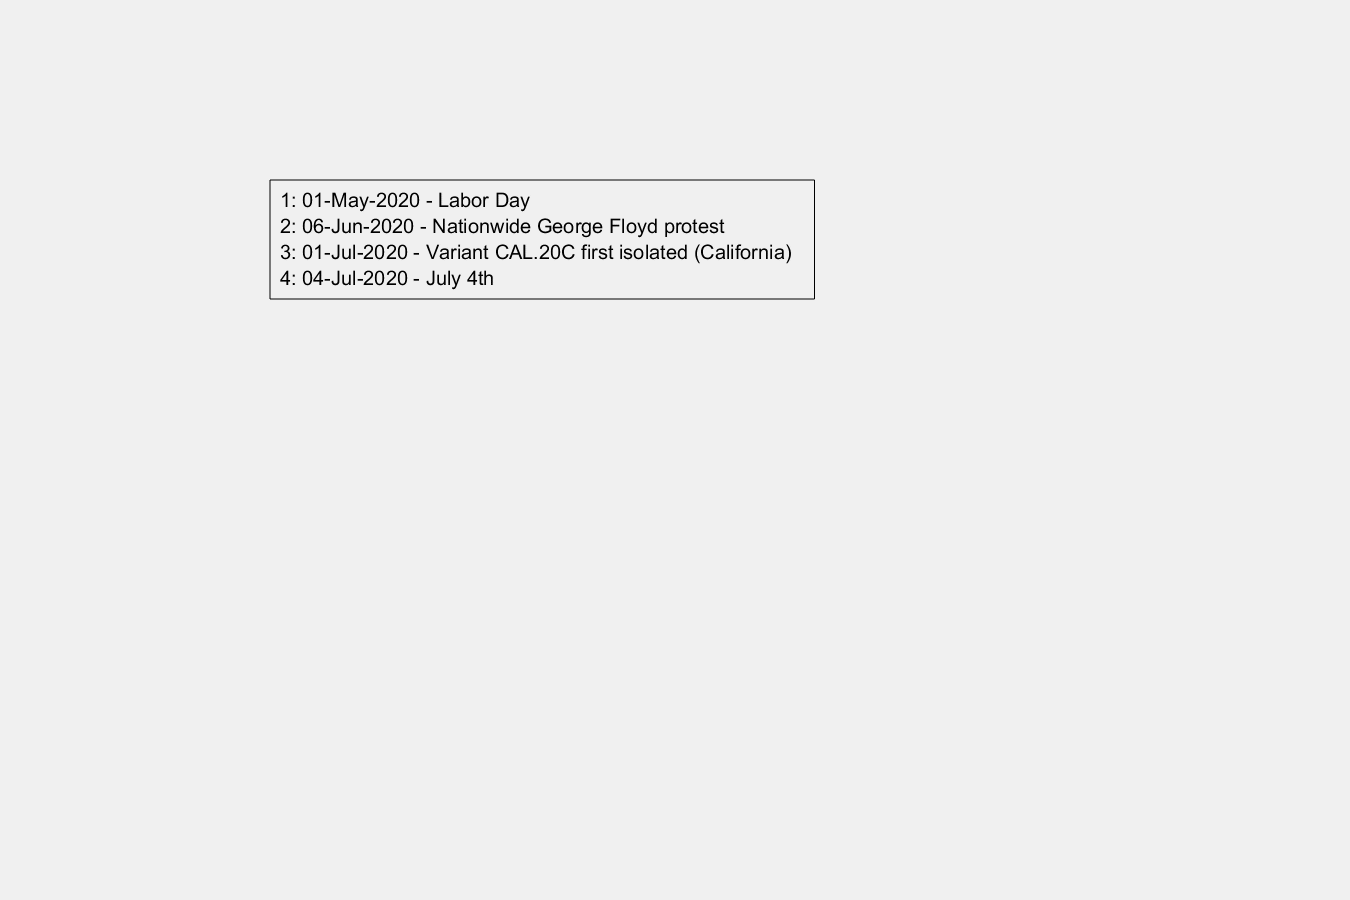
\includegraphics[width=\linewidth]{legends/CAL20C_legend.png}
	\caption{}
	\label{fig:legends/CAL20C_legendLabel}
\end{figure}

\begin{figure}
	\centering
	\subfigure[]{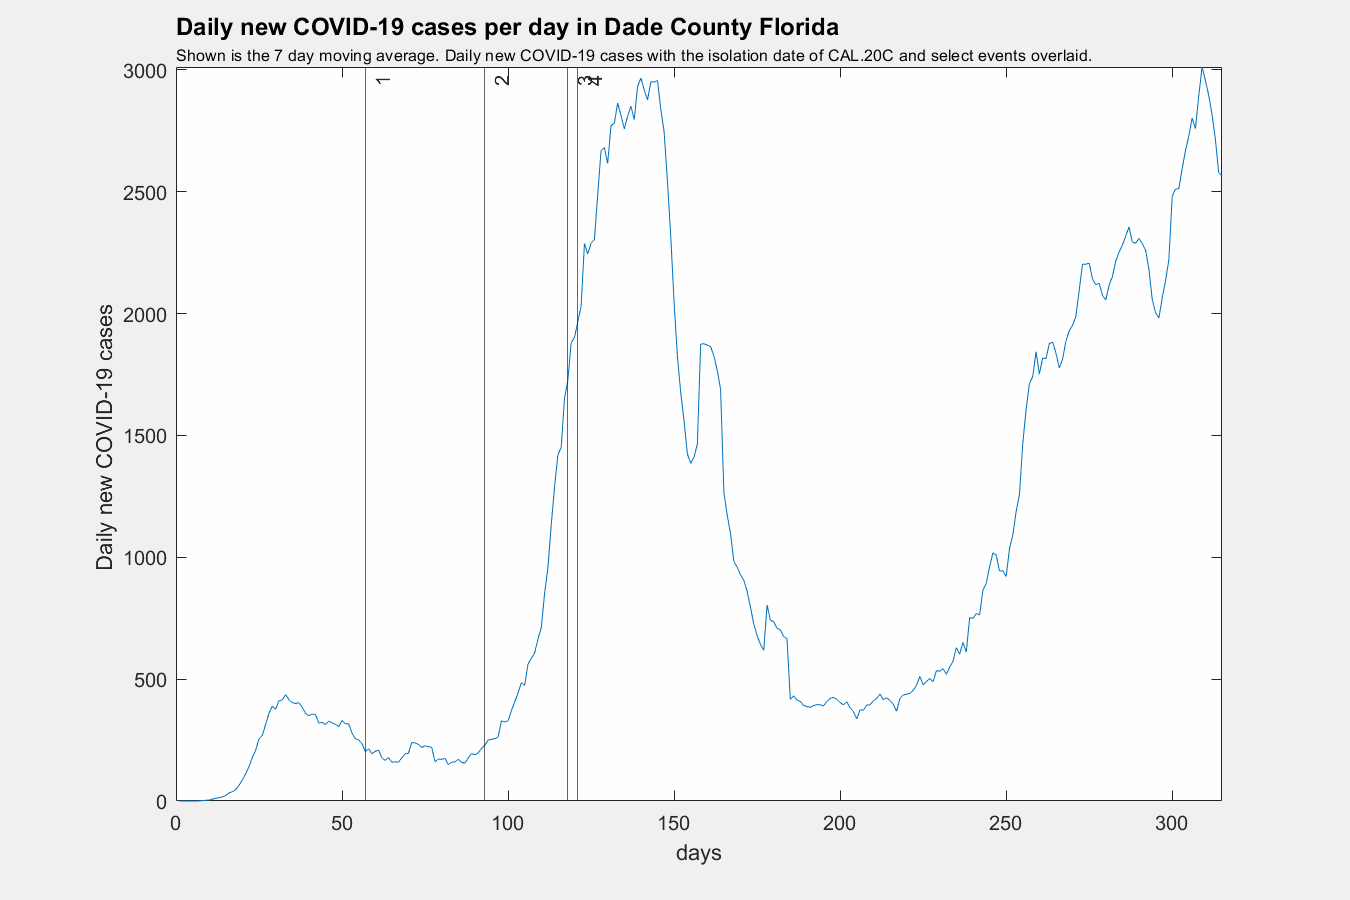
\includegraphics[width=0.26\textwidth]{images/dade_cases_CAL20C.png}}
	\subfigure[]{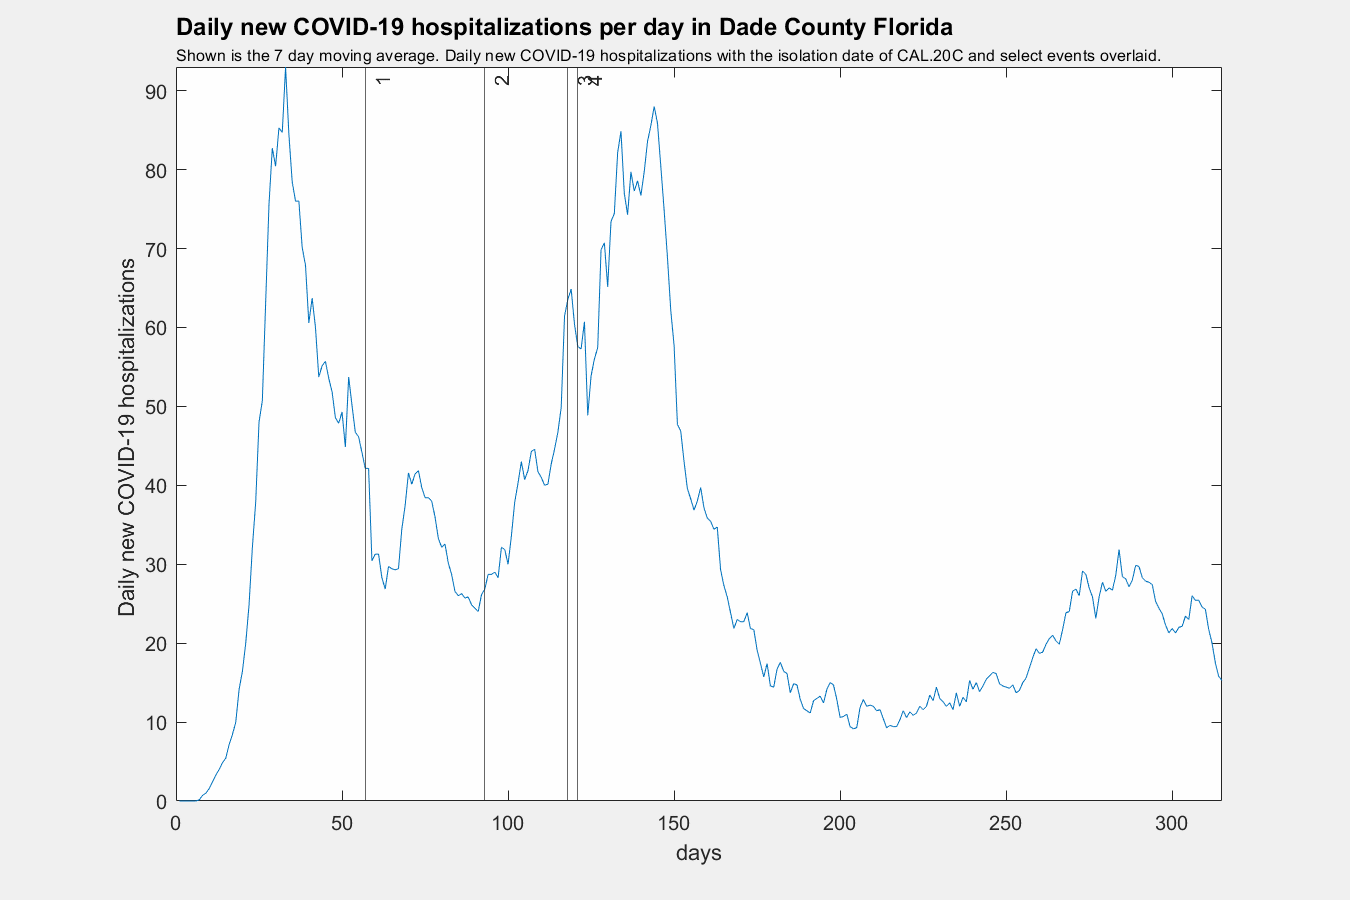
\includegraphics[width=0.26\textwidth]{images/dade_hospitalizations_CAL20C.png}}
	\subfigure[]{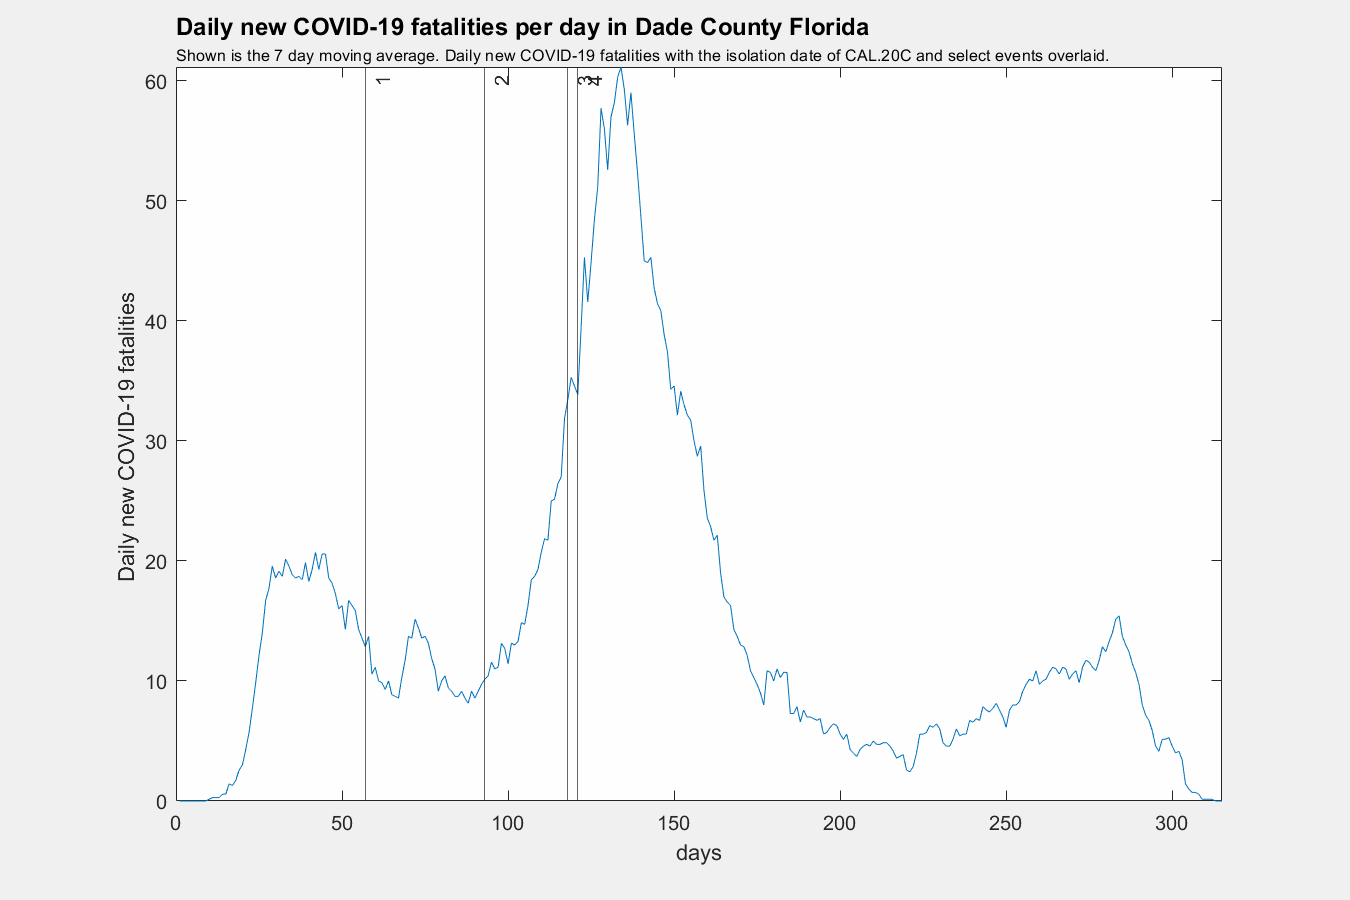
\includegraphics[width=0.26\textwidth]{images/dade_fatalities_CAL20C.png}}
	\subfigure[]{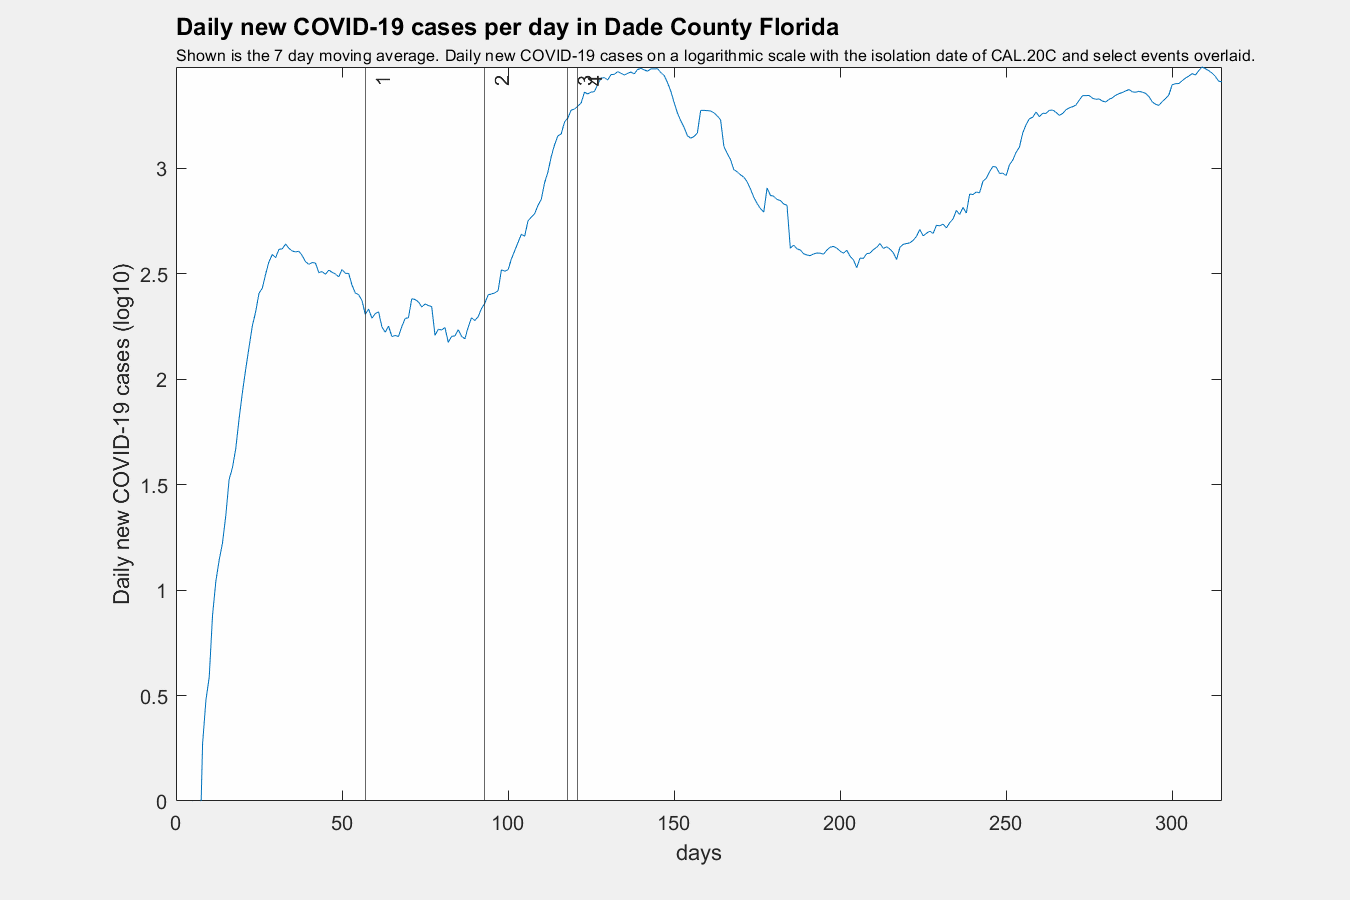
\includegraphics[width=0.26\textwidth]{images/dade_cases_CAL20C_log.png}}
	\subfigure[]{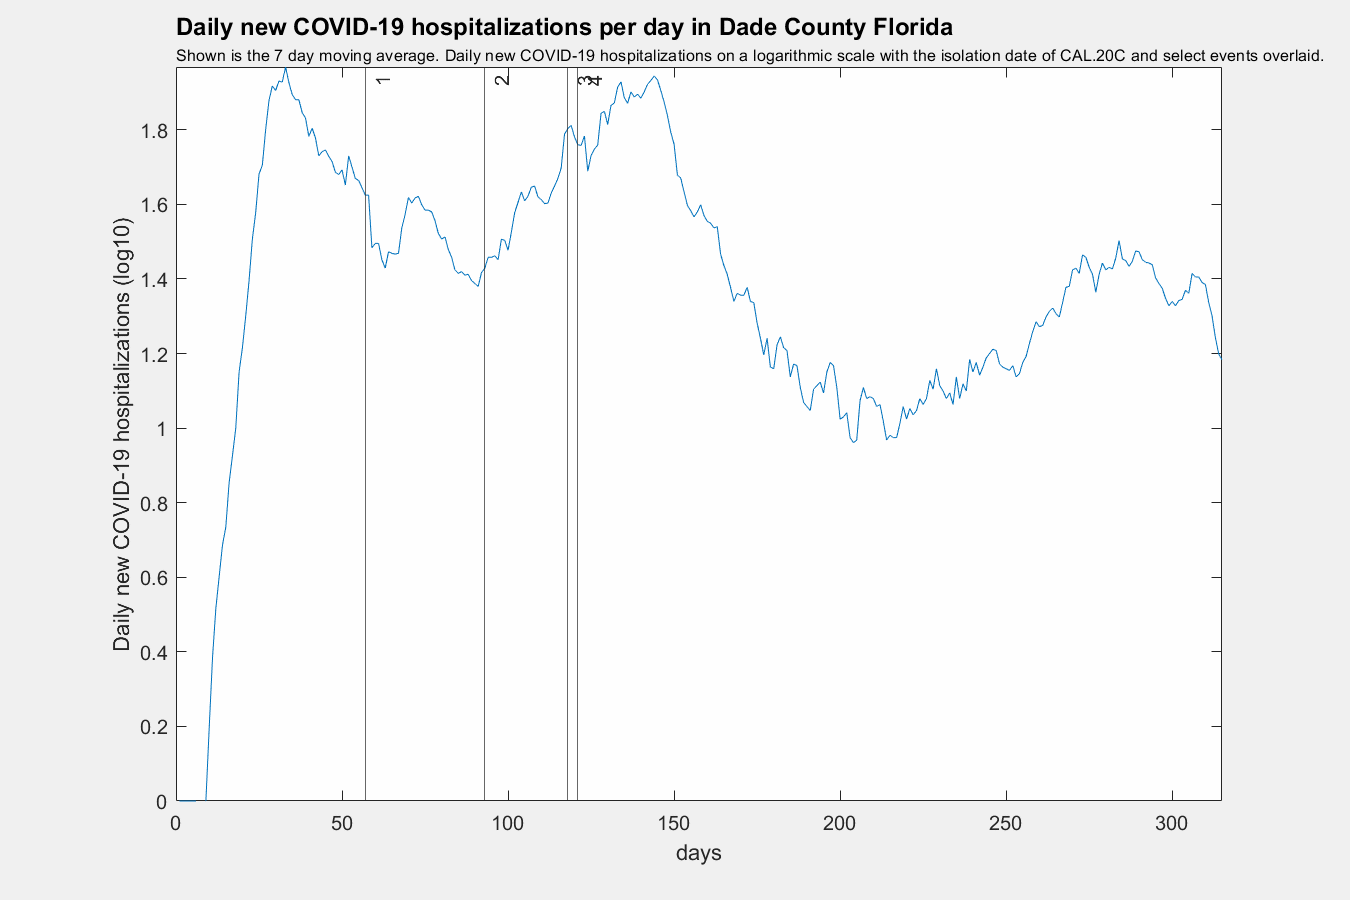
\includegraphics[width=0.26\textwidth]{images/dade_hospitalizations_CAL20C_log.png}}
	\subfigure[]{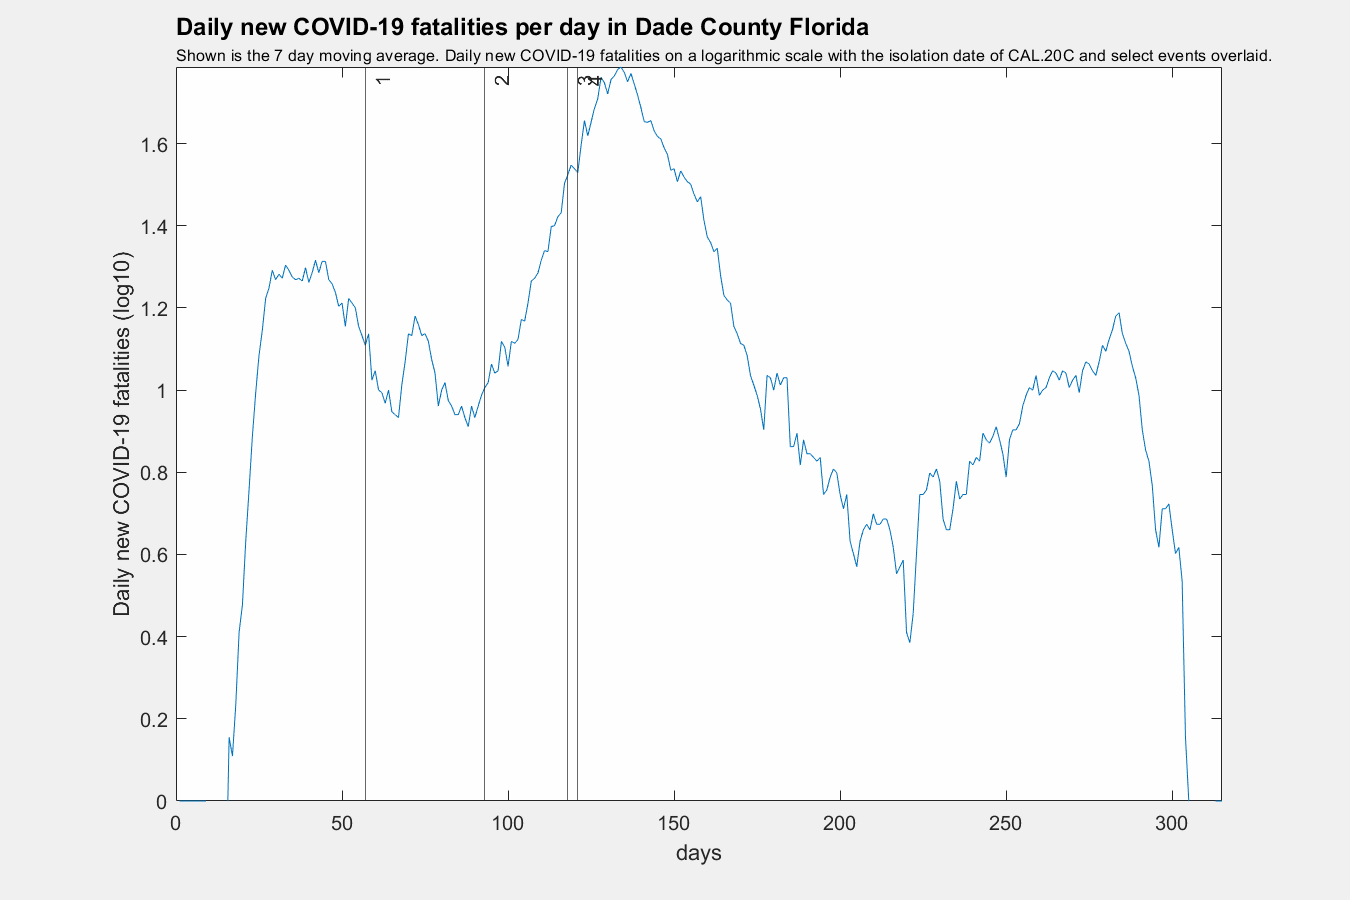
\includegraphics[width=0.26\textwidth]{images/dade_fatalities_CAL20C_log.png}}
	\subfigure[]{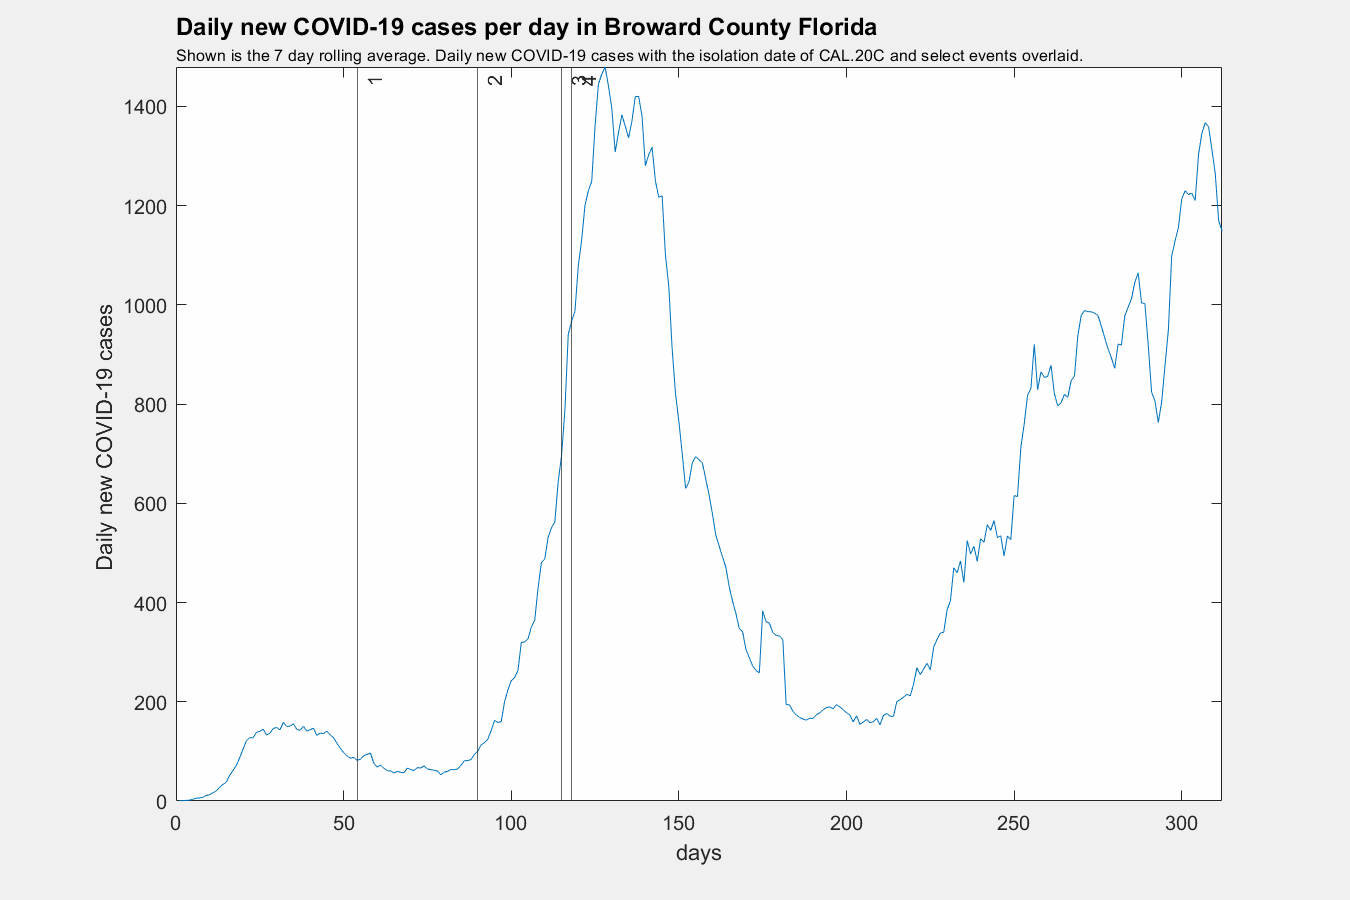
\includegraphics[width=0.26\textwidth]{images/broward_cases_CAL20C.png}}
	\subfigure[]{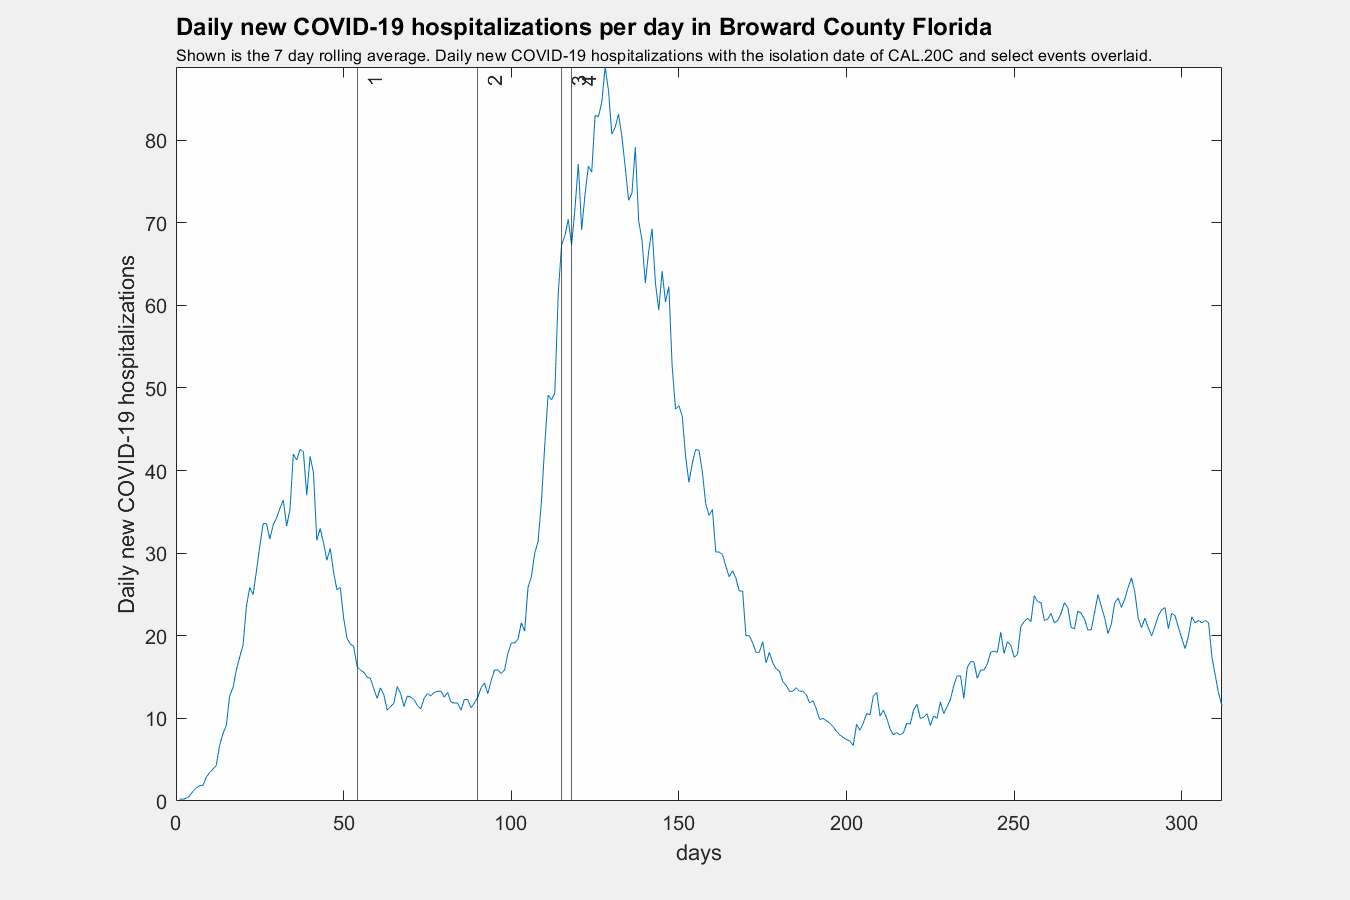
\includegraphics[width=0.26\textwidth]{images/broward_hospitalizations_CAL20C.png}}
	\subfigure[]{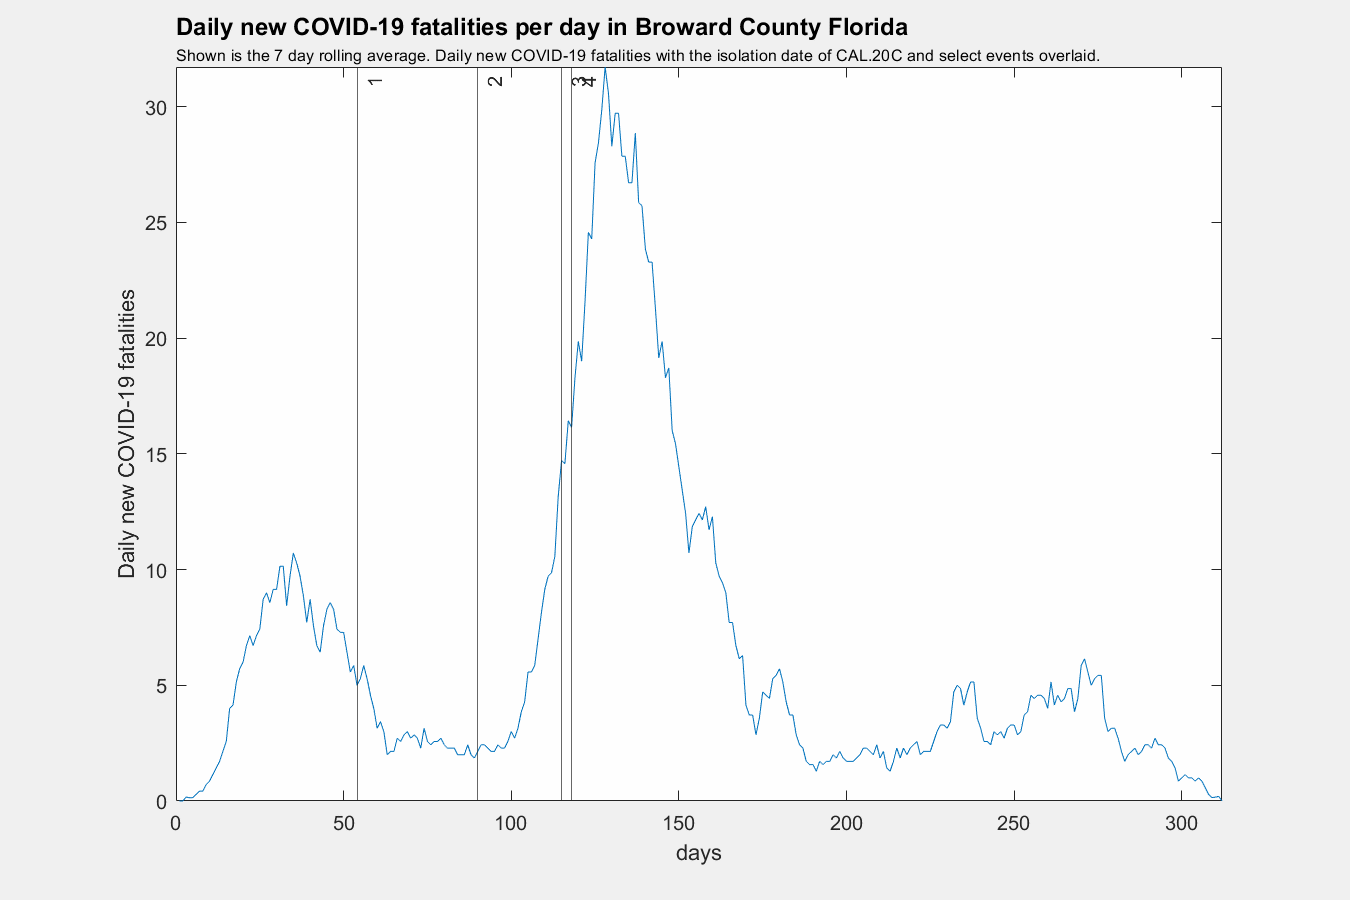
\includegraphics[width=0.26\textwidth]{images/broward_fatalities_CAL20C.png}}
	\subfigure[]{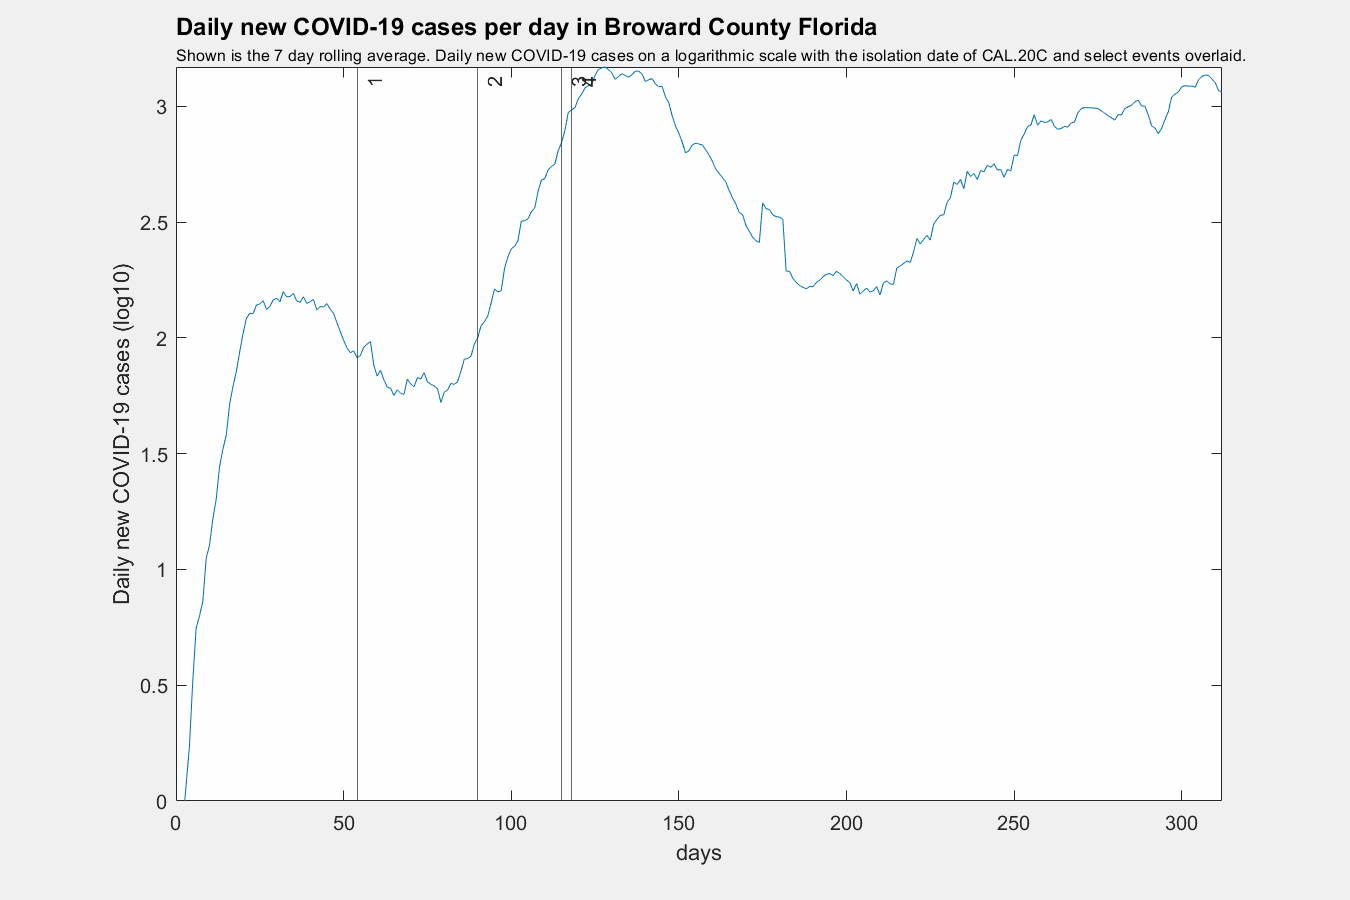
\includegraphics[width=0.26\textwidth]{images/broward_cases_CAL20C_log.png}}
	\subfigure[]{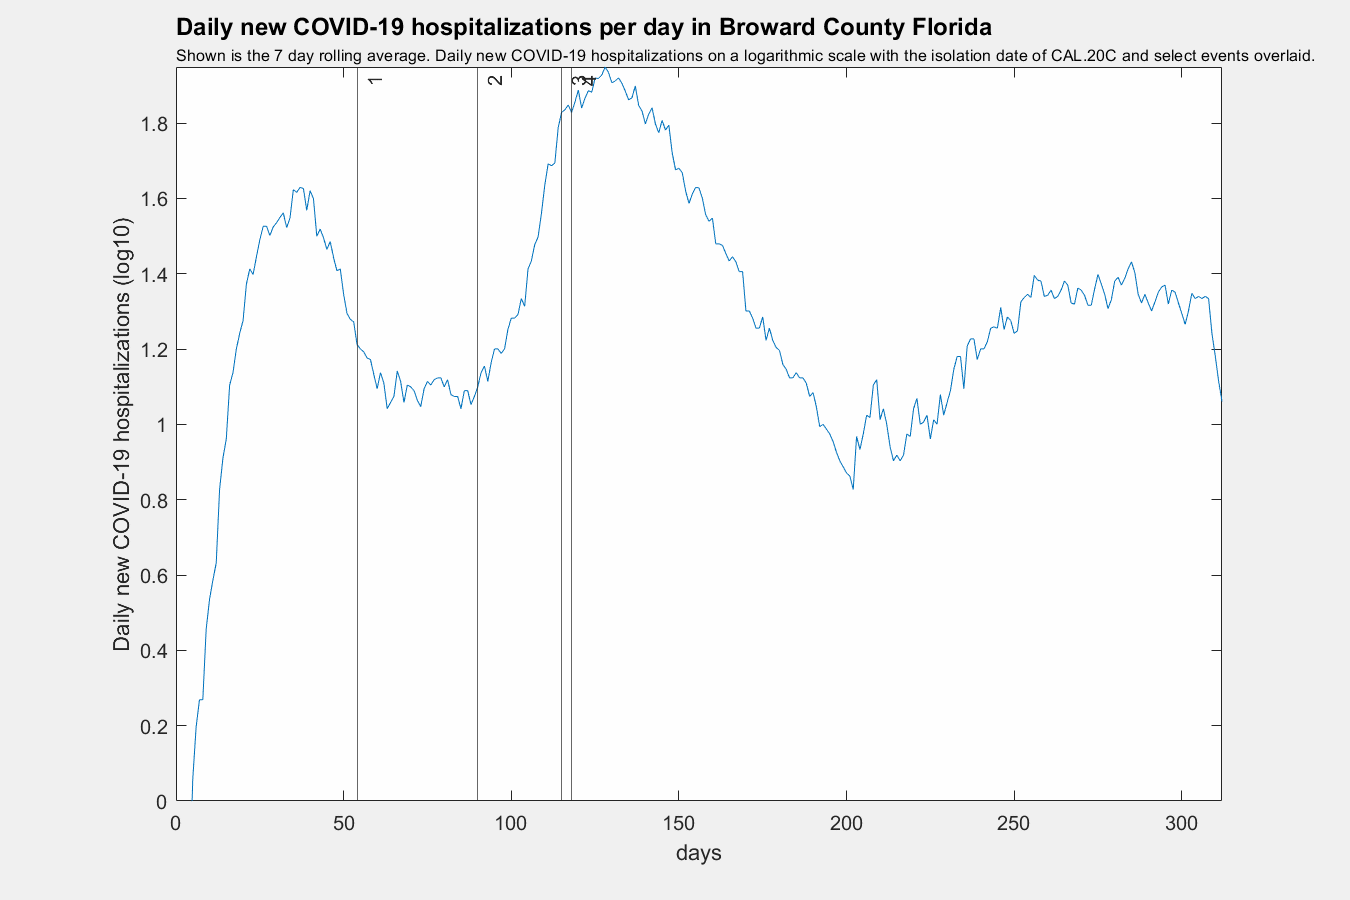
\includegraphics[width=0.26\textwidth]{images/broward_hospitalizations_CAL20C_log.png}}
	\subfigure[]{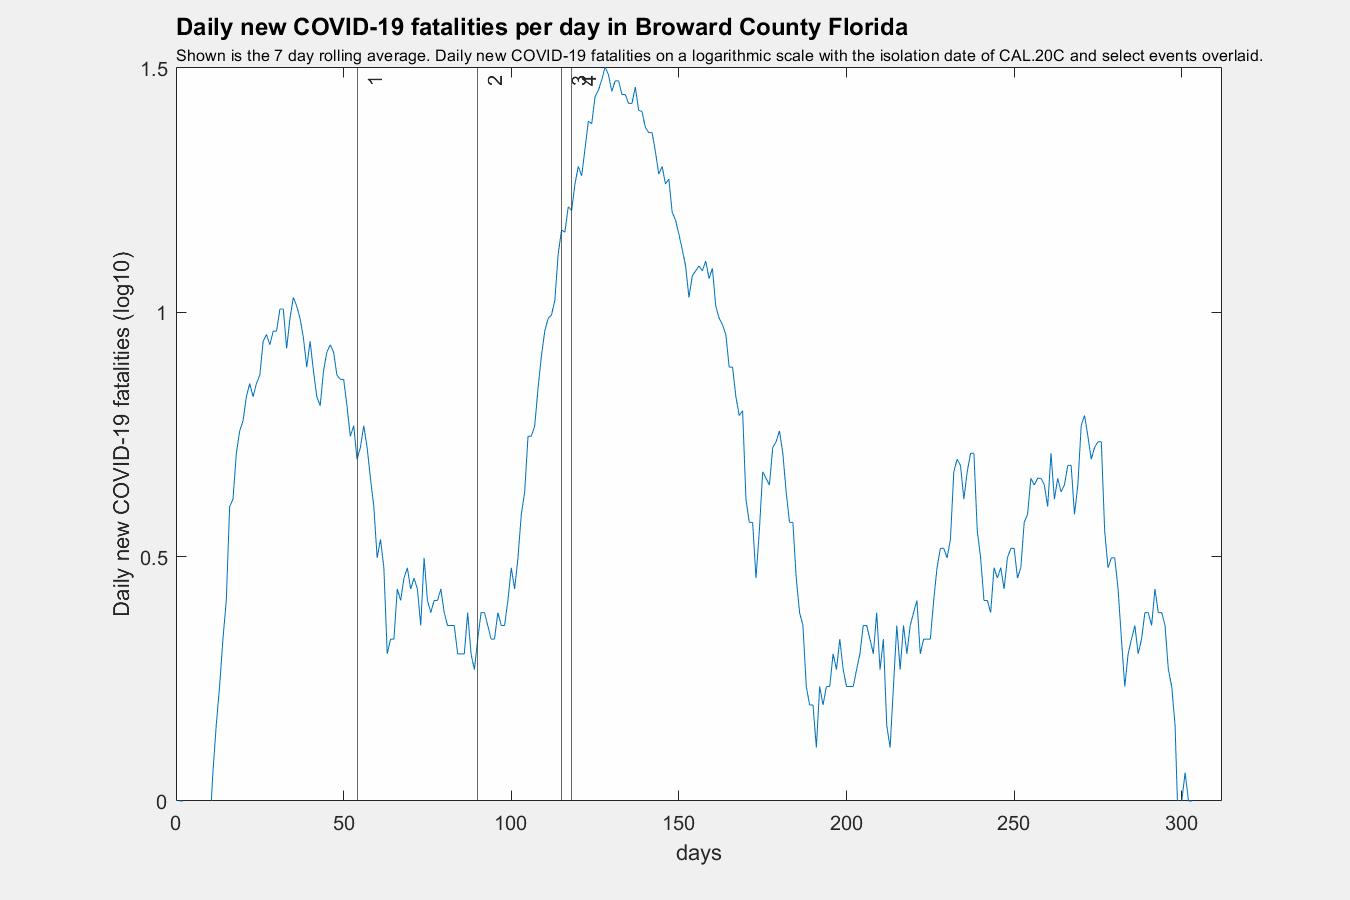
\includegraphics[width=0.26\textwidth]{images/broward_fatalities_CAL20C_log.png}}
	\subfigure[]{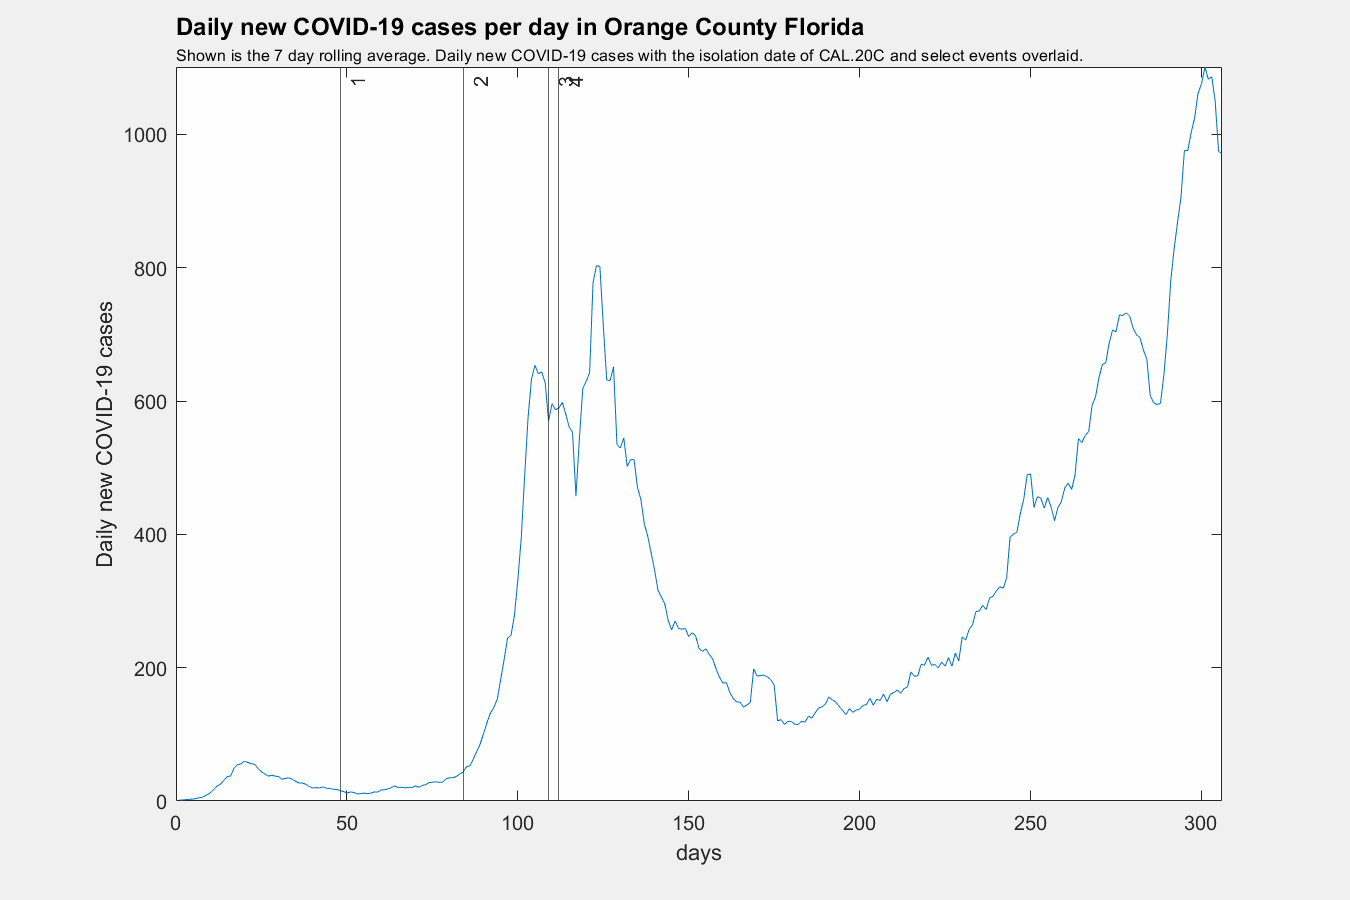
\includegraphics[width=0.26\textwidth]{images/orange_cases_CAL20C.png}}
	\subfigure[]{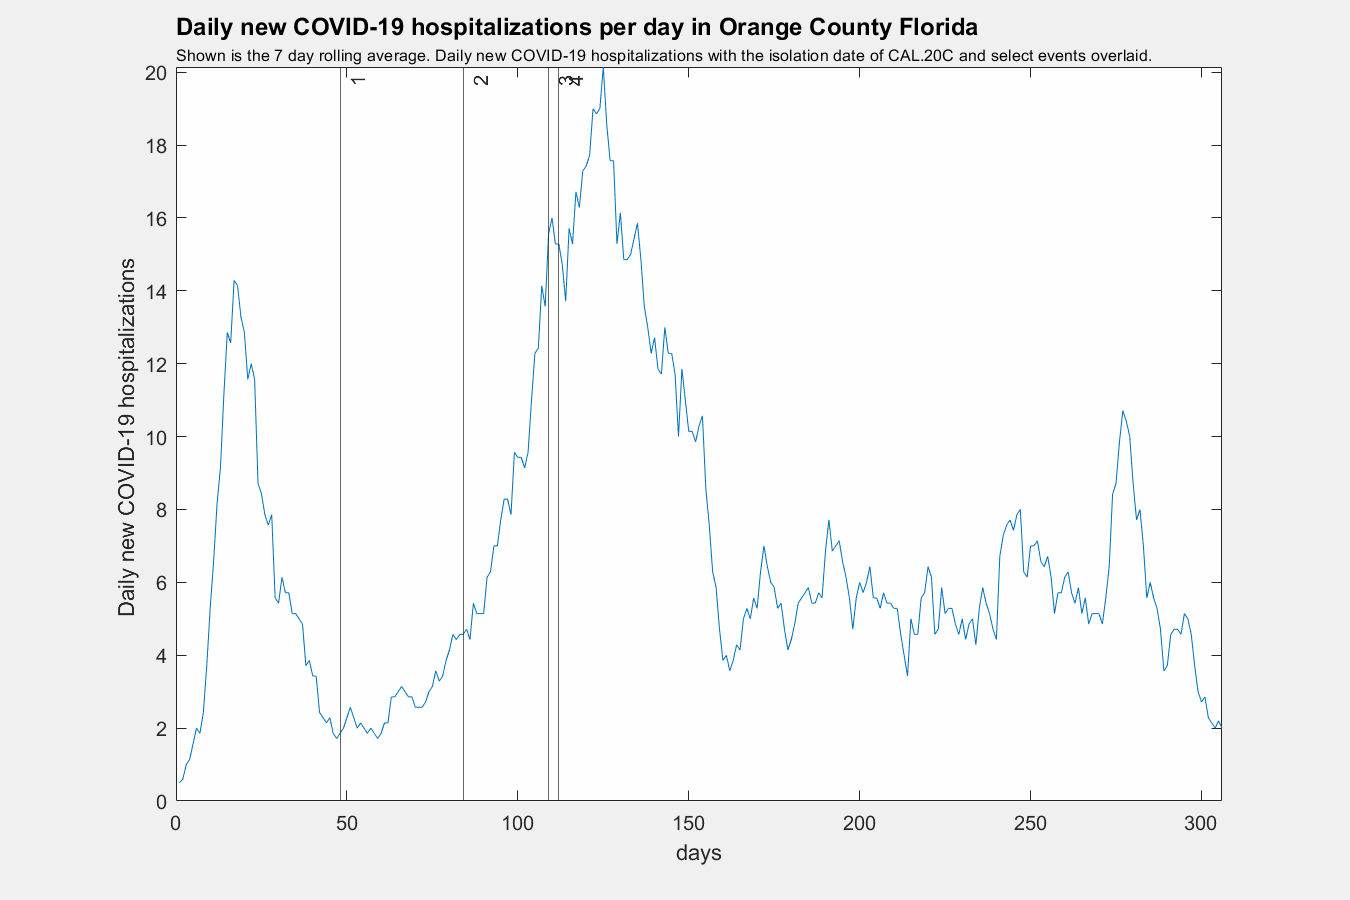
\includegraphics[width=0.26\textwidth]{images/orange_hospitalizations_CAL20C.png}}
	\subfigure[]{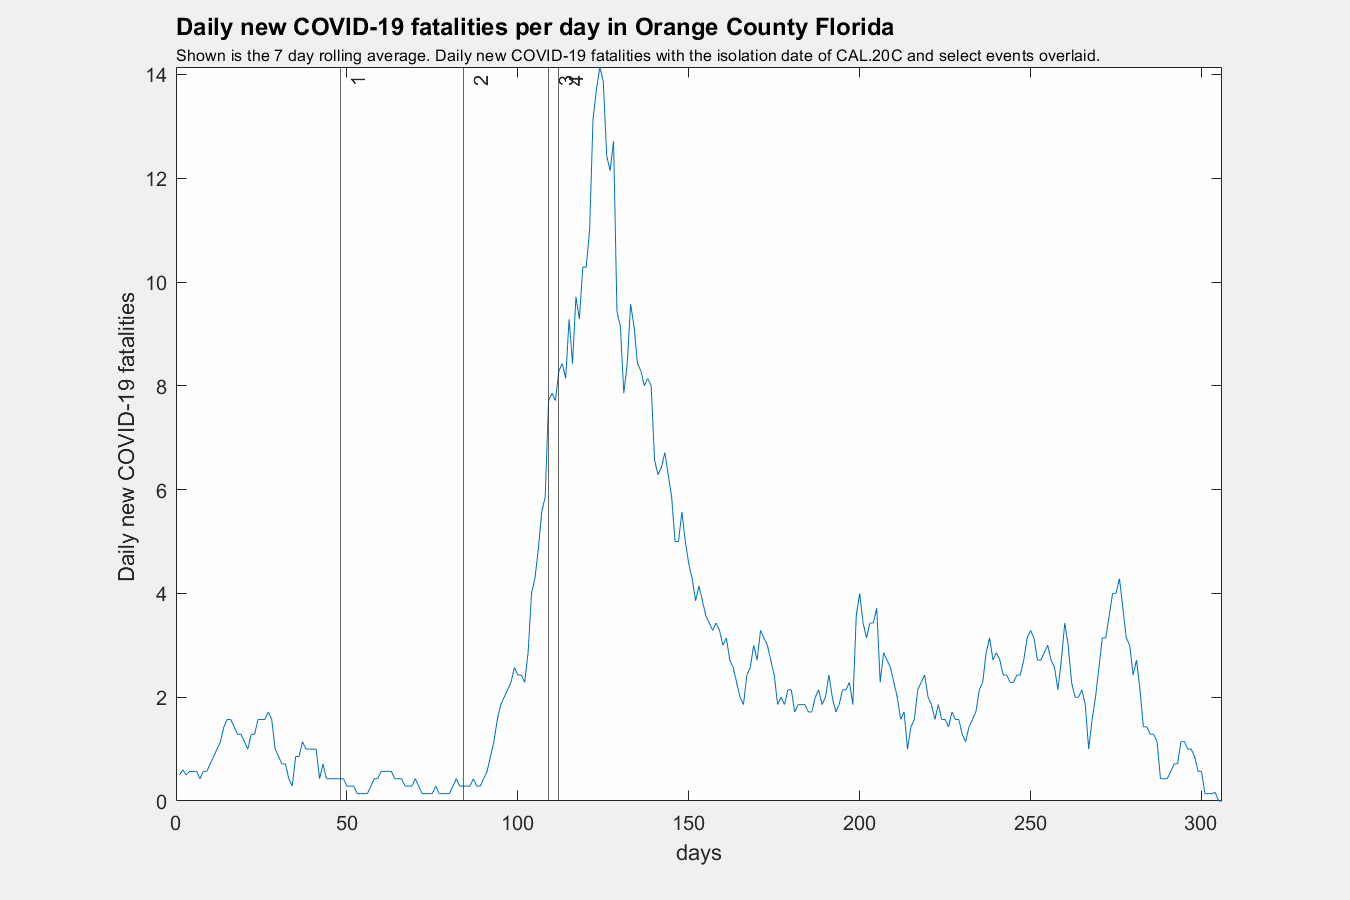
\includegraphics[width=0.26\textwidth]{images/orange_fatalities_CAL20C.png}}
	\subfigure[]{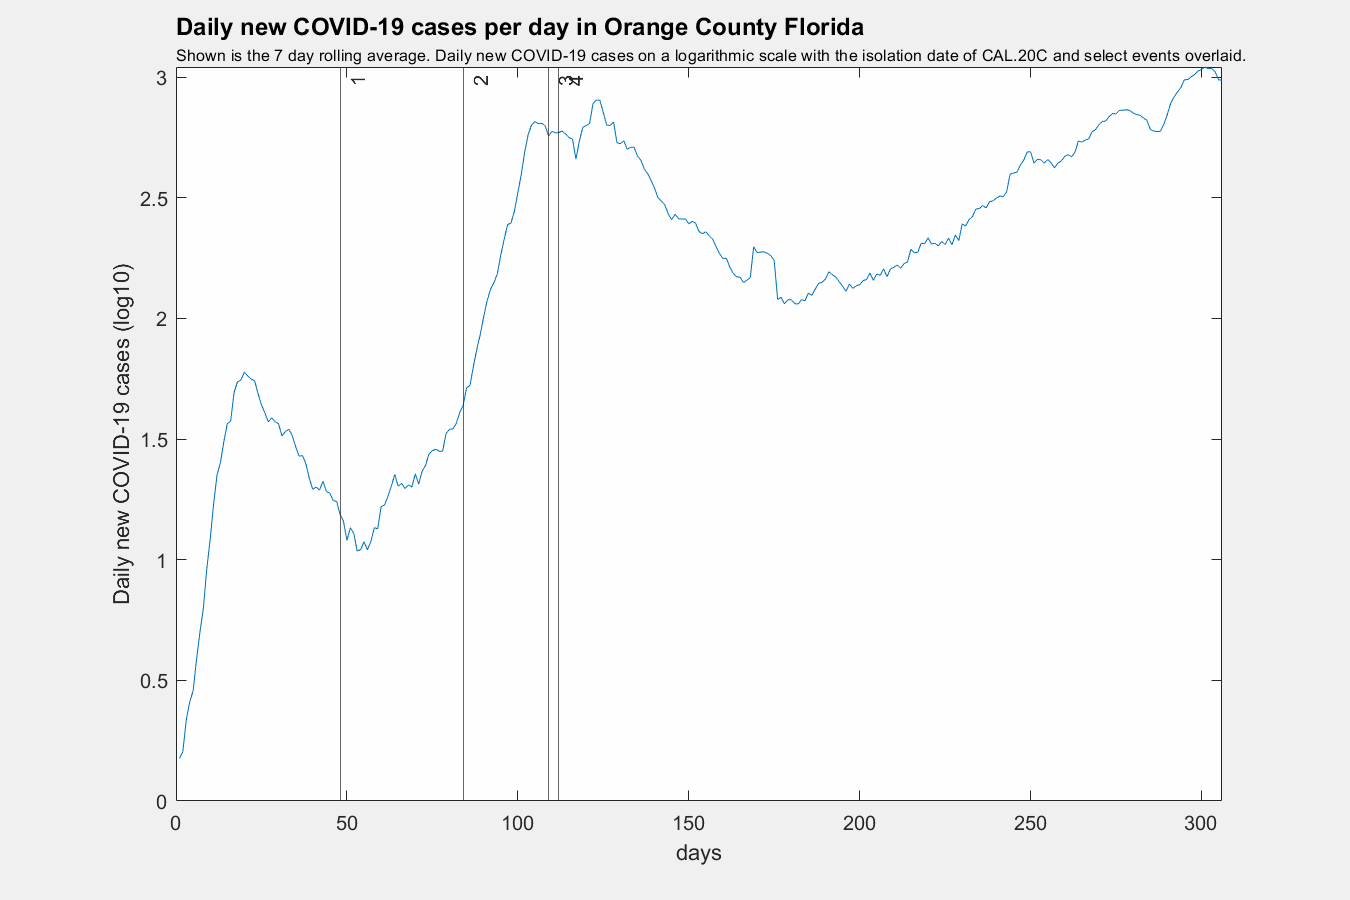
\includegraphics[width=0.26\textwidth]{images/orange_cases_CAL20C_log.png}}
	\subfigure[]{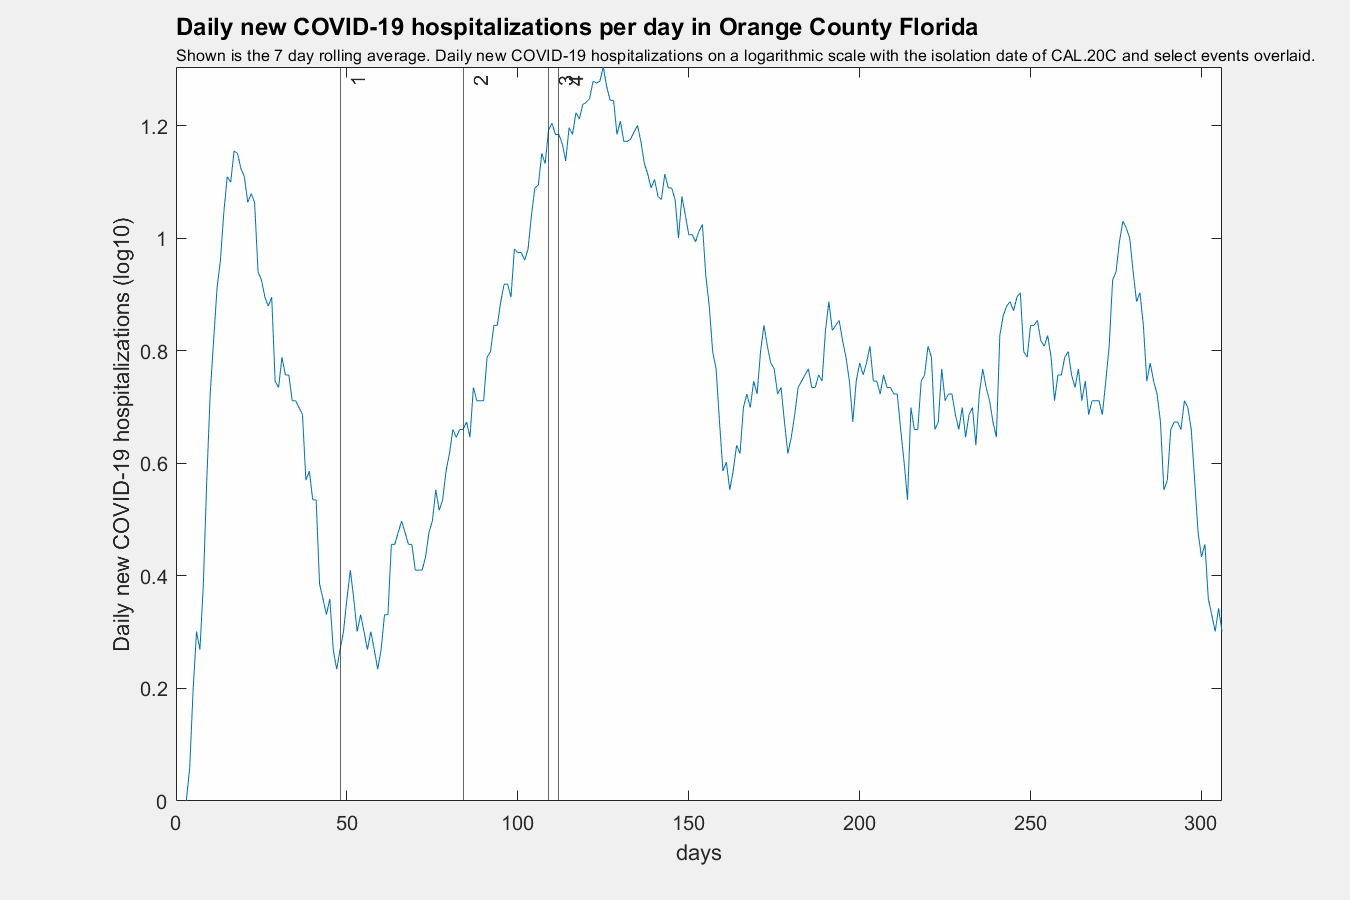
\includegraphics[width=0.26\textwidth]{images/orange_hospitalizations_CAL20C_log.png}}
	\subfigure[]{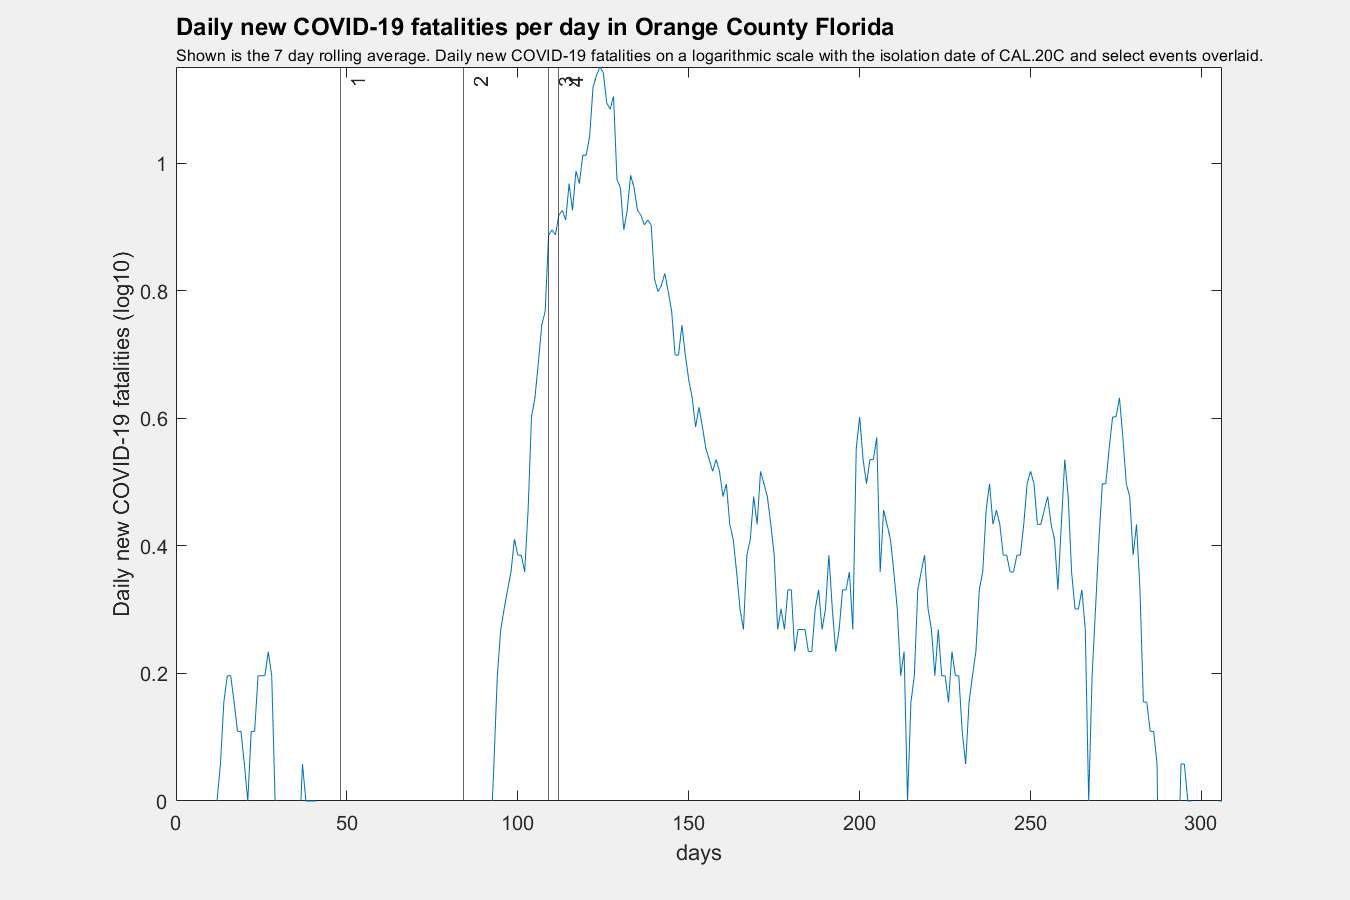
\includegraphics[width=0.26\textwidth]{images/orange_fatalities_CAL20C_log.png}}
	\caption{(a-f) Dade County; (g-l) Broward County; (m-r) Orange County }
	\label{fig:foobar}
\end{figure}
\FloatBarrier
\vspace{5mm}

\subsection{California}

\begin{figure}[!h]
	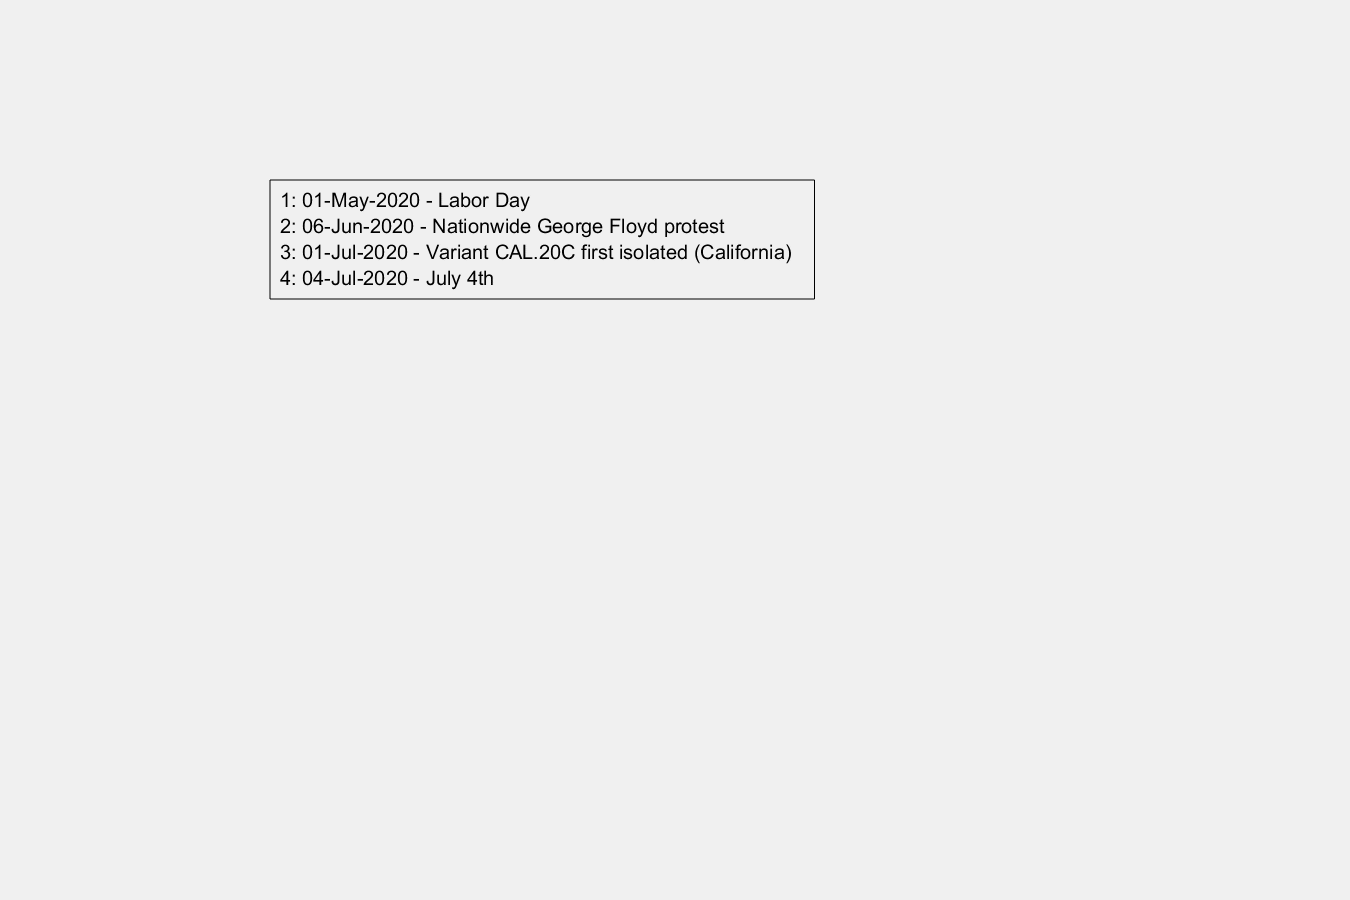
\includegraphics[width=\linewidth]{legends/CAL20C_legend.png}
	\caption{}
	\label{fig:legends/CAL20C_legendLabel}
\end{figure}

\begin{figure}
	\centering
	\subfigure[]{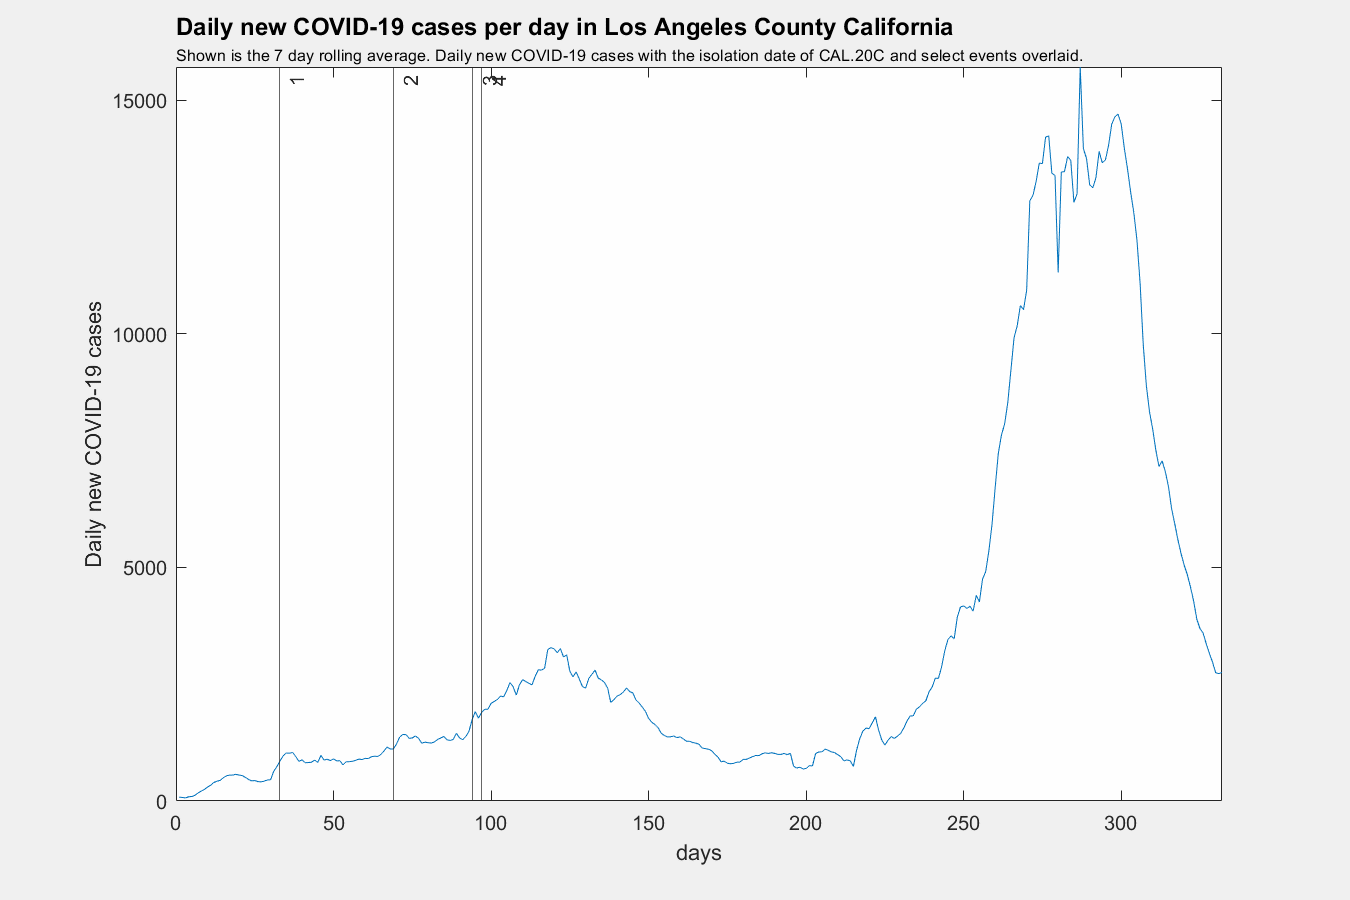
\includegraphics[width=0.26\textwidth]{images/los_angeles_cases_CAL20C.png}}
	\subfigure[]{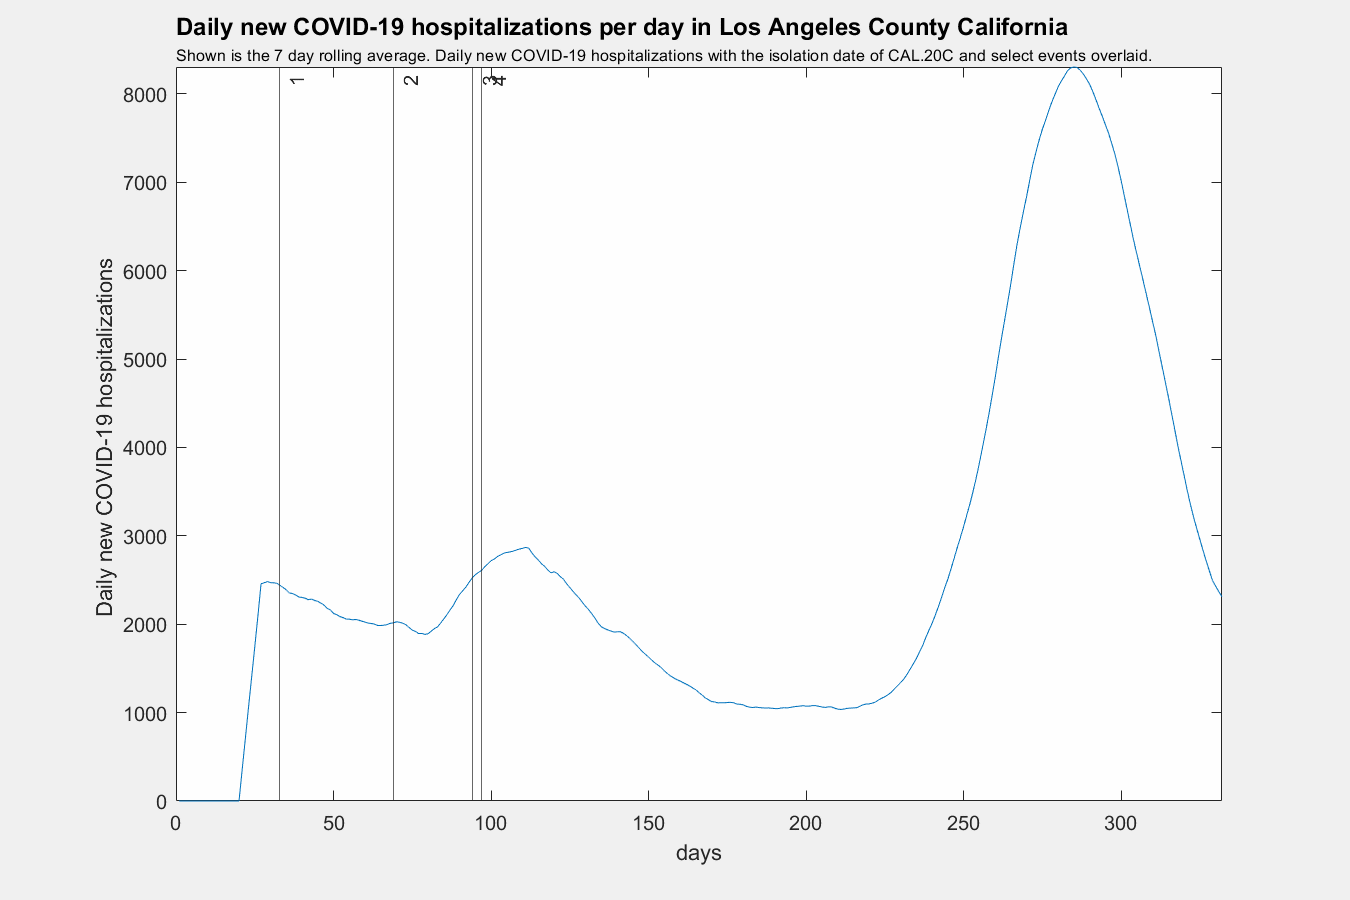
\includegraphics[width=0.26\textwidth]{images/los_angeles_hospitalizations_CAL20C.png}}
	\subfigure[]{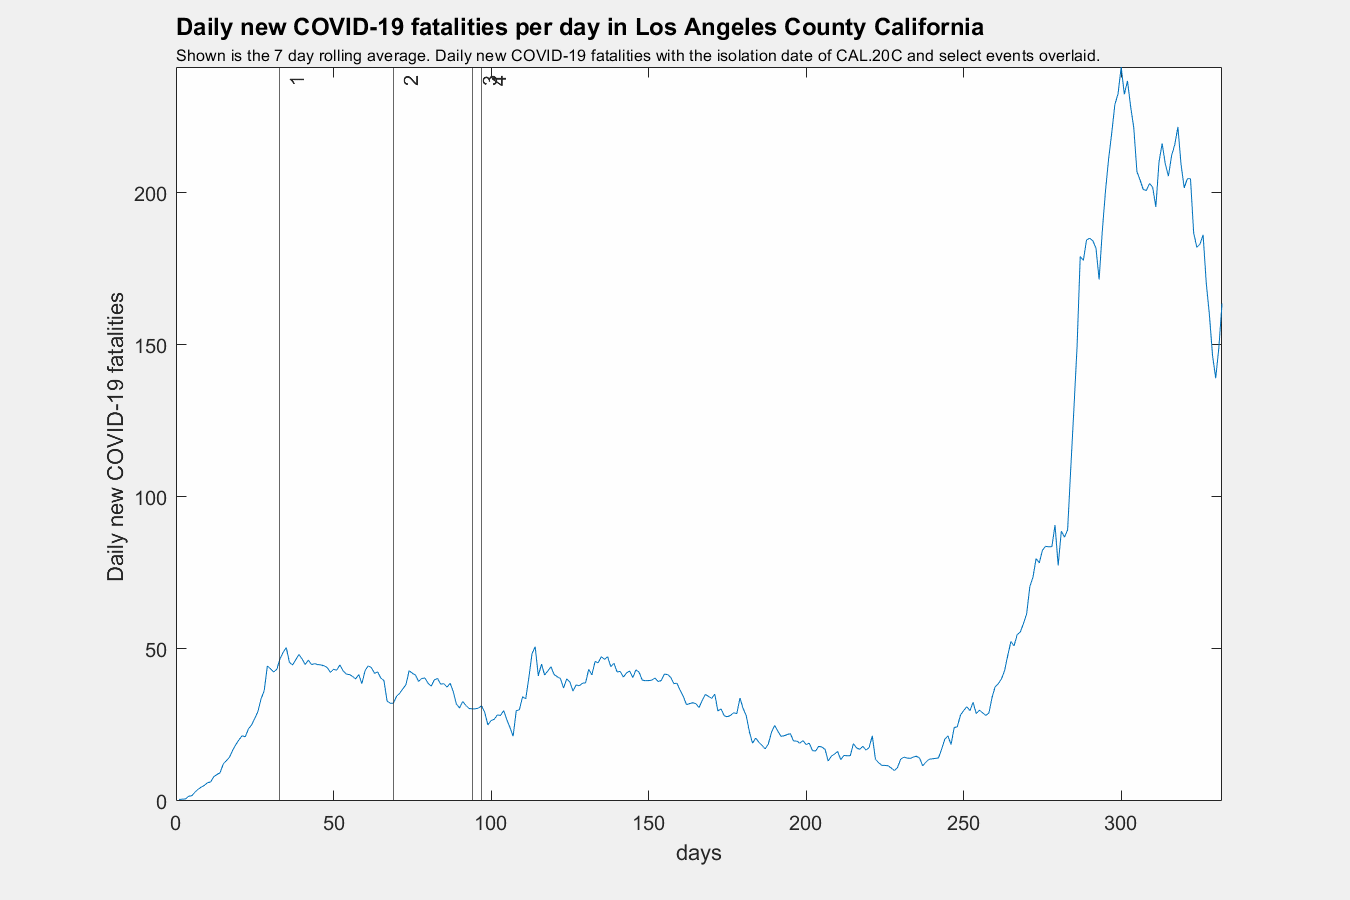
\includegraphics[width=0.26\textwidth]{images/los_angeles_fatalities_CAL20C.png}}
	\subfigure[]{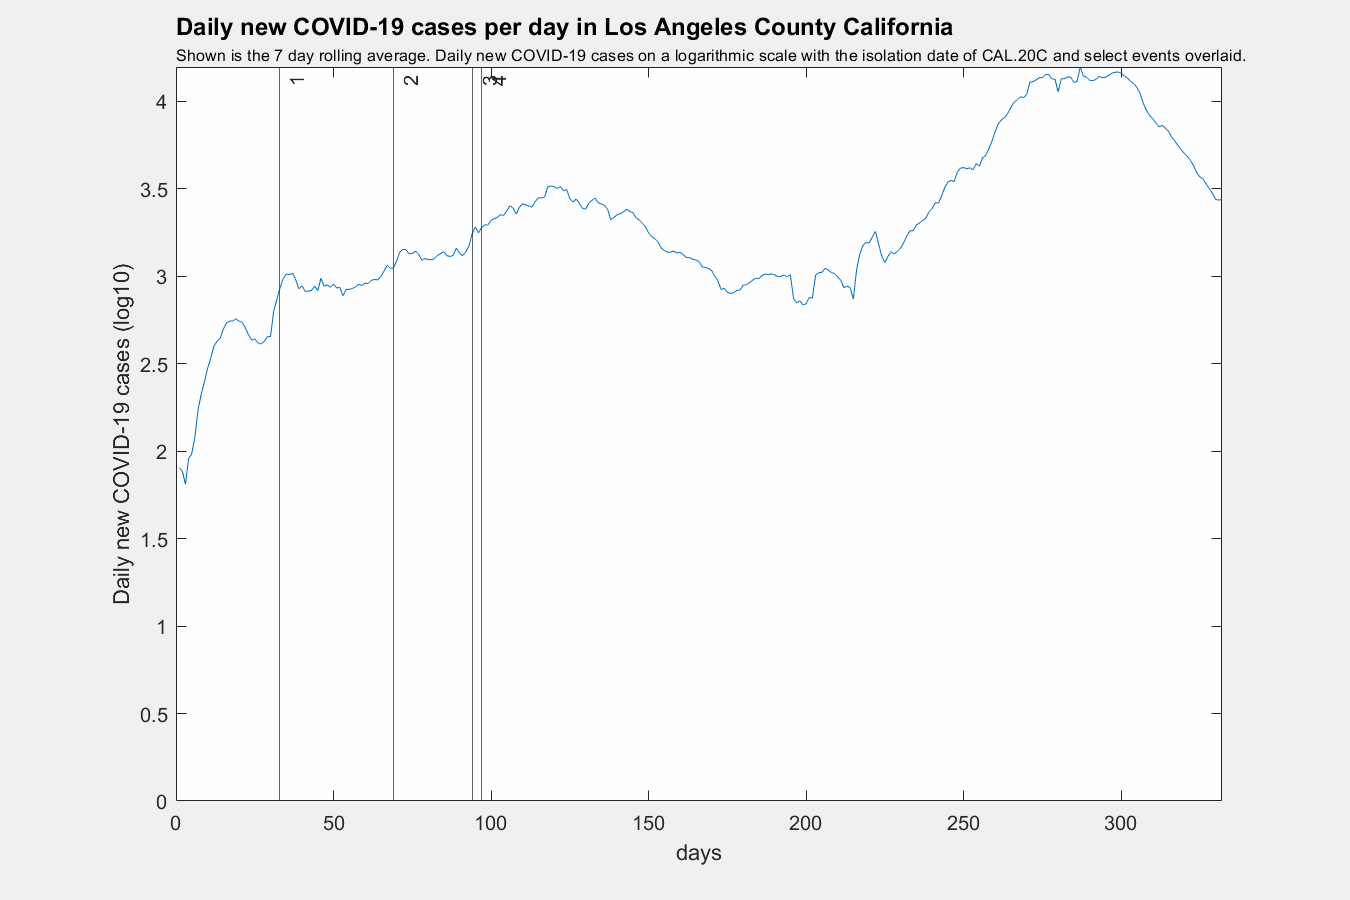
\includegraphics[width=0.26\textwidth]{images/los_angeles_cases_CAL20C_log.png}}
	\subfigure[]{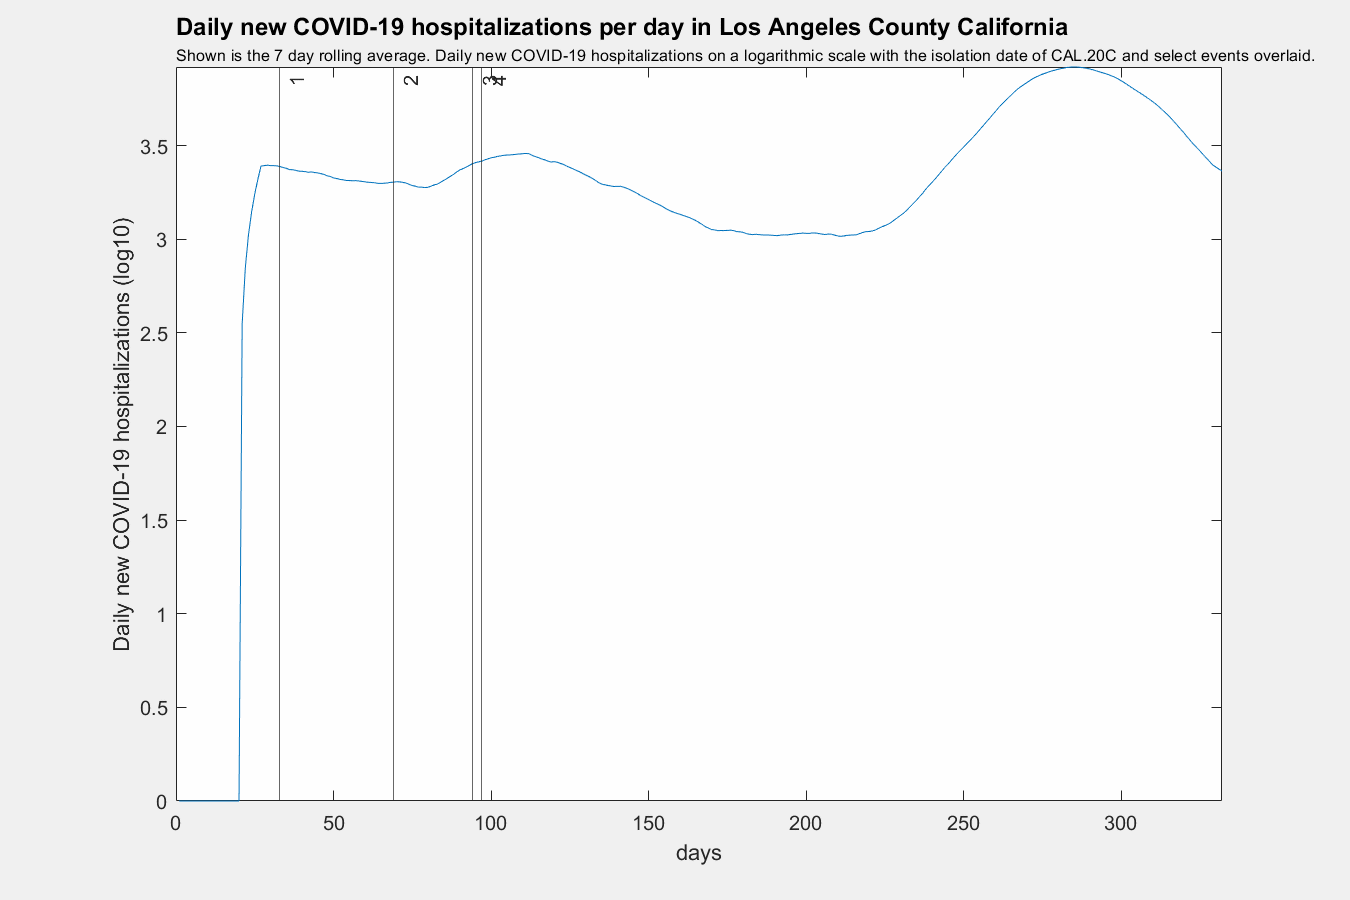
\includegraphics[width=0.26\textwidth]{images/los_angeles_hospitalizations_CAL20C_log.png}}
	\subfigure[]{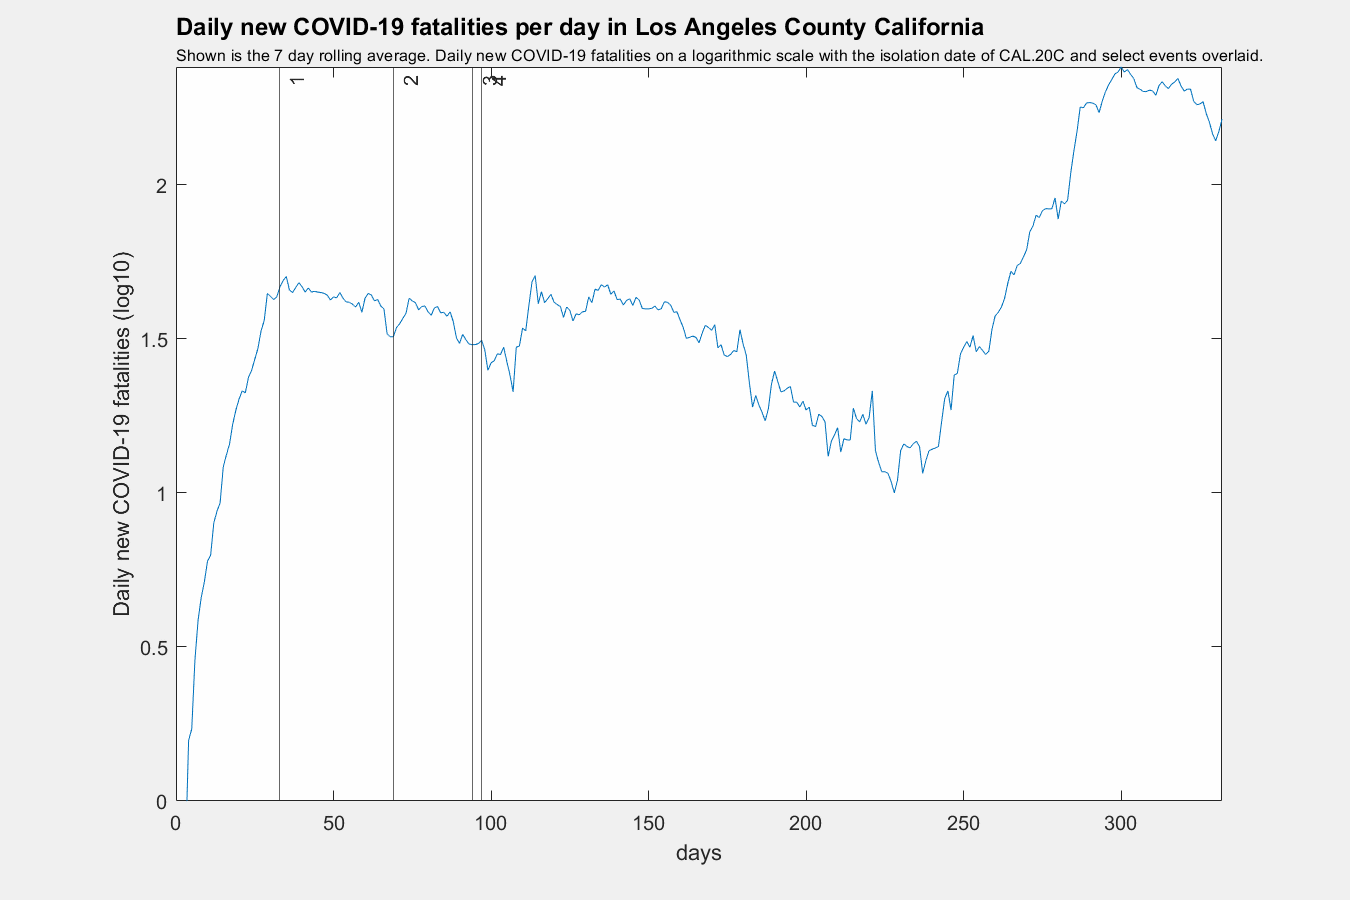
\includegraphics[width=0.26\textwidth]{images/los_angeles_fatalities_CAL20C_log.png}}
	\subfigure[]{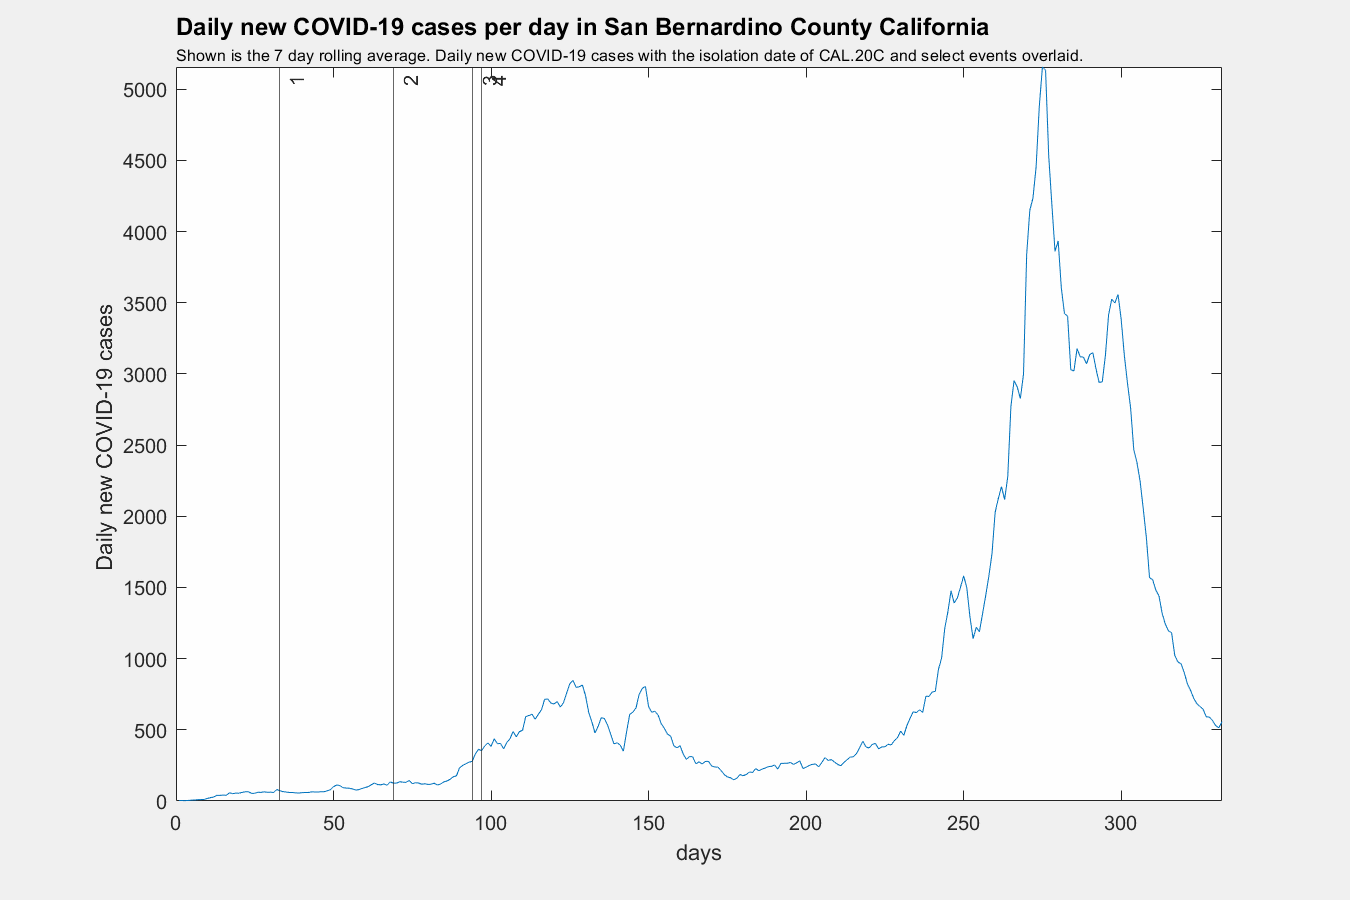
\includegraphics[width=0.26\textwidth]{images/san_bernardino_cases_CAL20C.png}}
	\subfigure[]{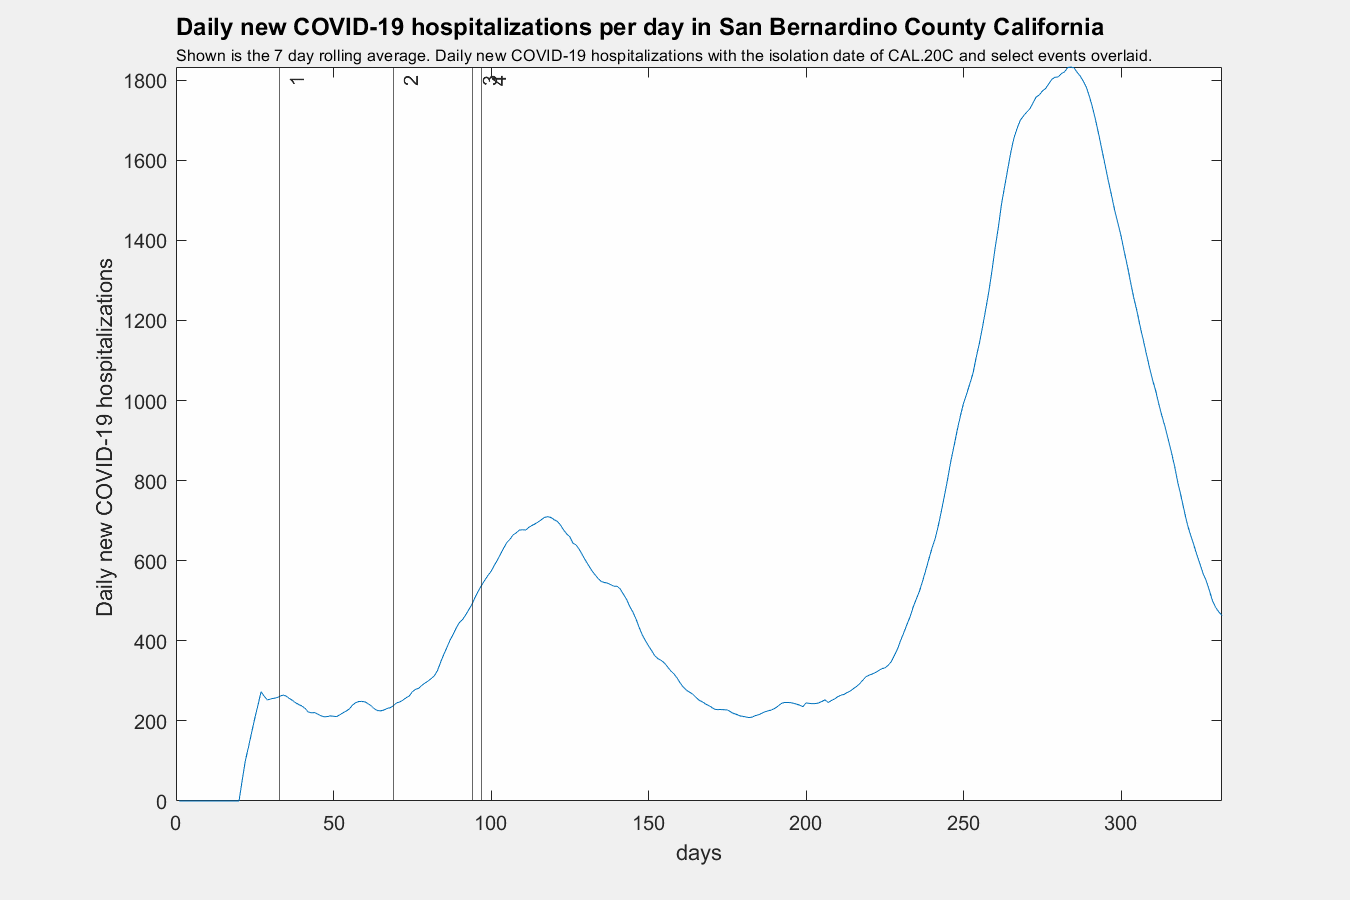
\includegraphics[width=0.26\textwidth]{images/san_bernardino_hospitalizations_CAL20C.png}}
	\subfigure[]{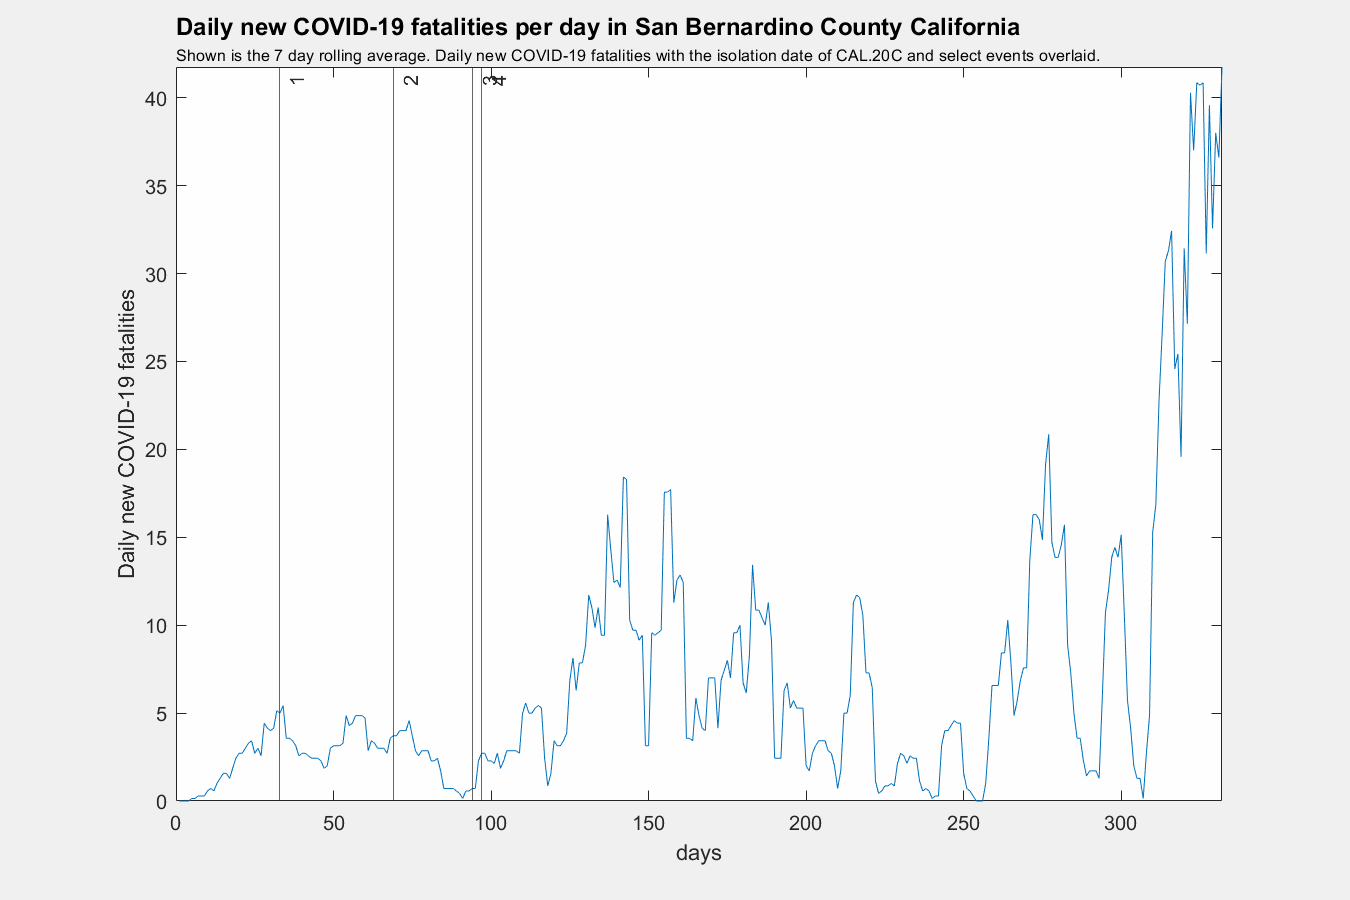
\includegraphics[width=0.26\textwidth]{images/san_bernardino_fatalities_CAL20C.png}}
	\subfigure[]{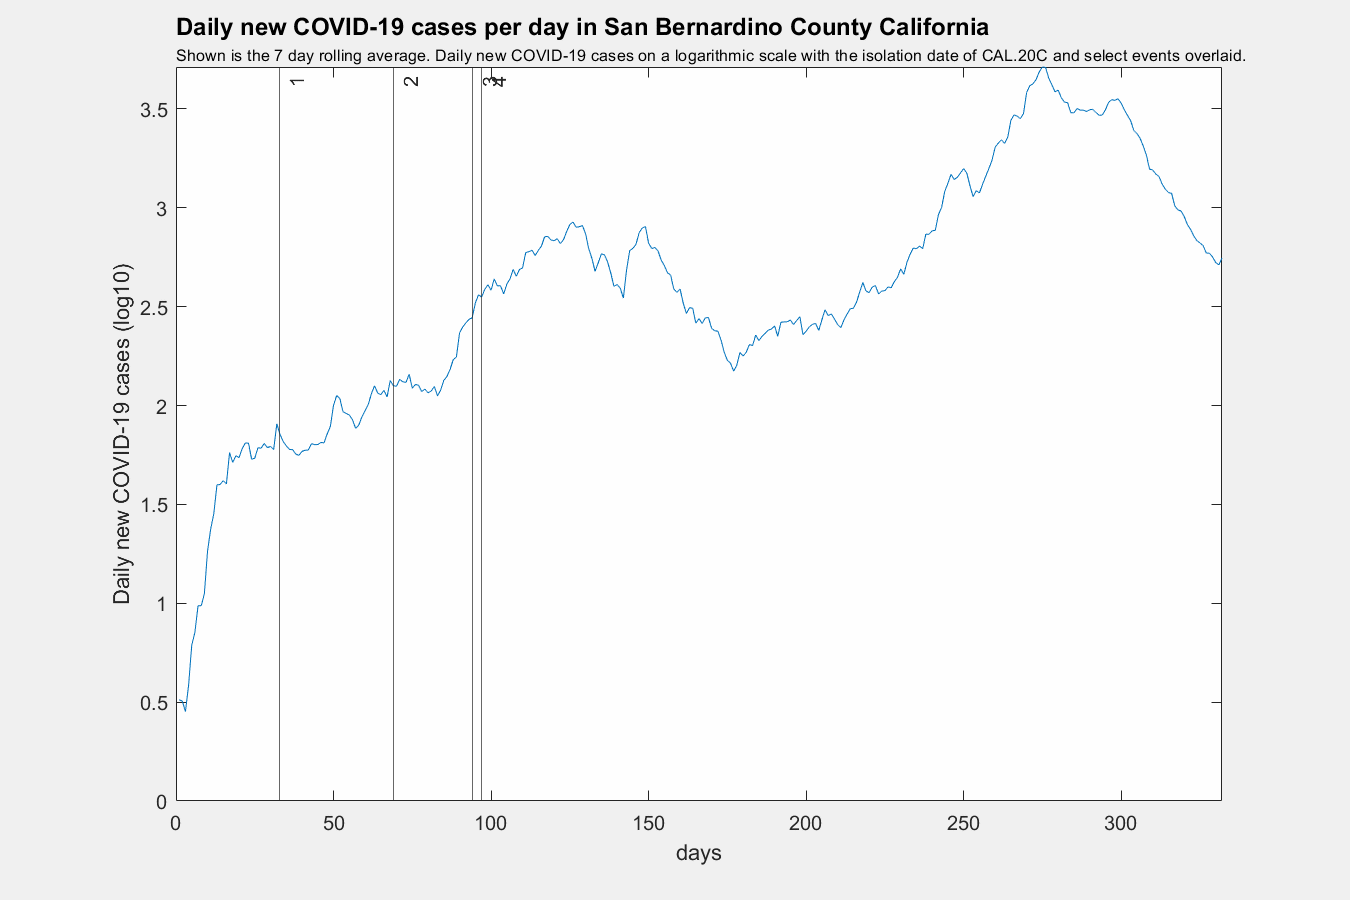
\includegraphics[width=0.26\textwidth]{images/san_bernardino_cases_CAL20C_log.png}}
	\subfigure[]{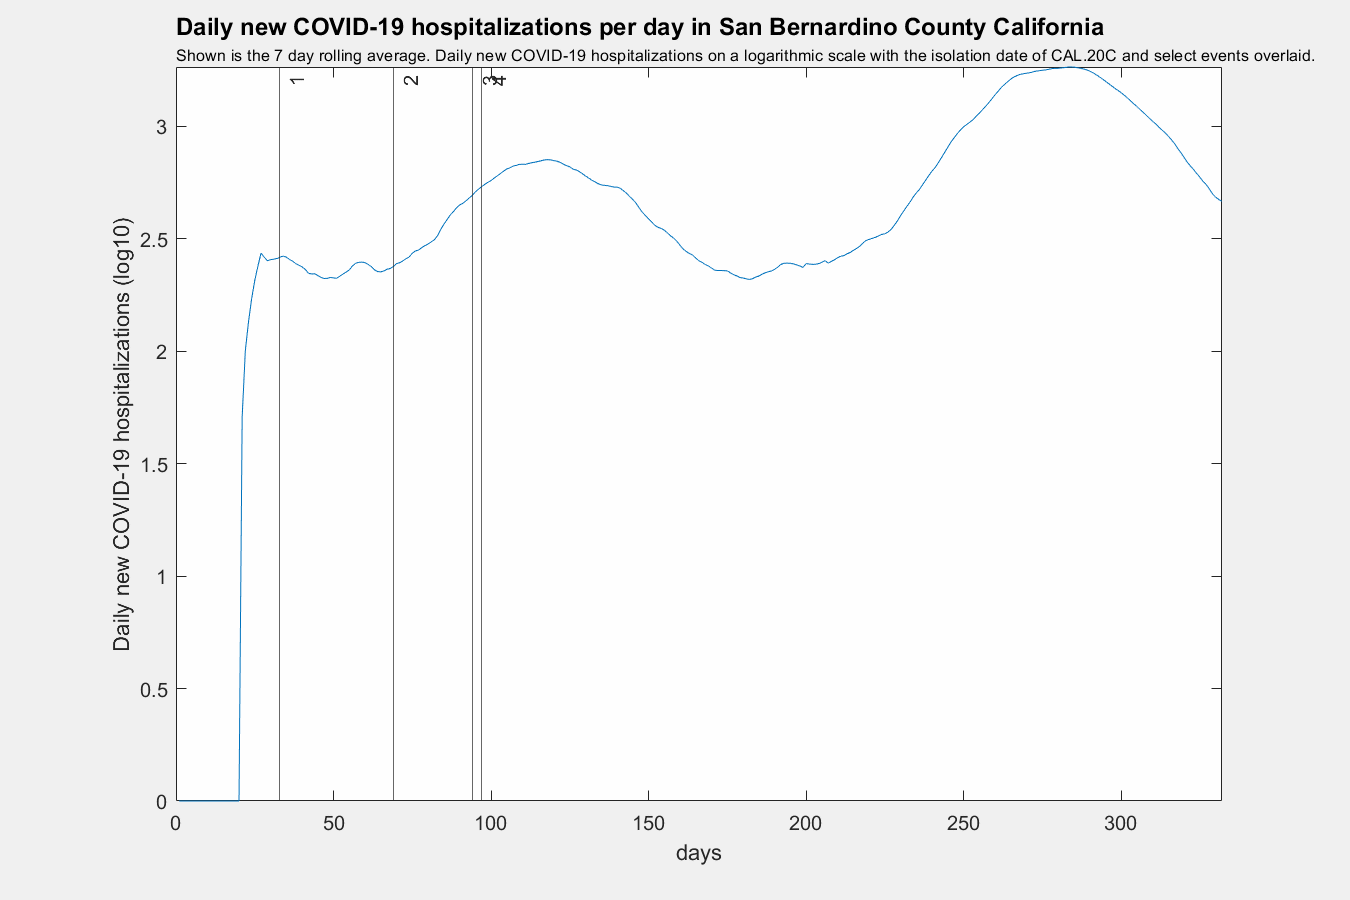
\includegraphics[width=0.26\textwidth]{images/san_bernardino_hospitalizations_CAL20C_log.png}}
	\subfigure[]{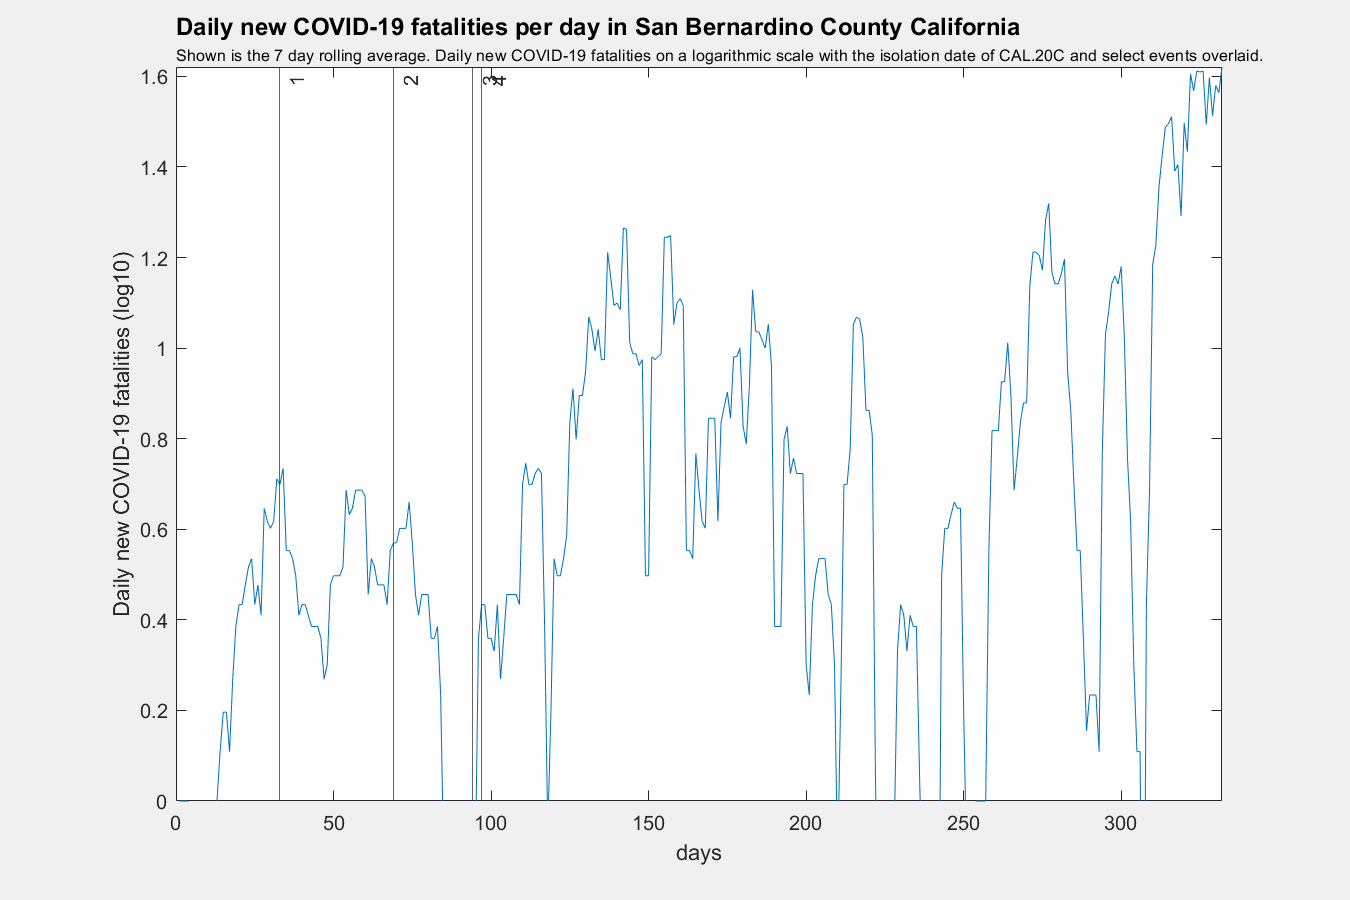
\includegraphics[width=0.26\textwidth]{images/san_bernardino_fatalities_CAL20C_log.png}}
	\subfigure[]{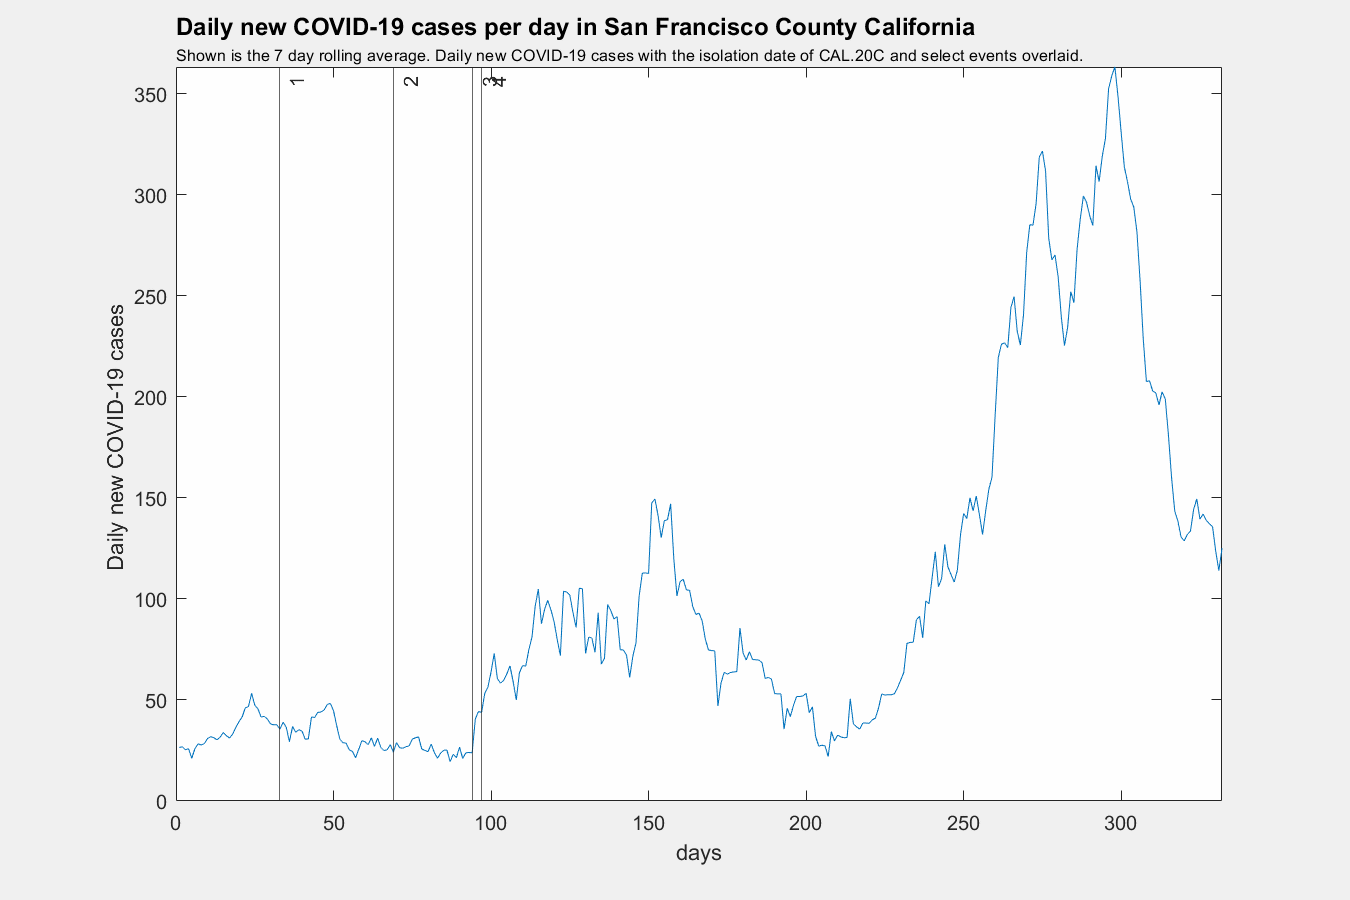
\includegraphics[width=0.26\textwidth]{images/san_francisco_cases_CAL20C.png}}
	\subfigure[]{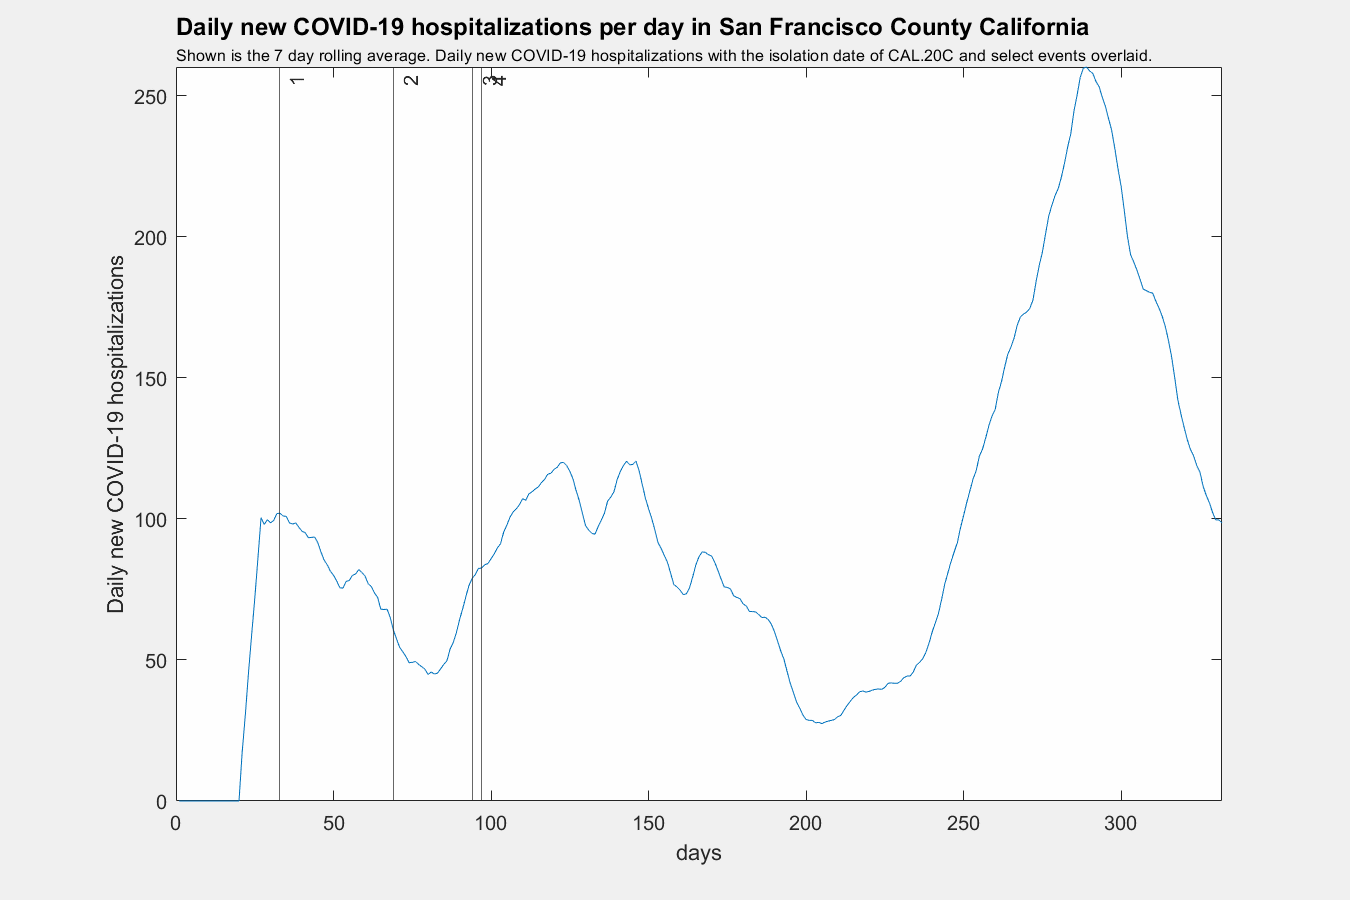
\includegraphics[width=0.26\textwidth]{images/san_francisco_hospitalizations_CAL20C.png}}
	\subfigure[]{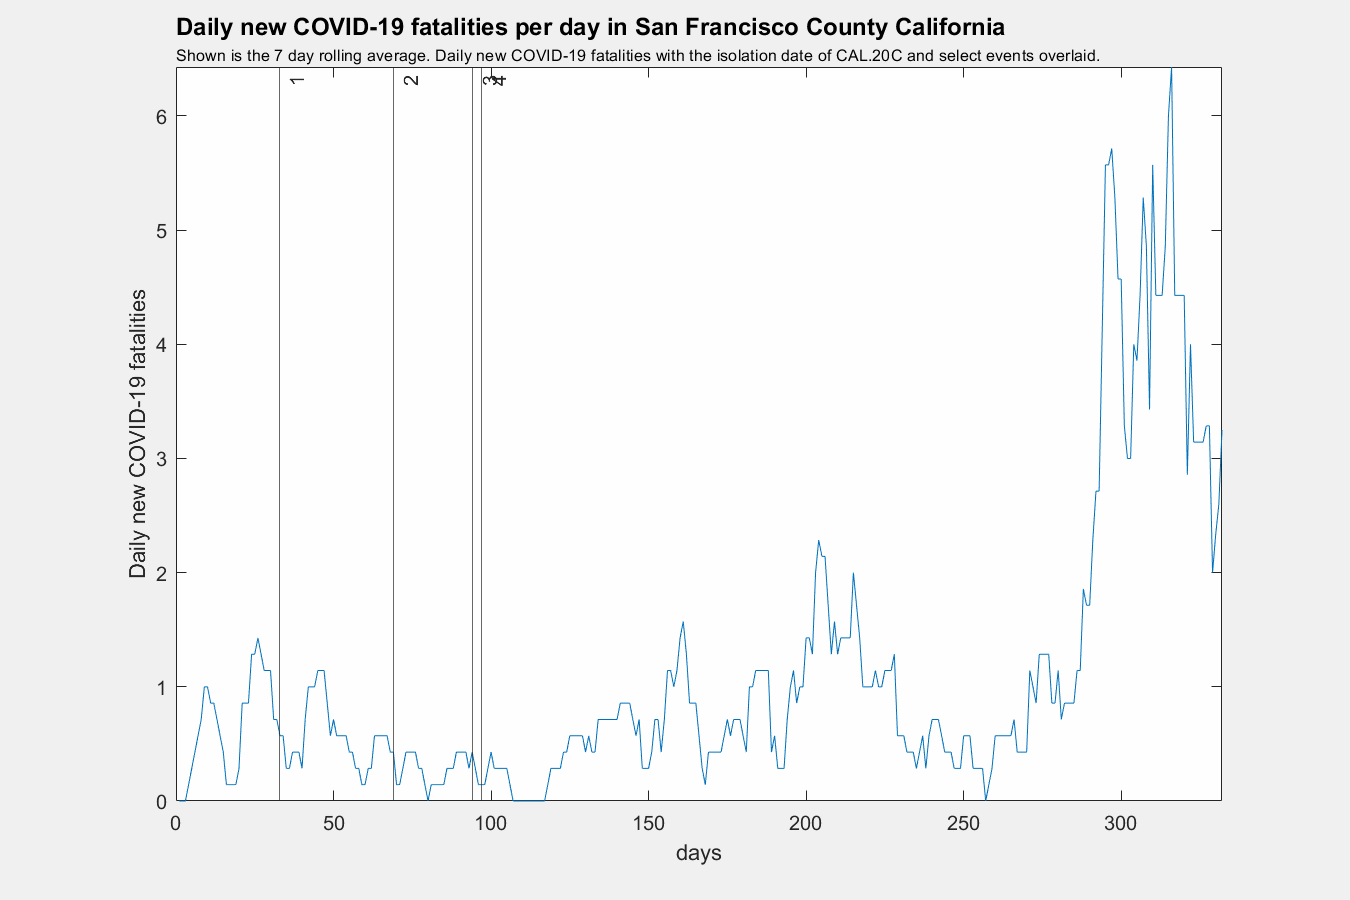
\includegraphics[width=0.26\textwidth]{images/san_francisco_fatalities_CAL20C.png}}
	\subfigure[]{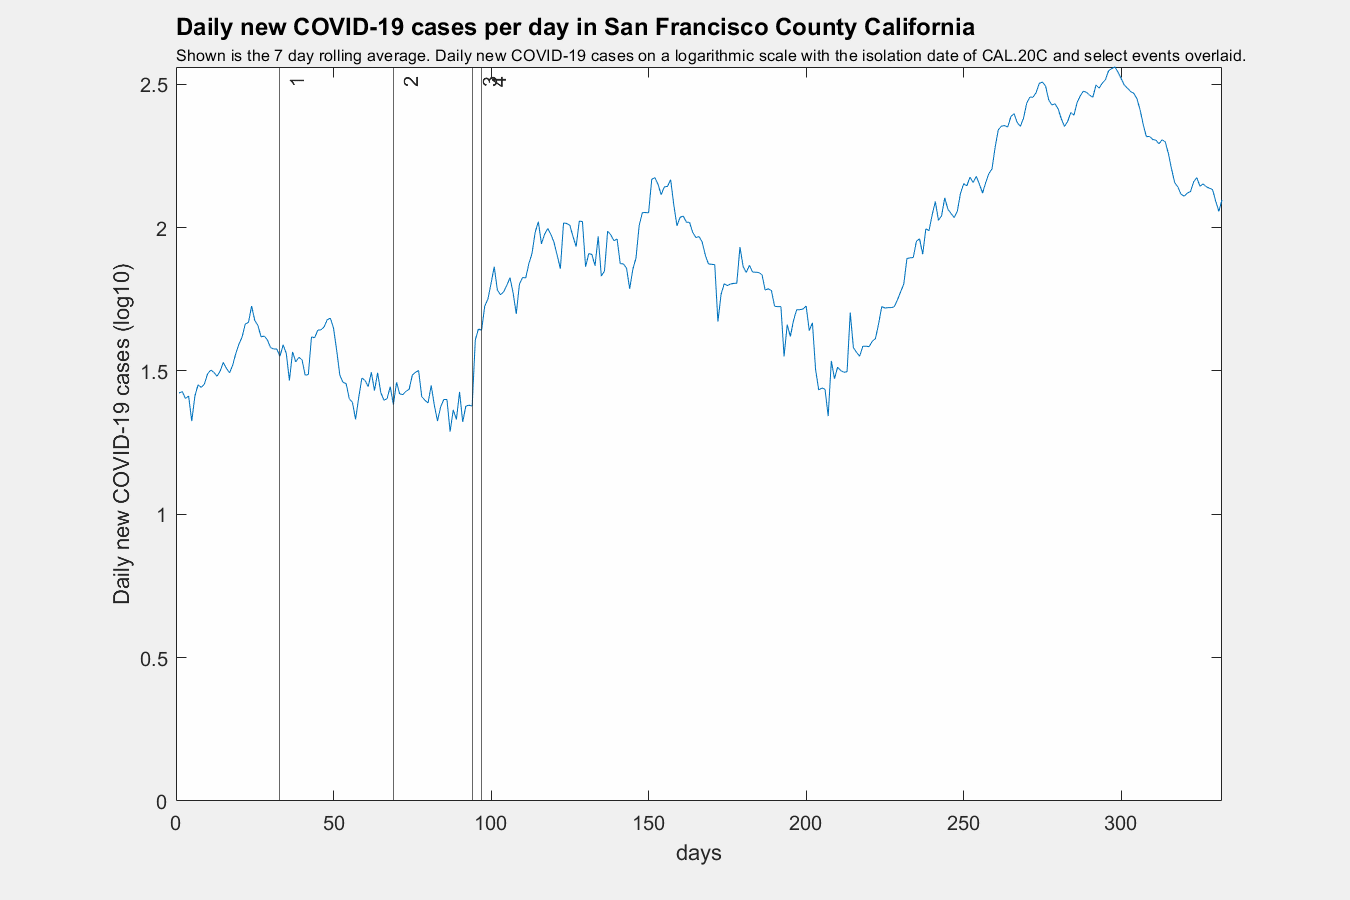
\includegraphics[width=0.26\textwidth]{images/san_francisco_cases_CAL20C_log.png}}
	\subfigure[]{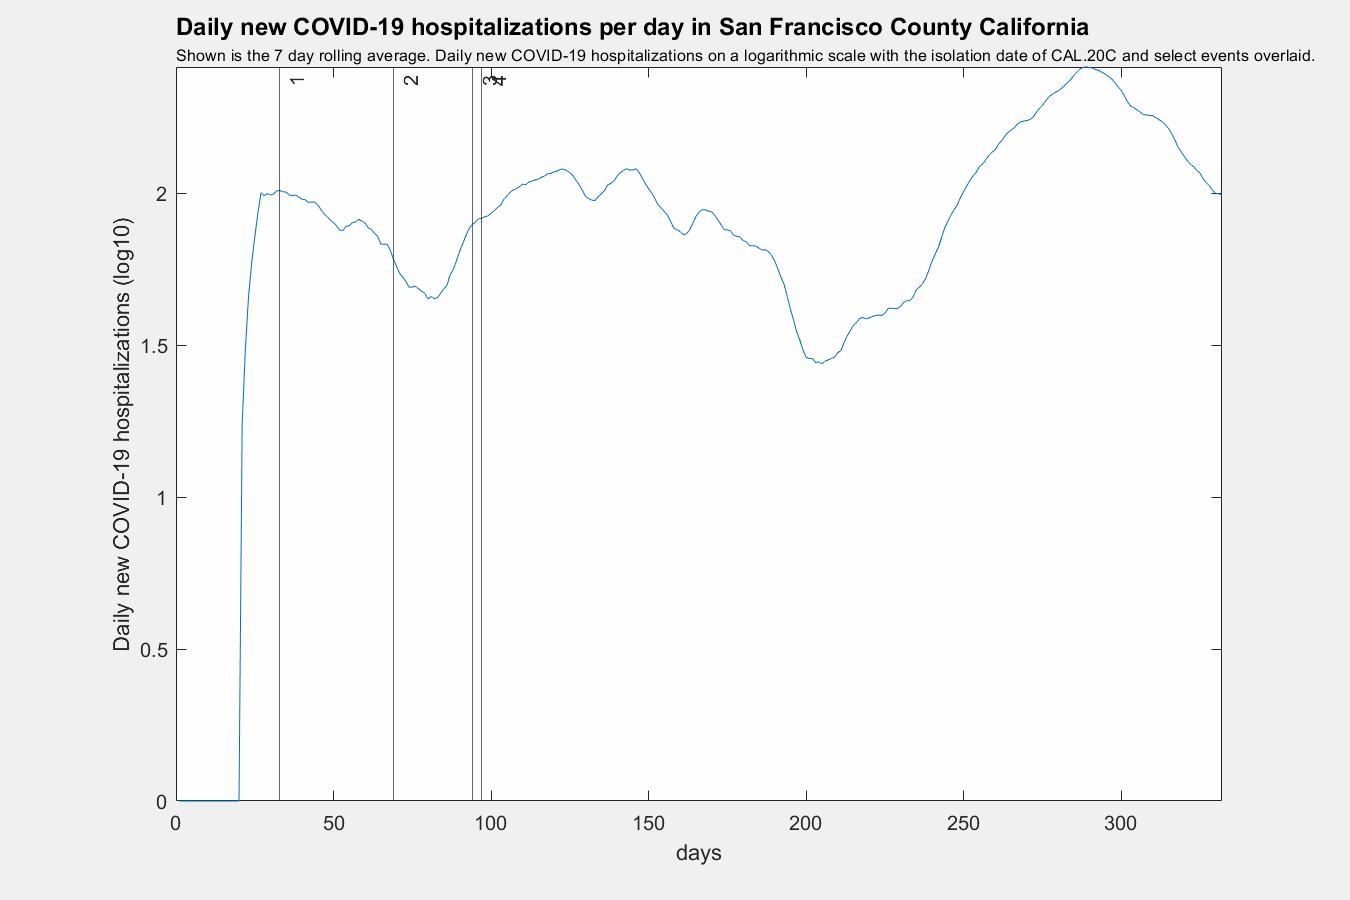
\includegraphics[width=0.26\textwidth]{images/san_francisco_hospitalizations_CAL20C_log.png}}
	\subfigure[]{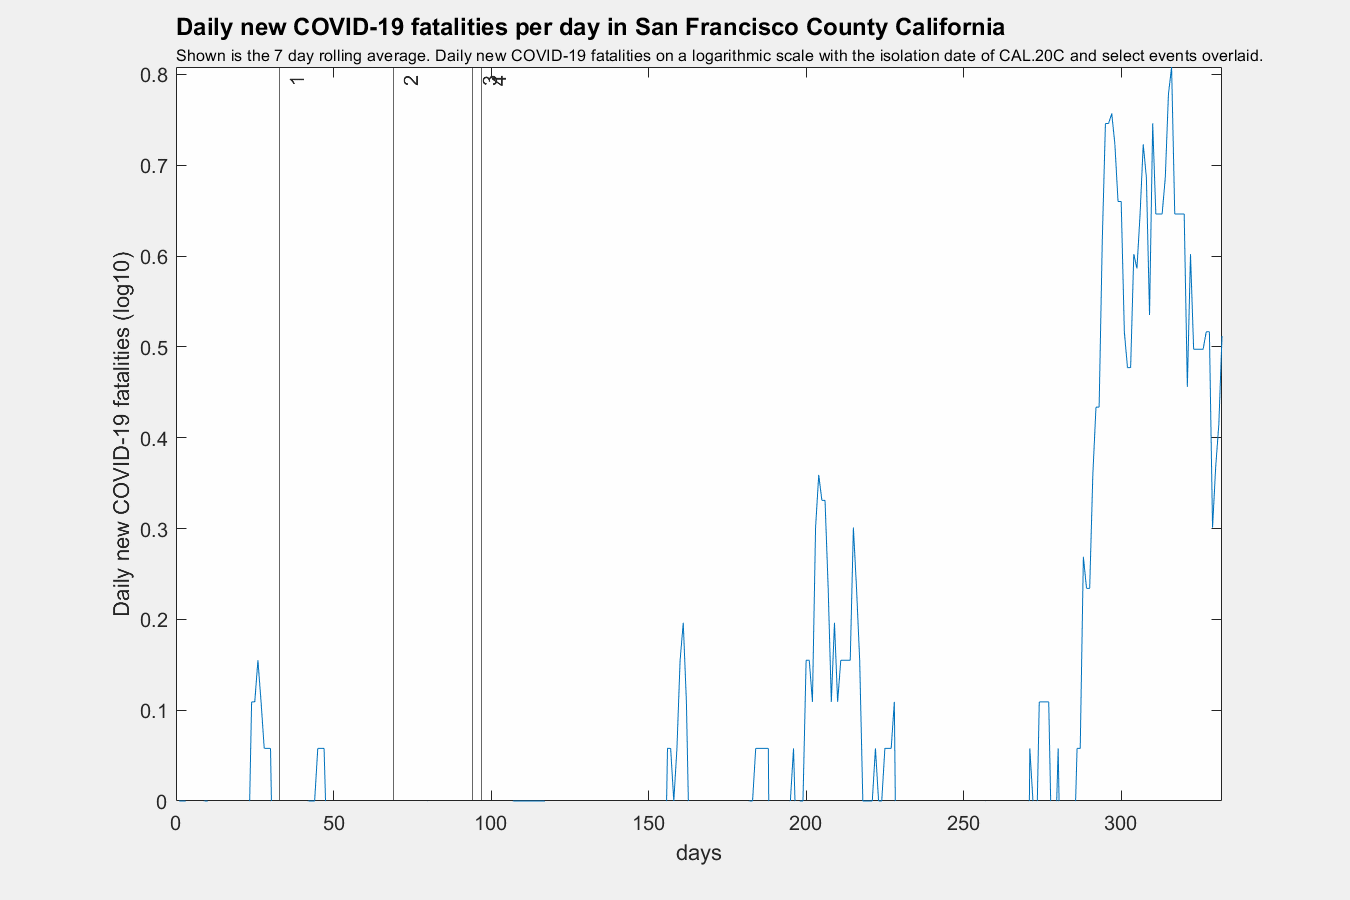
\includegraphics[width=0.26\textwidth]{images/san_francisco_fatalities_CAL20C_log.png}}
		\caption{(a-f) Los Angeles County; (g-l) San Bernardino County; (m-r) San Francisco County }
	\label{fig:foobar}
\end{figure}
\FloatBarrier
\vspace{5mm}

\subsection{Texas}

\begin{figure}[!h]
	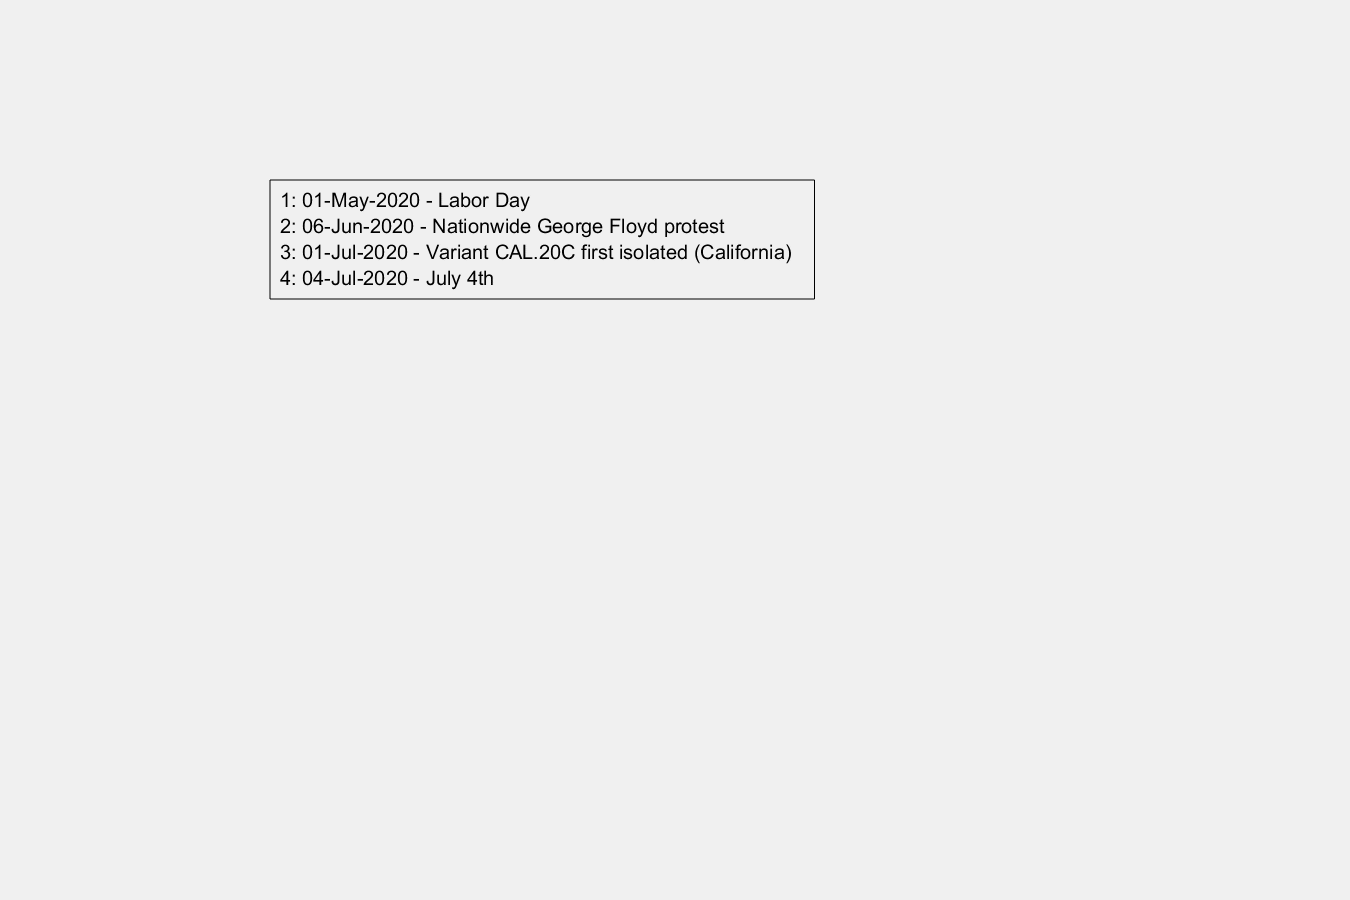
\includegraphics[width=\linewidth]{legends/CAL20C_legend.png}
	\caption{}
	\label{fig:legends/CAL20C_legendLabel}
\end{figure}

\begin{figure}
	\centering
	\subfigure[]{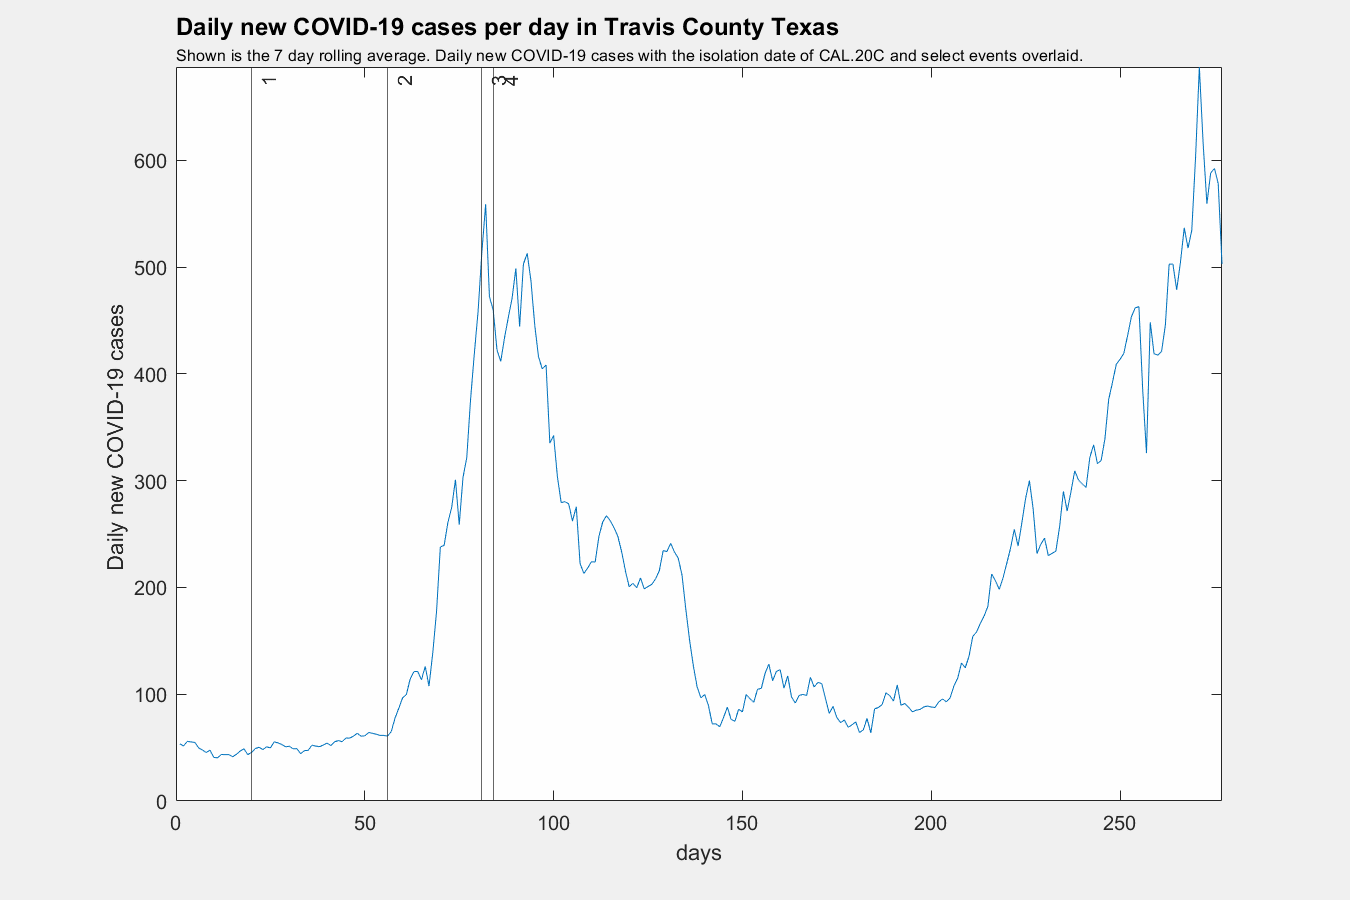
\includegraphics[width=0.26\textwidth]{images/travis_cases_CAL20C.png}}
	\subfigure[]{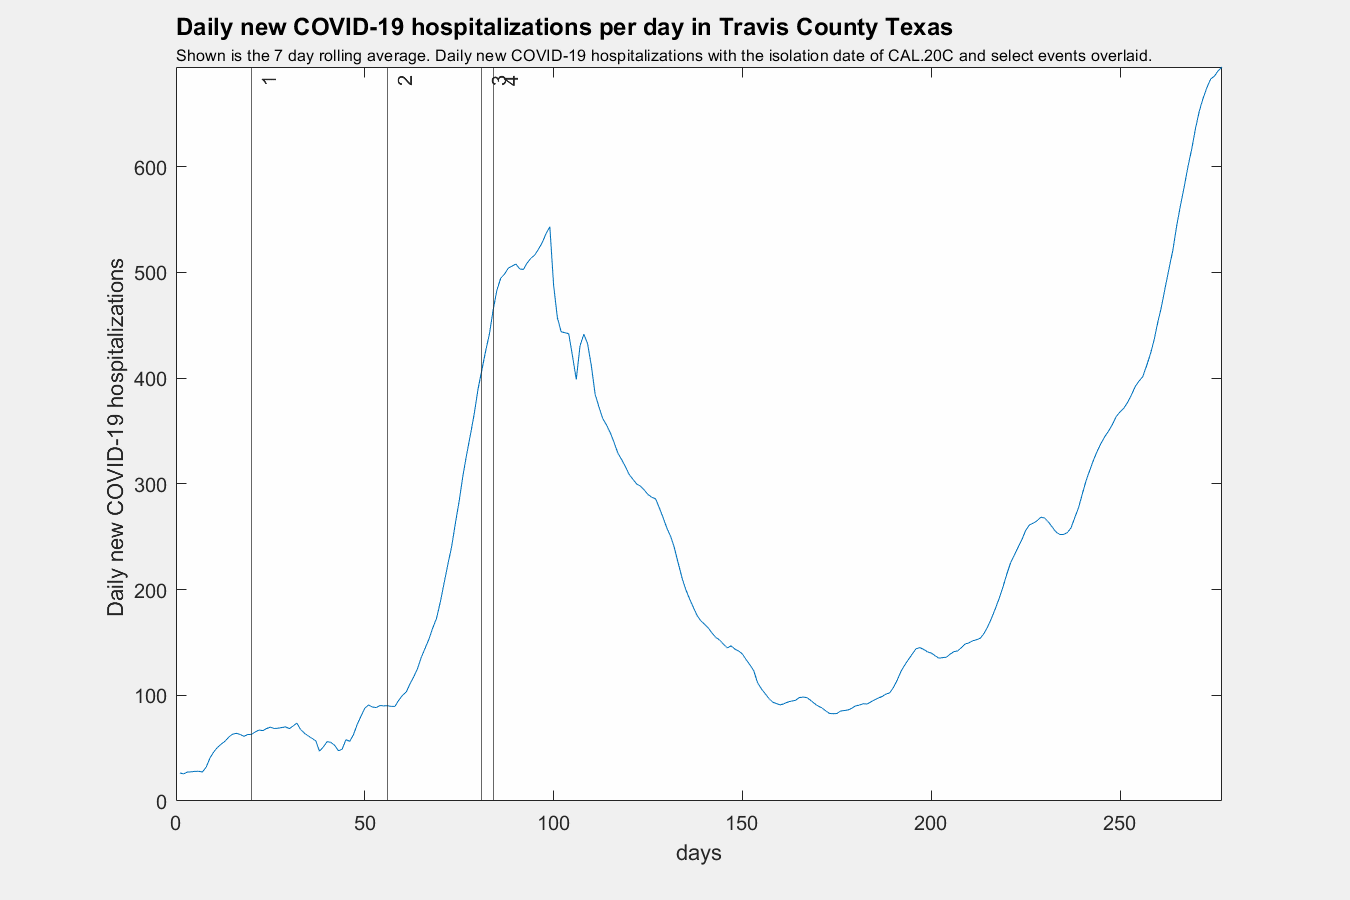
\includegraphics[width=0.26\textwidth]{images/travis_hospitalizations_CAL20C.png}}
	\subfigure[]{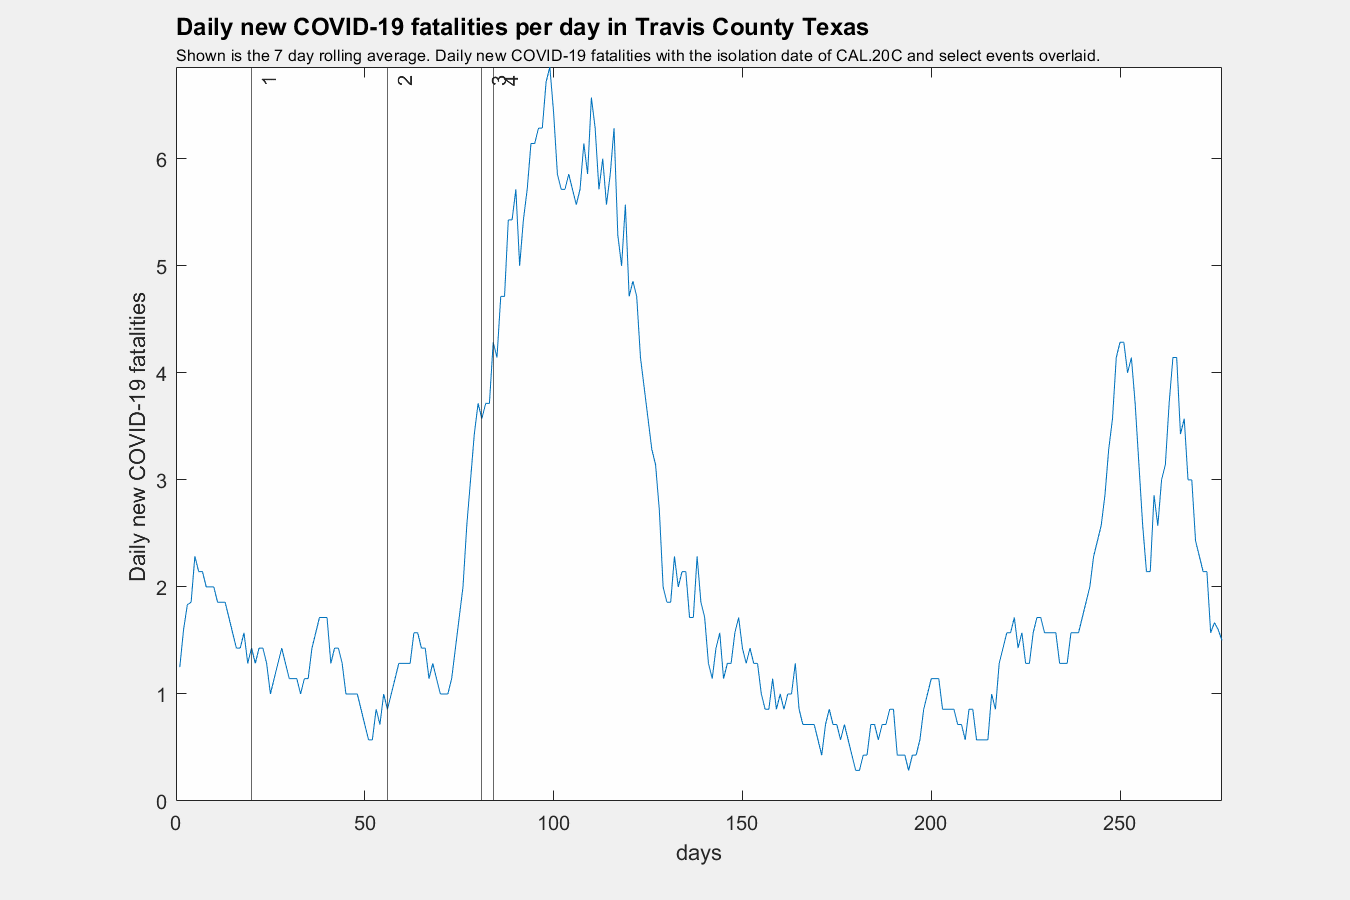
\includegraphics[width=0.26\textwidth]{images/travis_fatalities_CAL20C.png}}
	\subfigure[]{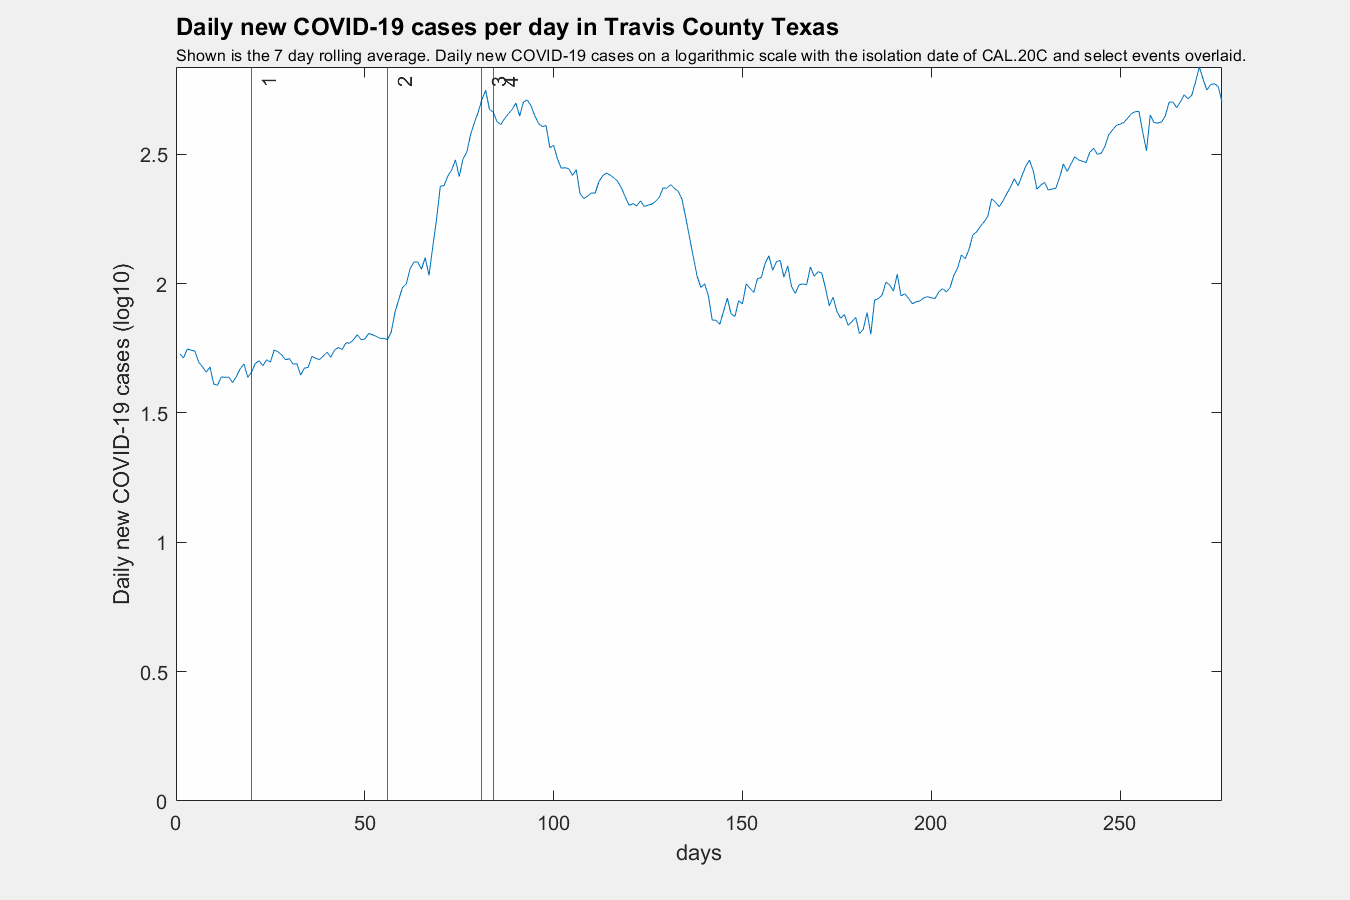
\includegraphics[width=0.26\textwidth]{images/travis_cases_CAL20C_log.png}}
	\subfigure[]{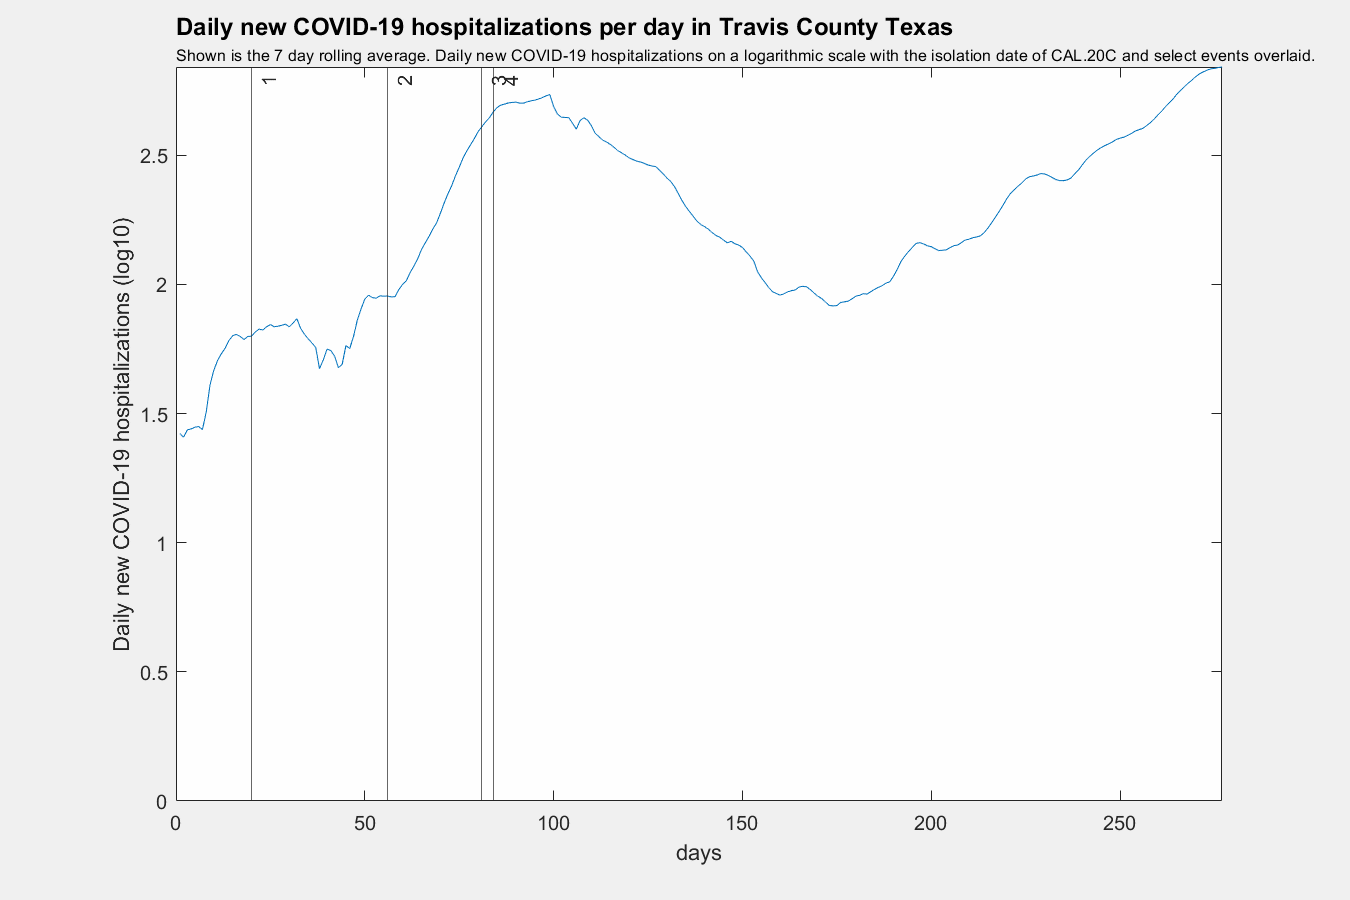
\includegraphics[width=0.26\textwidth]{images/travis_hospitalizations_CAL20C_log.png}}
	\subfigure[]{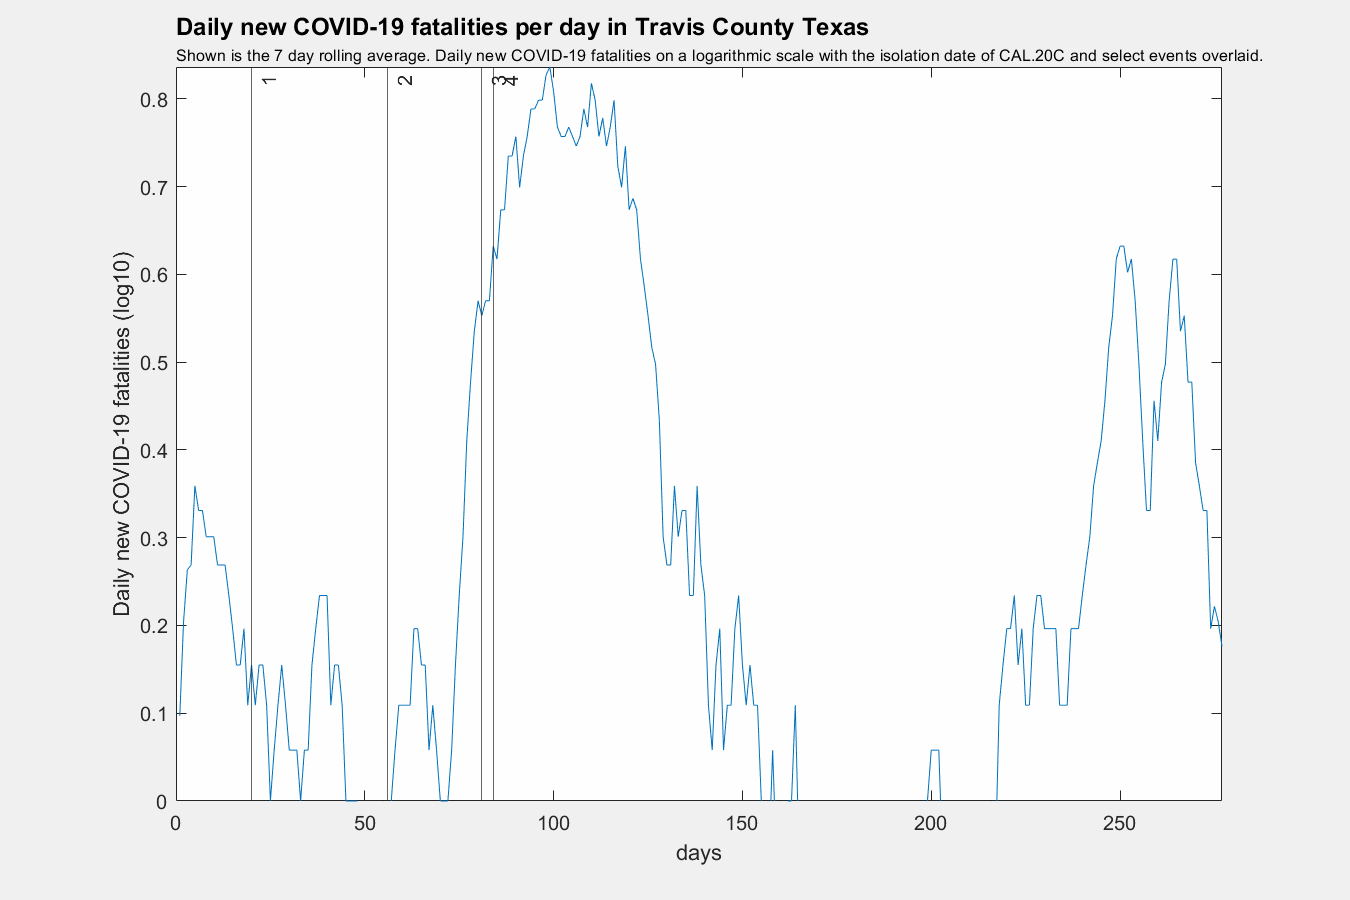
\includegraphics[width=0.26\textwidth]{images/travis_fatalities_CAL20C_log.png}}
	\subfigure[]{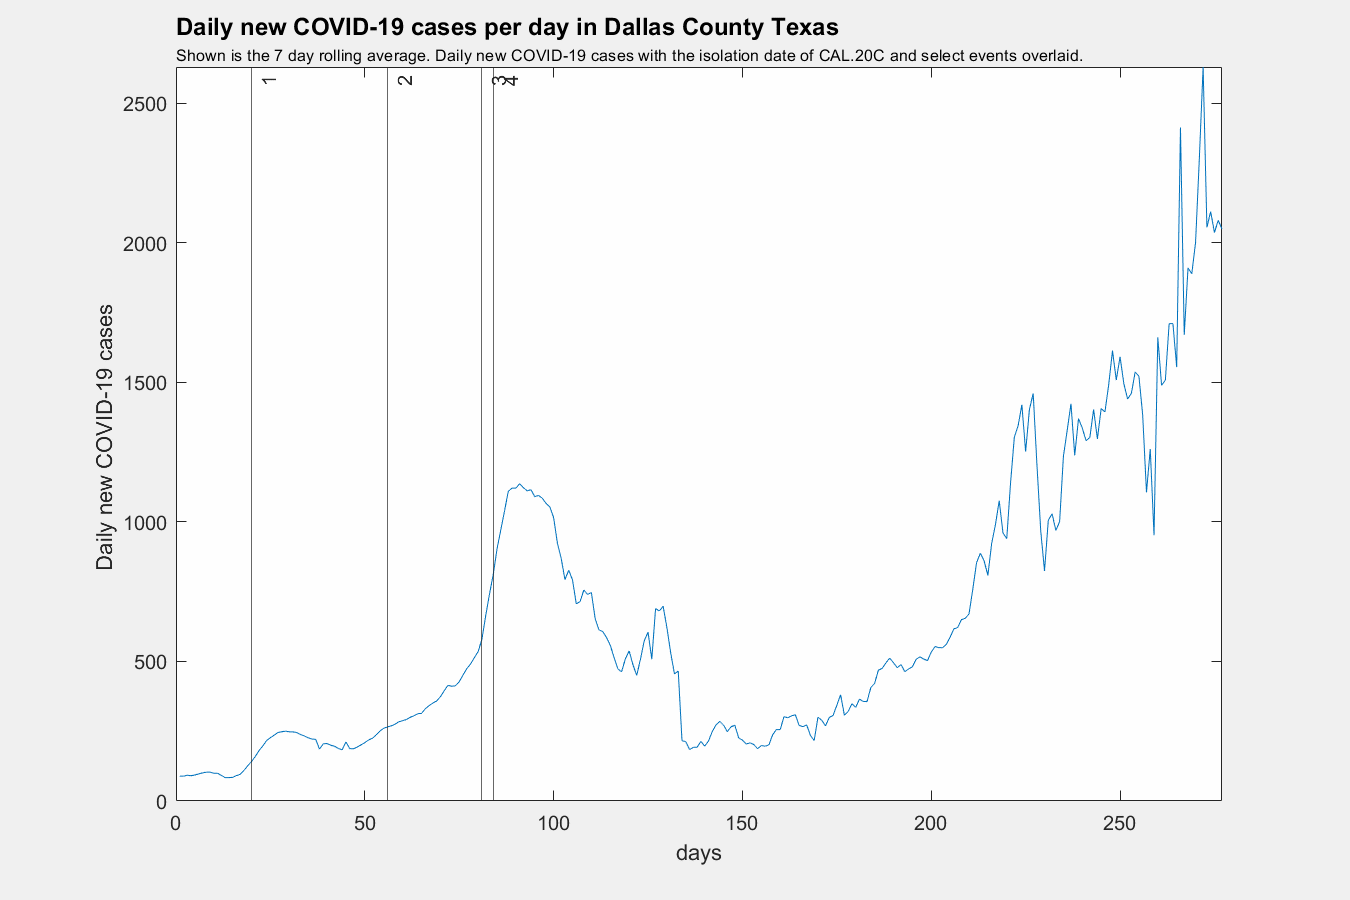
\includegraphics[width=0.26\textwidth]{images/dallas_cases_CAL20C.png}}
	\subfigure[]{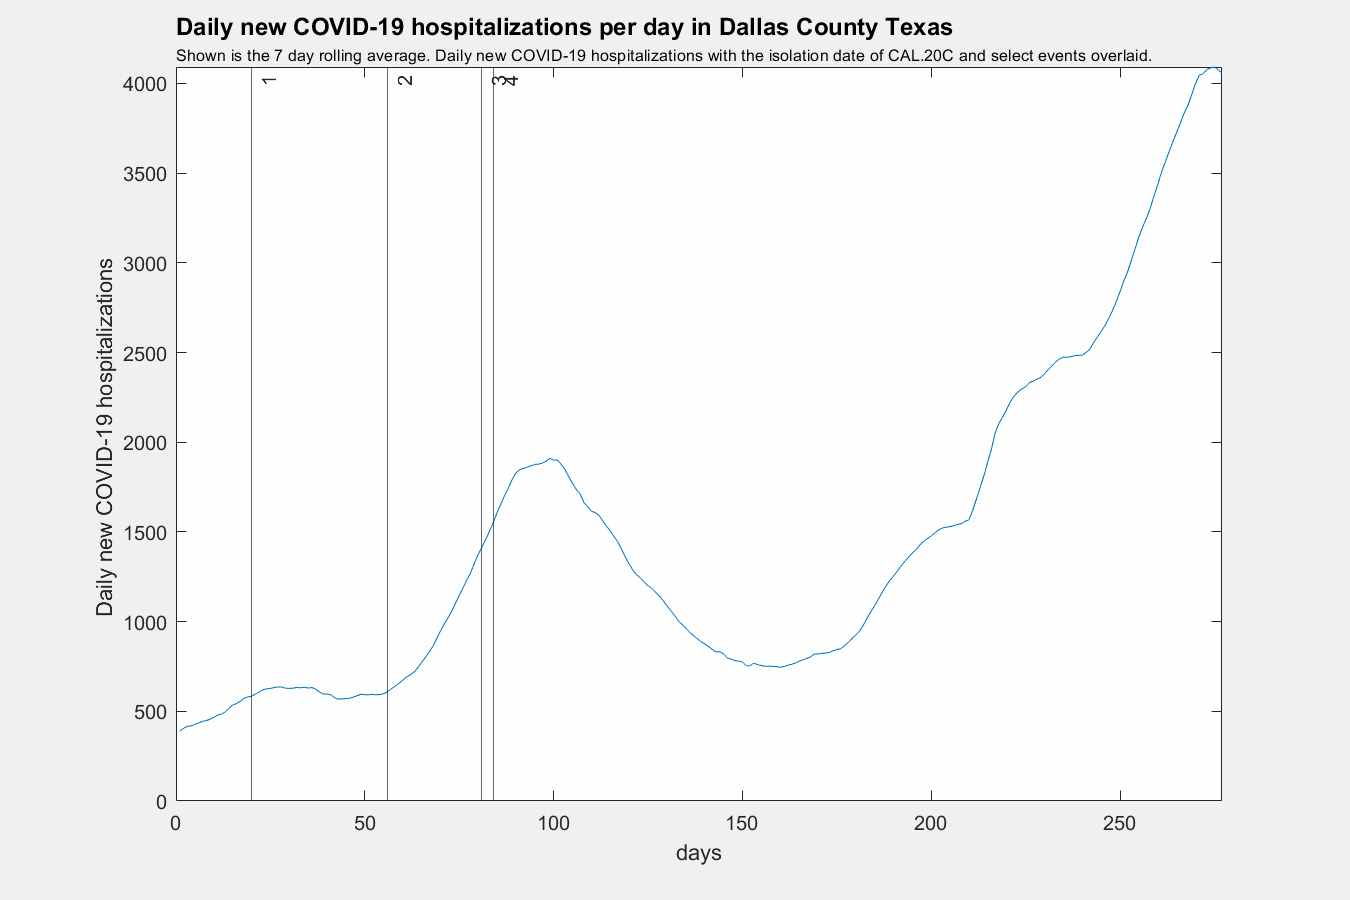
\includegraphics[width=0.26\textwidth]{images/dallas_hospitalizations_CAL20C.png}}
	\subfigure[]{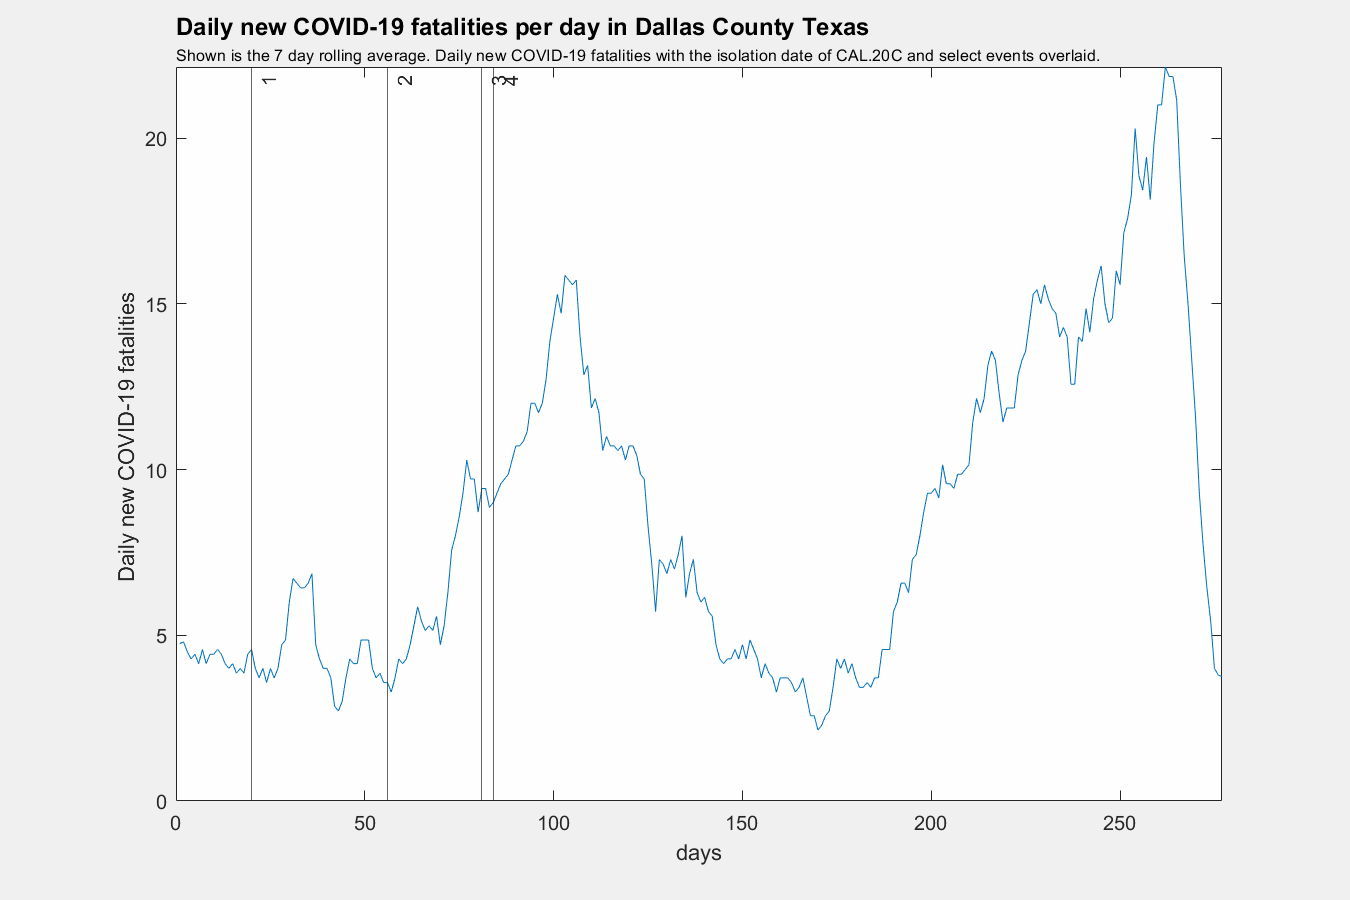
\includegraphics[width=0.26\textwidth]{images/dallas_fatalities_CAL20C.png}}
	\subfigure[]{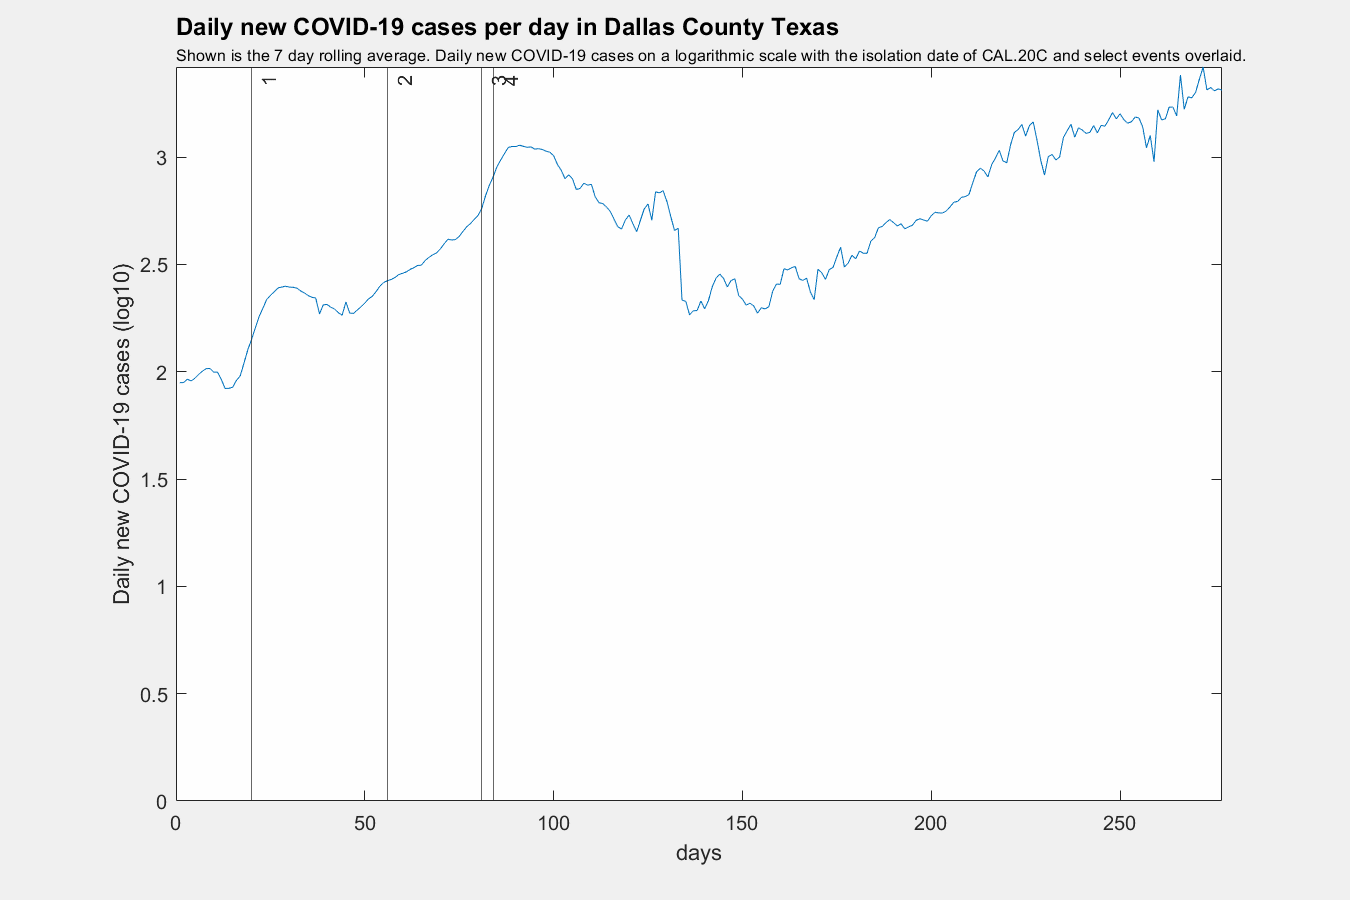
\includegraphics[width=0.26\textwidth]{images/dallas_cases_CAL20C_log.png}}
	\subfigure[]{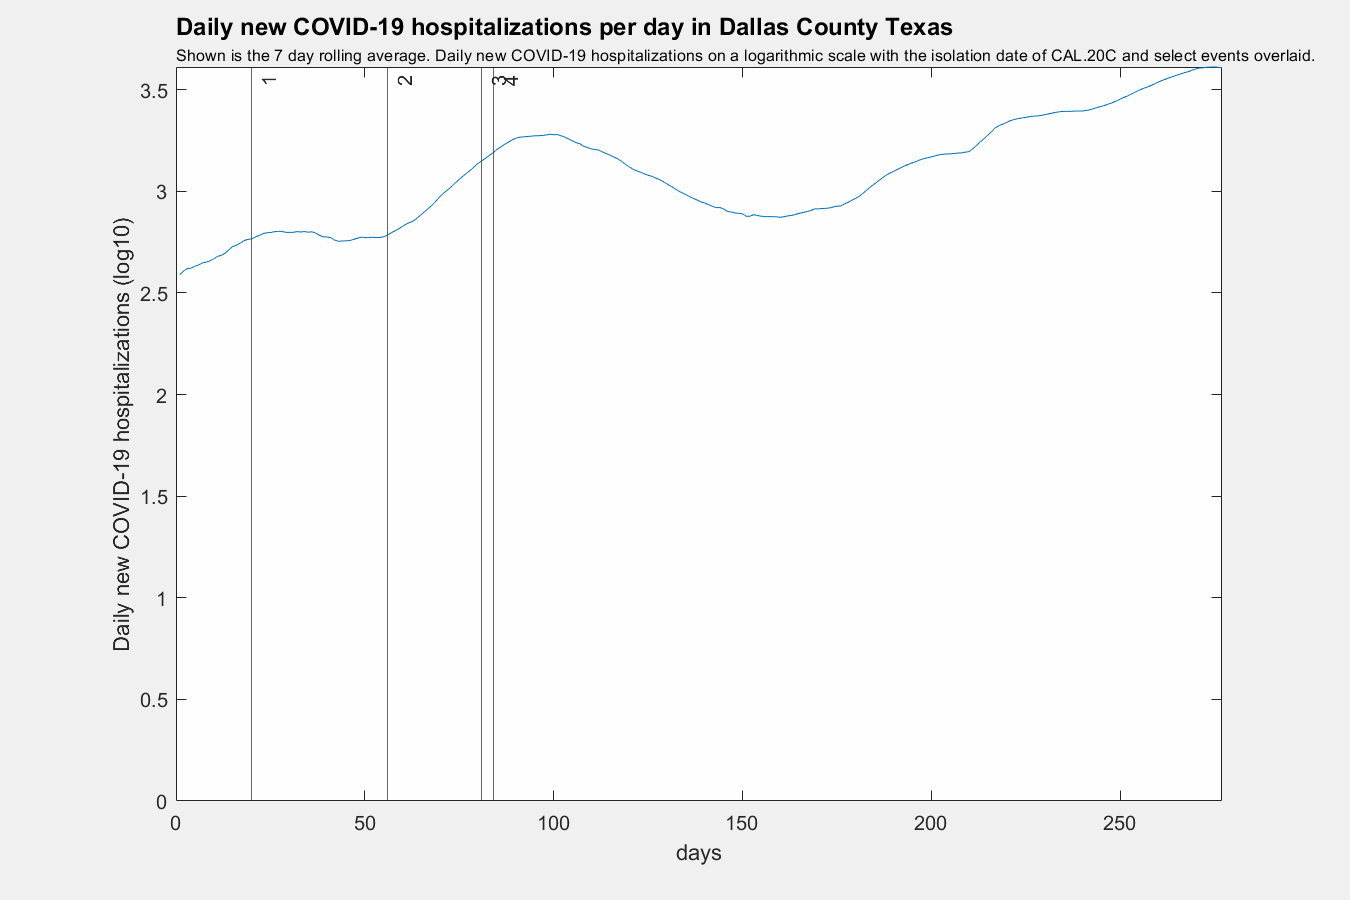
\includegraphics[width=0.26\textwidth]{images/dallas_hospitalizations_CAL20C_log.png}}
	\subfigure[]{\includegraphics[width=0.26\textwidth]{images/dallas_fatalities_CAL20C_log.png}}
	\subfigure[]{\includegraphics[width=0.26\textwidth]{images/harris_cases_CAL20C.png}}
	\subfigure[]{\includegraphics[width=0.26\textwidth]{images/harris_hospitalizations_CAL20C.png}}
	\subfigure[]{\includegraphics[width=0.26\textwidth]{images/harris_fatalities_CAL20C.png}}
	\subfigure[]{\includegraphics[width=0.26\textwidth]{images/harris_cases_CAL20C_log.png}}
	\subfigure[]{\includegraphics[width=0.26\textwidth]{images/harris_hospitalizations_CAL20C_log.png}}
	\subfigure[]{\includegraphics[width=0.26\textwidth]{images/harris_fatalities_CAL20C_log.png}}
	\caption{(a-f) Travis County; (g-l) Dallas County; (m-r) Harris County}
	\label{fig:foobar}
\end{figure}
\FloatBarrier
\vspace{5mm}



\section{B.1.1.7 and Nearby Significant Events}

\subsection{Florida}

\begin{figure}[!h]
	\includegraphics[width=\linewidth]{legends/B117_legend.png}
	\caption{}
	\label{fig:legends/B117_legendLabel}
\end{figure}

\begin{figure}
	\centering
	\subfigure[]{\includegraphics[width=0.26\textwidth]{images/dade_cases_B117.png}}
	\subfigure[]{\includegraphics[width=0.26\textwidth]{images/dade_hospitalizations_B117.png}}
	\subfigure[]{\includegraphics[width=0.26\textwidth]{images/dade_fatalities_B117.png}}
	\subfigure[]{\includegraphics[width=0.26\textwidth]{images/dade_cases_B117_log.png}}
	\subfigure[]{\includegraphics[width=0.26\textwidth]{images/dade_hospitalizations_B117_log.png}}
	\subfigure[]{\includegraphics[width=0.26\textwidth]{images/dade_fatalities_B117_log.png}}
	\subfigure[]{\includegraphics[width=0.26\textwidth]{images/broward_cases_B117.png}}
	\subfigure[]{\includegraphics[width=0.26\textwidth]{images/broward_hospitalizations_B117.png}}
	\subfigure[]{\includegraphics[width=0.26\textwidth]{images/broward_fatalities_B117.png}}
	\subfigure[]{\includegraphics[width=0.26\textwidth]{images/broward_cases_B117_log.png}}
	\subfigure[]{\includegraphics[width=0.26\textwidth]{images/broward_hospitalizations_B117_log.png}}
	\subfigure[]{\includegraphics[width=0.26\textwidth]{images/broward_fatalities_B117_log.png}}
	\subfigure[]{\includegraphics[width=0.26\textwidth]{images/orange_cases_B117.png}}
	\subfigure[]{\includegraphics[width=0.26\textwidth]{images/orange_hospitalizations_B117.png}}
	\subfigure[]{\includegraphics[width=0.26\textwidth]{images/orange_fatalities_B117.png}}
	\subfigure[]{\includegraphics[width=0.26\textwidth]{images/orange_cases_B117_log.png}}
	\subfigure[]{\includegraphics[width=0.26\textwidth]{images/orange_hospitalizations_B117_log.png}}
	\subfigure[]{\includegraphics[width=0.26\textwidth]{images/orange_fatalities_B117_log.png}}
		\caption{(a-f) Dade County; (g-l) Broward County; (m-r) Orange County}
	\label{fig:foobar}
\end{figure}
\FloatBarrier
\vspace{5mm}

\subsection{California}

\begin{figure}[!h]
	\includegraphics[width=\linewidth]{legends/B117_legend.png}
	\caption{}
	\label{fig:legends/B117_legendLabel}
\end{figure}

\begin{figure}
	\centering
	\subfigure[]{\includegraphics[width=0.26\textwidth]{images/los_angeles_cases_B117.png}}
	\subfigure[]{\includegraphics[width=0.26\textwidth]{images/los_angeles_hospitalizations_B117.png}}
	\subfigure[]{\includegraphics[width=0.26\textwidth]{images/los_angeles_fatalities_B117.png}}
	\subfigure[]{\includegraphics[width=0.26\textwidth]{images/los_angeles_cases_B117_log.png}}
	\subfigure[]{\includegraphics[width=0.26\textwidth]{images/los_angeles_hospitalizations_B117_log.png}}
	\subfigure[]{\includegraphics[width=0.26\textwidth]{images/los_angeles_fatalities_B117_log.png}}
	\subfigure[]{\includegraphics[width=0.26\textwidth]{images/san_bernardino_cases_B117.png}}
	\subfigure[]{\includegraphics[width=0.26\textwidth]{images/san_bernardino_hospitalizations_B117.png}}
	\subfigure[]{\includegraphics[width=0.26\textwidth]{images/san_bernardino_fatalities_B117.png}}
	\subfigure[]{\includegraphics[width=0.26\textwidth]{images/san_bernardino_cases_B117_log.png}}
	\subfigure[]{\includegraphics[width=0.26\textwidth]{images/san_bernardino_hospitalizations_B117_log.png}}
	\subfigure[]{\includegraphics[width=0.26\textwidth]{images/san_bernardino_fatalities_B117_log.png}}
	\subfigure[]{\includegraphics[width=0.26\textwidth]{images/san_francisco_cases_B117.png}}
	\subfigure[]{\includegraphics[width=0.26\textwidth]{images/san_francisco_hospitalizations_B117.png}}
	\subfigure[]{\includegraphics[width=0.26\textwidth]{images/san_francisco_fatalities_B117.png}}
	\subfigure[]{\includegraphics[width=0.26\textwidth]{images/san_francisco_cases_B117_log.png}}
	\subfigure[]{\includegraphics[width=0.26\textwidth]{images/san_francisco_hospitalizations_B117_log.png}}
	\subfigure[]{\includegraphics[width=0.26\textwidth]{images/san_francisco_fatalities_B117_log.png}}
		\caption{(a-f) Los Angeles County; (g-l) San Bernardino County; (m-r) San Francisco County}
	\label{fig:foobar}
\end{figure}
\FloatBarrier
\vspace{5mm}

\subsection{Texas}

\begin{figure}[!h]
	\includegraphics[width=\linewidth]{legends/B117_legend.png}
	\caption{}
	\label{fig:legends/B117_legendLabel}
\end{figure}
\begin{figure}
	\centering
	\subfigure[]{\includegraphics[width=0.26\textwidth]{images/travis_cases_B117.png}}
	\subfigure[]{\includegraphics[width=0.26\textwidth]{images/travis_hospitalizations_B117.png}}
	\subfigure[]{\includegraphics[width=0.26\textwidth]{images/travis_fatalities_B117.png}}
	\subfigure[]{\includegraphics[width=0.26\textwidth]{images/travis_cases_B117_log.png}}
	\subfigure[]{\includegraphics[width=0.26\textwidth]{images/travis_hospitalizations_B117_log.png}}
	\subfigure[]{\includegraphics[width=0.26\textwidth]{images/travis_fatalities_B117_log.png}}
	\subfigure[]{\includegraphics[width=0.26\textwidth]{images/dallas_cases_B117.png}}
	\subfigure[]{\includegraphics[width=0.26\textwidth]{images/dallas_hospitalizations_B117.png}}
	\subfigure[]{\includegraphics[width=0.26\textwidth]{images/dallas_fatalities_B117.png}}
	\subfigure[]{\includegraphics[width=0.26\textwidth]{images/dallas_cases_B117_log.png}}
	\subfigure[]{\includegraphics[width=0.26\textwidth]{images/dallas_hospitalizations_B117_log.png}}
	\subfigure[]{\includegraphics[width=0.26\textwidth]{images/dallas_fatalities_B117_log.png}}
	\subfigure[]{\includegraphics[width=0.26\textwidth]{images/harris_cases_B117.png}}
	\subfigure[]{\includegraphics[width=0.26\textwidth]{images/harris_hospitalizations_B117.png}}
	\subfigure[]{\includegraphics[width=0.26\textwidth]{images/harris_fatalities_B117.png}}
	\subfigure[]{\includegraphics[width=0.26\textwidth]{images/harris_cases_B117_log.png}}
	\subfigure[]{\includegraphics[width=0.26\textwidth]{images/harris_hospitalizations_B117_log.png}}
	\subfigure[]{\includegraphics[width=0.26\textwidth]{images/harris_fatalities_B117_log.png}}
	\caption{(a-f) Travis County; (g-l) Dallas County; (m-r) Harris County}
\label{fig:foobar}
\end{figure}
\FloatBarrier
\vspace{5mm}

\section{COVID-19 Vaccine Rollout and Administration}


\subsection{Florida}

\begin{figure}[!h]
	\includegraphics[width=\linewidth]{legends/vaccine_rollout_legend.png}
	\caption{}
	\label{fig:legends/vaccine_rollout_legendLabel}
\end{figure}

\begin{figure}
	\centering
	\subfigure[]{\includegraphics[width=0.32\textwidth]{images/dade_cases_vaccine_rollout_log.png}}
	\subfigure[]{\includegraphics[width=0.32\textwidth]{images/broward_cases_vaccine_rollout_log.png}}
	\subfigure[]{\includegraphics[width=0.32\textwidth]{images/orange_cases_vaccine_rollout_log.png}}
	\subfigure[]{\includegraphics[width=0.32\textwidth]{images/los_angeles_cases_vaccine_rollout_log.png}}
	\subfigure[]{\includegraphics[width=0.32\textwidth]{images/san_bernardino_cases_vaccine_rollout_log.png}}
	\subfigure[]{\includegraphics[width=0.32\textwidth]{images/san_francisco_cases_vaccine_rollout_log.png}}
	\subfigure[]{\includegraphics[width=0.32\textwidth]{images/travis_cases_vaccine_rollout_log.png}}
	\subfigure[]{\includegraphics[width=0.32\textwidth]{images/dallas_cases_vaccine_rollout_log.png}}
	\subfigure[]{\includegraphics[width=0.32\textwidth]{images/harris_cases_vaccine_rollout_log.png}}
	\caption{(a) Dade County, Florida (b) Broward County, Florida (c) Orange County, Florida (d) Los Angeles County, California (e) San Bernardino County California (f) San Francisco County California (g) Travis County, Texas (h) Dallas County, Texas (i) Harris County, Texas}
	\label{fig:foobar}
\end{figure}
\FloatBarrier
\vspace{5mm}

\subsection{Vaccine Rollout, Administration and Hospitalizations}

\begin{figure}[!h]
	\includegraphics[width=\linewidth]{legends/vaccine_rollout_legend.png}
	\caption{}
	\label{fig:legends/vaccine_rollout_legendLabel}
\end{figure}

\begin{figure}
	\centering
	\subfigure[]{\includegraphics[width=0.32\textwidth]{images/dade_hospitalizations_vaccine_rollout_log.png}}
	\subfigure[]{\includegraphics[width=0.32\textwidth]{images/broward_hospitalizations_vaccine_rollout_log.png}}
	\subfigure[]{\includegraphics[width=0.32\textwidth]{images/orange_hospitalizations_vaccine_rollout_log.png}}
	\subfigure[]{\includegraphics[width=0.32\textwidth]{images/los_angeles_hospitalizations_vaccine_rollout_log.png}}
	\subfigure[]{\includegraphics[width=0.32\textwidth]{images/san_bernardino_hospitalizations_vaccine_rollout_log.png}}
	\subfigure[]{\includegraphics[width=0.32\textwidth]{images/san_francisco_hospitalizations_vaccine_rollout_log.png}}
	\subfigure[]{\includegraphics[width=0.32\textwidth]{images/travis_hospitalizations_vaccine_rollout_log.png}}
	\subfigure[]{\includegraphics[width=0.32\textwidth]{images/dallas_hospitalizations_vaccine_rollout_log.png}}
	\subfigure[]{\includegraphics[width=0.32\textwidth]{images/harris_hospitalizations_vaccine_rollout_log.png}}
	\caption{(a) Dade County, Florida (b) Broward County, Florida (c) Orange County, Florida (d) Los Angeles County, California (e) San Bernardino County California (f) San Francisco County California (g) Travis County, Texas (h) Dallas County, Texas (i) Harris County, Texas}
	\label{fig:foobar}
\end{figure}
\FloatBarrier
\vspace{5mm}

\subsection{Vaccine Rollout, Administration and Fatalities}

\begin{figure}[!h]
	\includegraphics[width=\linewidth]{legends/vaccine_rollout_legend.png}
	\caption{}
	\label{fig:legends/vaccine_rollout_legendLabel}
\end{figure}

\begin{figure}
	\centering
	\subfigure[]{\includegraphics[width=0.32\textwidth]{images/dade_fatalities_vaccine_rollout_log.png}}
	\subfigure[]{\includegraphics[width=0.32\textwidth]{images/broward_fatalities_vaccine_rollout_log.png}}
	\subfigure[]{\includegraphics[width=0.32\textwidth]{images/orange_fatalities_vaccine_rollout_log.png}}
	\subfigure[]{\includegraphics[width=0.32\textwidth]{images/los_angeles_fatalities_vaccine_rollout_log.png}}
	\subfigure[]{\includegraphics[width=0.32\textwidth]{images/san_bernardino_fatalities_vaccine_rollout_log.png}}
	\subfigure[]{\includegraphics[width=0.32\textwidth]{images/san_francisco_fatalities_vaccine_rollout_log.png}}
	\subfigure[]{\includegraphics[width=0.32\textwidth]{images/travis_fatalities_vaccine_rollout_log.png}}
	\subfigure[]{\includegraphics[width=0.32\textwidth]{images/dallas_fatalities_vaccine_rollout_log.png}}
	\subfigure[]{\includegraphics[width=0.32\textwidth]{images/harris_fatalities_vaccine_rollout_log.png}}
	\caption{(a) Dade County, Florida (b) Broward County, Florida (c) Orange County, Florida (d) Los Angeles County, California (e) San Bernardino County California (f) San Francisco County California (g) Travis County, Texas (h) Dallas County, Texas (i) Harris County, Texas}
	\label{fig:foobar}
\end{figure}
\FloatBarrier
\vspace{5mm}

\subsection{Discussion of vaccine rollout and administration}

\vspace{5mm}

\section{George Floyd, Black Lives Matter, National Unrest}


\subsection{Black Lives Matter Events and COVID-19 Cases}

\begin{figure}[!h]
	\includegraphics[width=\linewidth]{legends/BLM_legend.png}
	\caption{}
	\label{fig:legends/BLM_legendLabel}
\end{figure}

\begin{figure}
	\centering
	\subfigure[]{\includegraphics[width=0.32\textwidth]{images/dade_cases_BLM_log.png}}
	\subfigure[]{\includegraphics[width=0.32\textwidth]{images/broward_cases_BLM_log.png}}
	\subfigure[]{\includegraphics[width=0.32\textwidth]{images/orange_cases_BLM_log.png}}
	\subfigure[]{\includegraphics[width=0.32\textwidth]{images/los_angeles_cases_BLM_log.png}}
	\subfigure[]{\includegraphics[width=0.32\textwidth]{images/san_bernardino_cases_BLM_log.png}}
	\subfigure[]{\includegraphics[width=0.32\textwidth]{images/san_francisco_cases_BLM_log.png}}
	\subfigure[]{\includegraphics[width=0.32\textwidth]{images/travis_cases_BLM_log.png}}
	\subfigure[]{\includegraphics[width=0.32\textwidth]{images/dallas_cases_BLM_log.png}}
	\subfigure[]{\includegraphics[width=0.32\textwidth]{images/harris_cases_BLM_log.png}}
	\caption{(a) Dade County, Florida (b) Broward County, Florida (c) Orange County, Florida (d) Los Angeles County, California (e) San Bernardino County California (f) San Francisco County California (g) Travis County, Texas (h) Dallas County, Texas (i) Harris County, Texas}
	\label{fig:foobar}
\end{figure}
\FloatBarrier
\vspace{5mm}


\subsection{Black Lives Matter Events and COVID-19 Hospitalizations}

\begin{figure}[!h]
	\includegraphics[width=\linewidth]{legends/BLM_legend.png}
	\caption{}
	\label{fig:legends/BLM_legendLabel}
\end{figure}


\begin{figure}
	\centering
	\subfigure[]{\includegraphics[width=0.32\textwidth]{images/dade_hospitalizations_BLM_log.png}}
	\subfigure[]{\includegraphics[width=0.32\textwidth]{images/broward_hospitalizations_BLM_log.png}}
	\subfigure[]{\includegraphics[width=0.32\textwidth]{images/orange_hospitalizations_BLM_log.png}}
	\subfigure[]{\includegraphics[width=0.32\textwidth]{images/los_angeles_hospitalizations_BLM_log.png}}
	\subfigure[]{\includegraphics[width=0.32\textwidth]{images/san_bernardino_hospitalizations_BLM_log.png}}
	\subfigure[]{\includegraphics[width=0.32\textwidth]{images/san_francisco_hospitalizations_BLM_log.png}}
	\subfigure[]{\includegraphics[width=0.32\textwidth]{images/travis_hospitalizations_BLM_log.png}}
	\subfigure[]{\includegraphics[width=0.32\textwidth]{images/dallas_hospitalizations_BLM_log.png}}
	\subfigure[]{\includegraphics[width=0.32\textwidth]{images/harris_hospitalizations_BLM_log.png}}
	\caption{(a) Dade County, Florida (b) Broward County, Florida (c) Orange County, Florida (d) Los Angeles County, California (e) San Bernardino County California (f) San Francisco County California (g) Travis County, Texas (h) Dallas County, Texas (i) Harris County, Texas}
	\label{fig:foobar}
\end{figure}
\FloatBarrier
\vspace{5mm}

\subsection{Black Lives Matter Events and COVID-19 Fatalities}

\begin{figure}[!h]
	\includegraphics[width=\linewidth]{legends/BLM_legend.png}
	\caption{}
	\label{fig:legends/BLM_legendLabel}
\end{figure}

\begin{figure}
	\centering
	\subfigure[]{\includegraphics[width=0.32\textwidth]{images/dade_fatalities_BLM_log.png}}
	\subfigure[]{\includegraphics[width=0.32\textwidth]{images/broward_fatalities_BLM_log.png}}
	\subfigure[]{\includegraphics[width=0.32\textwidth]{images/orange_fatalities_BLM_log.png}}
	\subfigure[]{\includegraphics[width=0.32\textwidth]{images/los_angeles_fatalities_BLM_log.png}}
	\subfigure[]{\includegraphics[width=0.32\textwidth]{images/san_bernardino_fatalities_BLM_log.png}}
	\subfigure[]{\includegraphics[width=0.32\textwidth]{images/san_francisco_fatalities_BLM_log.png}}
	\subfigure[]{\includegraphics[width=0.32\textwidth]{images/travis_fatalities_BLM_log.png}}
	\subfigure[]{\includegraphics[width=0.32\textwidth]{images/dallas_fatalities_BLM_log.png}}
	\subfigure[]{\includegraphics[width=0.32\textwidth]{images/harris_fatalities_BLM_log.png}}
	\caption{(a) Dade County, Florida (b) Broward County, Florida (c) Orange County, Florida (d) Los Angeles County, California (e) San Bernardino County California (f) San Francisco County California (g) Travis County, Texas (h) Dallas County, Texas (i) Harris County, Texas}
	\label{fig:foobar}
\end{figure}
\FloatBarrier
\vspace{5mm}


\subsection{Black Lives Matter and COVID-19}

\vspace{5mm}
\section{The Impact of Virulent COVID-19 Variant Strains}

\indent In figures 2-6, the 14 day moving average of daily new COVID-19 cases, hospitalizations, and fatalities per day in 9 counties are displayed on a logarithmic scale ($log_{10}$) with vertical line overlays representing the dates when five sophisticated COVID-19 variant strains were first detected in their respective population. The counties assessed are Miami-Dade County, Florida; Broward County, Florida; Orange County, Florida; Los Angeles County, California; San Bernardino County, California; San Francisco County, California; Travis County, Texas; Dallas County, Texas; and Harris County, Texas. The genomic isolation dates of the COVID-19 variant strains in figures 2-10 are belonging to: CAL.20C (of lineage B.1.429), first isolated in California; B.1.1.207, first isolated in Nigeria; B.1.1.7 (aka VOC-202012/01, and as lineage B.1.1.7, or 20I/501Y.V1), first isolated in the United Kingdom; B.1.351 (aka 20H/501Y.V2, formerly known as 20C/501Y.V2), first isolated in South Africa; and P.1 (of lineage B.1.1.248), first isolated in Tokyo, and colloquially referred to as the Brazilian variant. 

\subsection{COVID-19 Variants and Daily New COVID-19 Cases}

\begin{figure}[!h]
	\centering
	\includegraphics[width=0.50\textwidth]{legends/variant_strains_legend.png}
	\caption{Listed above are five uniquely infectious variant strains of COVID-19, listed corresponding to the date in which they were first genetically sequenced and isolated in their respective region.   }
	\label{fig:legends/variant_strains_legendLabel}
\end{figure}


\begin{figure}
	\centering
	\subfigure[]{\includegraphics[width=0.32\textwidth]{images/dade_cases_strains_log.png}}
	\subfigure[]{\includegraphics[width=0.32\textwidth]{images/broward_cases_strains_log.png}}
	\subfigure[]{\includegraphics[width=0.32\textwidth]{images/orange_cases_strains_log.png}}
	\subfigure[]{\includegraphics[width=0.32\textwidth]{images/los_angeles_cases_strains_log.png}}
	\subfigure[]{\includegraphics[width=0.32\textwidth]{images/san_bernardino_cases_strains_log.png}}
	\subfigure[]{\includegraphics[width=0.32\textwidth]{images/san_francisco_cases_strains_log.png}}
	\subfigure[]{\includegraphics[width=0.32\textwidth]{images/travis_cases_strains_log.png}}
	\subfigure[]{\includegraphics[width=0.32\textwidth]{images/dallas_cases_strains_log.png}}
	\subfigure[]{\includegraphics[width=0.32\textwidth]{images/harris_cases_strains_log.png}}
	\caption{(a) Dade County, Florida (b) Broward County, Florida (c) Orange County, Florida (d) Los Angeles County, California (e) San Bernardino County California (f) San Francisco County California (g) Travis County, Texas (h) Dallas County, Texas (i) Harris County, Texas}
	\label{fig:foobar}
\end{figure}

\FloatBarrier
\vspace{5mm}
\subsection{COVID-19 Variants and Daily New COVID-19 Hospitalizations}

\begin{figure}[!h]
	\centering
	\includegraphics[width=0.50\textwidth]{legends/variant_strains_legend.png}
	\caption{Listed above are five uniquely infectious variant strains of COVID-19,  listed corresponding to the date in which they were first genetically sequenced and isolated in their respective region.}
	\label{fig:legends/variant_strains_legendLabel}
\end{figure}

\begin{figure}
	\centering
	\subfigure[]{\includegraphics[width=0.32\textwidth]{images/dade_hospitalizations_strains_log.png}}
	\subfigure[]{\includegraphics[width=0.32\textwidth]{images/broward_hospitalizations_strains_log.png}}
	\subfigure[]{\includegraphics[width=0.32\textwidth]{images/orange_hospitalizations_strains_log.png}}
	\subfigure[]{\includegraphics[width=0.32\textwidth]{images/los_angeles_hospitalizations_strains_log.png}}
	\subfigure[]{\includegraphics[width=0.32\textwidth]{images/san_bernardino_hospitalizations_strains_log.png}}
	\subfigure[]{\includegraphics[width=0.32\textwidth]{images/san_francisco_hospitalizations_strains_log.png}}
	\subfigure[]{\includegraphics[width=0.32\textwidth]{images/travis_hospitalizations_strains_log.png}}
	\subfigure[]{\includegraphics[width=0.32\textwidth]{images/dallas_hospitalizations_strains_log.png}}
	\subfigure[]{\includegraphics[width=0.32\textwidth]{images/harris_hospitalizations_strains_log.png}}
	\caption{(a) Dade County, Florida (b) Broward County, Florida (c) Orange County, Florida (d) Los Angeles County, California (e) San Bernardino County California (f) San Francisco County California (g) Travis County, Texas (h) Dallas County, Texas (i) Harris County, Texas}
	\label{fig:foobar}
\end{figure}


\FloatBarrier
\vspace{5mm}
\subsection{COVID-19 Variants and Daily New COVID-19 Fatalities}


\begin{figure}[!h]
	\centering
	\includegraphics[width=0.50\textwidth]{legends/variant_strains_legend.png}
	\caption{Listed above are five uniquely infectious variant strains of COVID-19,  listed corresponding to the date in which they were first genetically sequenced and isolated in their respective region.}
	\label{fig:legends/variant_strains_legendLabel}
\end{figure}

\begin{figure}
	\centering
	\subfigure[]{\includegraphics[width=0.32\textwidth]{images/dade_fatalities_strains_log.png}}
	\subfigure[]{\includegraphics[width=0.32\textwidth]{images/broward_fatalities_strains_log.png}}
	\subfigure[]{\includegraphics[width=0.32\textwidth]{images/orange_fatalities_strains_log.png}}
	\subfigure[]{\includegraphics[width=0.32\textwidth]{images/los_angeles_fatalities_strains_log.png}}
	\subfigure[]{\includegraphics[width=0.32\textwidth]{images/san_bernardino_fatalities_strains_log.png}}
	\subfigure[]{\includegraphics[width=0.32\textwidth]{images/san_francisco_fatalities_strains_log.png}}
	\subfigure[]{\includegraphics[width=0.32\textwidth]{images/travis_fatalities_strains_log.png}}
	\subfigure[]{\includegraphics[width=0.32\textwidth]{images/dallas_fatalities_strains_log.png}}
	\subfigure[]{\includegraphics[width=0.32\textwidth]{images/harris_fatalities_strains_log.png}}
	\caption{(a) Dade County, Florida (b) Broward County, Florida (c) Orange County, Florida (d) Los Angeles County, California (e) San Bernardino County California (f) San Francisco County California (g) Travis County, Texas (h) Dallas County, Texas (i) Harris County, Texas}
	\label{fig:foobar}
\end{figure}

\FloatBarrier
\subsection{County-Level Statistics on COVID-19 Variant Strains}
\subsection{The CAL.20C Variant}
\subsection{How CAL.20C Dominated}

\FloatBarrier
\vspace{5mm}

\section{The Impact of National Holidays}

\indent In figures X-X, the 14 day moving average of daily new COVID-19 cases, hospitalizations and fatalities per day in 9 counties is displayed on a logarithmic scale ($log_{10}$) with vertical line overlays representing the dates of several national and seasonal holidays have occurred. The counties assessed are Miami-Dade County, Florida; Broward County, Florida; Orange County, Florida; Los Angeles County, California; San Bernardino County, California; San Francisco County, California; Travis County, Texas; Dallas County, Texas; and Harris County, Texas.

\subsection{Holidays and Daily New COVID-19 Cases}

\begin{figure}[!h]
	\centering
	\includegraphics[width=0.50\textwidth]{legends/holiday_legend.png}
	\caption{}
	\label{fig:legends/holiday_legendLabel}
\end{figure}

\begin{figure}
	\centering
	\subfigure[]{\includegraphics[width=0.32\textwidth]{images/dade_cases_holiday_log.png}}
	\subfigure[]{\includegraphics[width=0.32\textwidth]{images/broward_cases_holiday_log.png}}
	\subfigure[]{\includegraphics[width=0.32\textwidth]{images/orange_cases_holiday_log.png}}
	\subfigure[]{\includegraphics[width=0.32\textwidth]{images/los_angeles_cases_holiday_log.png}}
	\subfigure[]{\includegraphics[width=0.32\textwidth]{images/san_bernardino_cases_holiday_log.png}}
	\subfigure[]{\includegraphics[width=0.32\textwidth]{images/san_francisco_cases_holiday_log.png}}
	\subfigure[]{\includegraphics[width=0.32\textwidth]{images/travis_cases_holiday_log.png}}
	\subfigure[]{\includegraphics[width=0.32\textwidth]{images/dallas_cases_holiday_log.png}}
	\subfigure[]{\includegraphics[width=0.32\textwidth]{images/harris_cases_holiday_log.png}}
	\caption{(a) Dade County, Florida (b) Broward County, Florida (c) Orange County, Florida (d) Los Angeles County, California (e) San Bernardino County California (f) San Francisco County California (g) Travis County, Texas (h) Dallas County, Texas (i) Harris County, Texas}
	\label{fig:foobar}
\end{figure}

\FloatBarrier
\vspace{5mm}

\subsection{Holidays and Daily New COVID-19 Hospitalizations}

\begin{figure}[!h]
	\centering
	\includegraphics[width=0.50\textwidth]{legends/holiday_legend.png}
	\caption{}
	\label{fig:legends/holiday_legendLabel}
\end{figure}

\begin{figure}
	\centering
	\subfigure[]{\includegraphics[width=0.32\textwidth]{images/dade_hospitalizations_holiday_log.png}}
	\subfigure[]{\includegraphics[width=0.32\textwidth]{images/broward_hospitalizations_holiday_log.png}}
	\subfigure[]{\includegraphics[width=0.32\textwidth]{images/orange_hospitalizations_holiday_log.png}}
	\subfigure[]{\includegraphics[width=0.32\textwidth]{images/los_angeles_hospitalizations_holiday_log.png}}
	\subfigure[]{\includegraphics[width=0.32\textwidth]{images/san_bernardino_hospitalizations_holiday_log.png}}
	\subfigure[]{\includegraphics[width=0.32\textwidth]{images/san_francisco_hospitalizations_holiday_log.png}}
	\subfigure[]{\includegraphics[width=0.32\textwidth]{images/travis_hospitalizations_holiday_log.png}}
	\subfigure[]{\includegraphics[width=0.32\textwidth]{images/dallas_hospitalizations_holiday_log.png}}
	\subfigure[]{\includegraphics[width=0.32\textwidth]{images/harris_hospitalizations_holiday_log.png}}
	\caption{(a) Dade County, Florida (b) Broward County, Florida (c) Orange County, Florida (d) Los Angeles County, California (e) San Bernardino County California (f) San Francisco County California (g) Travis County, Texas (h) Dallas County, Texas (i) Harris County, Texas}
	\label{fig:foobar}
\end{figure}

\FloatBarrier
\vspace{5mm}

\subsection{Holidays and Daily New COVID-19 Fatalities}

\begin{figure}[!h]
	\centering
	\includegraphics[width=0.50\textwidth]{legends/holiday_legend.png}
	\caption{}
	\label{fig:legends/holiday_legendLabel}
\end{figure}

\begin{figure}
	\centering
	\subfigure[]{\includegraphics[width=0.32\textwidth]{images/dade_fatalities_holiday_log.png}}
	\subfigure[]{\includegraphics[width=0.32\textwidth]{images/broward_fatalities_holiday_log.png}}
	\subfigure[]{\includegraphics[width=0.32\textwidth]{images/orange_fatalities_holiday_log.png}}
	\subfigure[]{\includegraphics[width=0.32\textwidth]{images/los_angeles_fatalities_holiday_log.png}}
	\subfigure[]{\includegraphics[width=0.32\textwidth]{images/san_bernardino_fatalities_holiday_log.png}}
	\subfigure[]{\includegraphics[width=0.32\textwidth]{images/san_francisco_fatalities_holiday_log.png}}
	\subfigure[]{\includegraphics[width=0.32\textwidth]{images/travis_fatalities_holiday_log.png}}
	\subfigure[]{\includegraphics[width=0.32\textwidth]{images/dallas_fatalities_holiday_log.png}}
	\subfigure[]{\includegraphics[width=0.32\textwidth]{images/harris_fatalities_holiday_log.png}}
	\caption{(a) Dade County, Florida (b) Broward County, Florida (c) Orange County, Florida (d) Los Angeles County, California (e) San Bernardino County California (f) San Francisco County California (g) Travis County, Texas (h) Dallas County, Texas (i) Harris County, Texas}
	\label{fig:foobar}
\end{figure}

\FloatBarrier
\subsection{County-Level Statistics on National Holidays and COVID-19}
\subsection{The Impact of a National Holiday}
\subsection{Subsection}

\FloatBarrier
\vspace{5mm}
\section{Government Mask Order Mandates}

In figures XX-XX, the 14 day moving average of daily new COVID-19 cases, hospitalizations, and fatalities per day in 9 counties is displayed on a logarithmic scale ($log_{10}$) with vertical line overlays representing the dates in which local and state mask order dates were initiated. The counties assessed are Miami-Dade County, Florida; Broward County, Florida; Orange County, Florida; Los Angeles County, California; San Bernardino County, California; San Francisco County, California; Travis County, Texas; Dallas County, Texas; and Harris County, Texas.

\subsection{Mask Order Mandates and Daily New COVID-19 Cases}

\begin{figure}
	\centering
	\subfigure[]{\includegraphics[width=0.47\textwidth]{images/dade_mask_order_log.png}}
	\subfigure[]{\includegraphics[width=0.47\textwidth]{legends/dade_mask_order_legend.png}}
	\caption{(a) blah (b) blah}
	\label{fig:foobar}
\end{figure}


\begin{figure}
	\centering
	\subfigure[]{\includegraphics[width=0.47\textwidth]{images/broward_mask_order_log.png}}
	\subfigure[]{\includegraphics[width=0.47\textwidth]{legends/broward_mask_order_legend.png}}
	\caption{(a) blah (b) blah}
	\label{fig:foobar}
\end{figure}

\begin{figure}
	\centering
	\subfigure[]{\includegraphics[width=0.47\textwidth]{images/orange_mask_order_log.png}}
	\subfigure[]{\includegraphics[width=0.47\textwidth]{legends/orange_mask_order_legend.png}}
	\caption{(a) blah (b) blah}
	\label{fig:foobar}
\end{figure}

\begin{figure}
	\centering
	\subfigure[]{\includegraphics[width=0.47\textwidth]{images/los_angeles_mask_order_log.png}}
	\subfigure[]{\includegraphics[width=0.47\textwidth]{legends/los_angeles_mask_order_legend.png}}
	\caption{(a) blah (b) blah}
	\label{fig:foobar}
\end{figure}

\begin{figure}
	\centering
	\subfigure[]{\includegraphics[width=0.47\textwidth]{images/san_bernardino_mask_order_log.png}}
	\subfigure[]{\includegraphics[width=0.47\textwidth]{legends/san_bernardino_mask_order_legend.png}}
	\caption{(a) blah (b) blah}
	\label{fig:foobar}
\end{figure}

\begin{figure}
	\centering
	\subfigure[]{\includegraphics[width=0.47\textwidth]{images/san_francisco_mask_order_log.png}}
	\subfigure[]{\includegraphics[width=0.47\textwidth]{legends/san_francisco_mask_order_legend.png}}
	\caption{(a) blah (b) blah}
	\label{fig:foobar}
\end{figure}

\begin{figure}
	\centering
	\subfigure[]{\includegraphics[width=0.47\textwidth]{images/travis_mask_order_log.png}}
	\subfigure[]{\includegraphics[width=0.47\textwidth]{legends/travis_mask_order_legend.png}}
	\caption{(a) blah (b) blah}
	\label{fig:foobar}
\end{figure}

\begin{figure}
	\centering
	\subfigure[]{\includegraphics[width=0.47\textwidth]{images/dallas_mask_order_log.png}}
	\subfigure[]{\includegraphics[width=0.47\textwidth]{legends/dallas_mask_order_legend.png}}
	\caption{(a) blah (b) blah}
	\label{fig:foobar}
\end{figure}

\begin{figure}
	\centering
	\subfigure[]{\includegraphics[width=0.47\textwidth]{images/harris_mask_order_log.png}}
	\subfigure[]{\includegraphics[width=0.47\textwidth]{legends/harris_mask_order_legend.png}}
	\caption{(a) blah (b) blah}
	\label{fig:foobar}
\end{figure}


\FloatBarrier

\vspace{5mm}
\subsection{Mask Order Mandates and Daily New COVID-19 Hospitalizations }

\begin{figure}
	\centering
	\subfigure[]{\includegraphics[width=0.47\textwidth]{images/dade_mask_order_hospitalizations_log.png}}
	\subfigure[]{\includegraphics[width=0.47\textwidth]{legends/dade_mask_order_legend.png}}
	\caption{(a) blah (b) blah}
	\label{fig:foobar}
\end{figure}


\begin{figure}
	\centering
	\subfigure[]{\includegraphics[width=0.47\textwidth]{images/broward_mask_order_hospitalizations_log.png}}
	\subfigure[]{\includegraphics[width=0.47\textwidth]{legends/broward_mask_order_legend.png}}
	\caption{(a) blah (b) blah}
	\label{fig:foobar}
\end{figure}

\begin{figure}
	\centering
	\subfigure[]{\includegraphics[width=0.47\textwidth]{images/orange_mask_order_hospitalizations_log.png}}
	\subfigure[]{\includegraphics[width=0.47\textwidth]{legends/orange_mask_order_legend.png}}
	\caption{(a) blah (b) blah}
	\label{fig:foobar}
\end{figure}

\begin{figure}
	\centering
	\subfigure[]{\includegraphics[width=0.47\textwidth]{images/los_angeles_mask_order_hospitalizations_log.png}}
	\subfigure[]{\includegraphics[width=0.47\textwidth]{legends/los_angeles_mask_order_legend.png}}
	\caption{(a) blah (b) blah}
	\label{fig:foobar}
\end{figure}

\begin{figure}
	\centering
	\subfigure[]{\includegraphics[width=0.47\textwidth]{images/san_bernardino_mask_order_hospitalizations_log.png}}
	\subfigure[]{\includegraphics[width=0.47\textwidth]{legends/san_bernardino_mask_order_legend.png}}
	\caption{(a) blah (b) blah}
	\label{fig:foobar}
\end{figure}

\begin{figure}
	\centering
	\subfigure[]{\includegraphics[width=0.47\textwidth]{images/san_francisco_mask_order_hospitalizations_log.png}}
	\subfigure[]{\includegraphics[width=0.47\textwidth]{legends/san_francisco_mask_order_legend.png}}
	\caption{(a) blah (b) blah}
	\label{fig:foobar}
\end{figure}

\begin{figure}
	\centering
	\subfigure[]{\includegraphics[width=0.47\textwidth]{images/travis_mask_order_hospitalizations_log.png}}
	\subfigure[]{\includegraphics[width=0.47\textwidth]{legends/travis_mask_order_legend.png}}
	\caption{(a) blah (b) blah}
	\label{fig:foobar}
\end{figure}

\begin{figure}
	\centering
	\subfigure[]{\includegraphics[width=0.47\textwidth]{images/dallas_mask_order_hospitalizations_log.png}}
	\subfigure[]{\includegraphics[width=0.47\textwidth]{legends/dallas_mask_order_legend.png}}
	\caption{(a) blah (b) blah}
	\label{fig:foobar}
\end{figure}

\begin{figure}
	\centering
	\subfigure[]{\includegraphics[width=0.47\textwidth]{images/harris_mask_order_hospitalizations_log.png}}
	\subfigure[]{\includegraphics[width=0.47\textwidth]{legends/harris_mask_order_legend.png}}
	\caption{(a) blah (b) blah}
	\label{fig:foobar}
\end{figure}


\FloatBarrier

\vspace{5mm}
\subsection{Mask Order Mandates and Daily New COVID-19 Cases}

\begin{figure}
	\centering
	\subfigure[]{\includegraphics[width=0.47\textwidth]{images/dade_mask_order_fatalities_log.png}}
	\subfigure[]{\includegraphics[width=0.47\textwidth]{legends/dade_mask_order_legend.png}}
	\caption{(a) blah (b) blah}
	\label{fig:foobar}
\end{figure}


\begin{figure}
	\centering
	\subfigure[]{\includegraphics[width=0.47\textwidth]{images/broward_mask_order_fatalities_log.png}}
	\subfigure[]{\includegraphics[width=0.47\textwidth]{legends/broward_mask_order_legend.png}}
	\caption{(a) blah (b) blah}
	\label{fig:foobar}
\end{figure}

\begin{figure}
	\centering
	\subfigure[]{\includegraphics[width=0.47\textwidth]{images/orange_mask_order_fatalities_log.png}}
	\subfigure[]{\includegraphics[width=0.47\textwidth]{legends/orange_mask_order_legend.png}}
	\caption{(a) blah (b) blah}
	\label{fig:foobar}
\end{figure}

\begin{figure}
	\centering
	\subfigure[]{\includegraphics[width=0.47\textwidth]{images/los_angeles_mask_order_fatalities_log.png}}
	\subfigure[]{\includegraphics[width=0.47\textwidth]{legends/los_angeles_mask_order_legend.png}}
	\caption{(a) blah (b) blah}
	\label{fig:foobar}
\end{figure}

\begin{figure}
	\centering
	\subfigure[]{\includegraphics[width=0.47\textwidth]{images/san_bernardino_mask_order_fatalities_log.png}}
	\subfigure[]{\includegraphics[width=0.47\textwidth]{legends/san_bernardino_mask_order_legend.png}}
	\caption{(a) blah (b) blah}
	\label{fig:foobar}
\end{figure}

\begin{figure}
	\centering
	\subfigure[]{\includegraphics[width=0.47\textwidth]{images/san_francisco_mask_order_fatalities_log.png}}
	\subfigure[]{\includegraphics[width=0.47\textwidth]{legends/san_francisco_mask_order_legend.png}}
	\caption{(a) blah (b) blah}
	\label{fig:foobar}
\end{figure}

\begin{figure}
	\centering
	\subfigure[]{\includegraphics[width=0.47\textwidth]{images/travis_mask_order_fatalities_log.png}}
	\subfigure[]{\includegraphics[width=0.47\textwidth]{legends/travis_mask_order_legend.png}}
	\caption{(a) blah (b) blah}
	\label{fig:foobar}
\end{figure}

\begin{figure}
	\centering
	\subfigure[]{\includegraphics[width=0.47\textwidth]{images/dallas_mask_order_fatalities_log.png}}
	\subfigure[]{\includegraphics[width=0.47\textwidth]{legends/dallas_mask_order_legend.png}}
	\caption{(a) blah (b) blah}
	\label{fig:foobar}
\end{figure}

\begin{figure}
	\centering
	\subfigure[]{\includegraphics[width=0.47\textwidth]{images/harris_mask_order_fatalities_log.png}}
	\subfigure[]{\includegraphics[width=0.47\textwidth]{legends/harris_mask_order_legend.png}}
	\caption{(a) blah (b) blah}
	\label{fig:foobar}
\end{figure}

\FloatBarrier

\subsection{County-Level Statistics on COVID-19 and Government Mask Orders}

\begin{figure}
	\centering
	\includegraphics[width=\linewidth]{pie charts/mask_orders.png}
	\vspace{2mm}
	\caption{County-level COVID-19 case, hospitalization, and fatality statistics after local and state mask mandates are implemented (note: some counties do not have statewide mask mandates in place).}
\end{figure}

\subsection{The Impact of a Mask Order on the Spread of COVID-19}

\FloatBarrier
\vspace{5mm}
\section{School Closings, and School Re-openings}

In figures XX-XX, the 14 day moving average of daily new COVID-19 cases,hospitalizations and fatalities per day in 9 counties is displayed on a logarithmic scale ($log_{10}$) with vertical line overlays representing the dates in which local school openings and closings have occurred. The counties assessed are Miami-Dade County, Florida; Broward County, Florida; Orange County, Florida; Los Angeles County, California; San Bernardino County, California; San Francisco County, California; Travis County, Texas; Dallas County, Texas; and Harris County, Texas.

\subsection{Schools and Daily New COVID-19 Cases}

\begin{figure}
	\centering
	\subfigure[]{\includegraphics[width=0.47\textwidth]{images/dade_cases_school_log.png}}
	\subfigure[]{\includegraphics[width=0.47\textwidth]{legends/dade_school_legend.png}}
	\caption{(a) blah (b) blah}
	\label{fig:foobar}
\end{figure}


\begin{figure}
	\centering
	\subfigure[]{\includegraphics[width=0.47\textwidth]{images/broward_cases_school_log.png}}
	\subfigure[]{\includegraphics[width=0.47\textwidth]{legends/broward_school_legend.png}}
	\caption{(a) blah (b) blah}
	\label{fig:foobar}
\end{figure}

\begin{figure}
	\centering
	\subfigure[]{\includegraphics[width=0.47\textwidth]{images/orange_cases_school_log.png}}
	\subfigure[]{\includegraphics[width=0.47\textwidth]{legends/orange_school_legend.png}}
	\caption{(a) blah (b) blah}
	\label{fig:foobar}
\end{figure}

\begin{figure}
	\centering
	\subfigure[]{\includegraphics[width=0.47\textwidth]{images/los_angeles_cases_school_log.png}}
	\subfigure[]{\includegraphics[width=0.47\textwidth]{legends/los_angeles_school_legend.png}}
	\caption{(a) blah (b) blah}
	\label{fig:foobar}
\end{figure}

\begin{figure}
	\centering
	\subfigure[]{\includegraphics[width=0.47\textwidth]{images/san_bernardino_cases_school_log.png}}
	\subfigure[]{\includegraphics[width=0.47\textwidth]{legends/san_bernardino_school_legend.png}}
	\caption{(a) blah (b) blah}
	\label{fig:foobar}
\end{figure}

\begin{figure}
	\centering
	\subfigure[]{\includegraphics[width=0.47\textwidth]{images/san_francisco_cases_school_log.png}}
	\subfigure[]{\includegraphics[width=0.47\textwidth]{legends/san_francisco_school_legend.png}}
	\caption{(a) blah (b) blah}
	\label{fig:foobar}
\end{figure}

\begin{figure}
	\centering
	\subfigure[]{\includegraphics[width=0.47\textwidth]{images/travis_cases_school_log.png}}
	\subfigure[]{\includegraphics[width=0.47\textwidth]{legends/travis_school_legend.png}}
	\caption{(a) blah (b) blah}
	\label{fig:foobar}
\end{figure}

\begin{figure}
	\centering
	\subfigure[]{\includegraphics[width=0.47\textwidth]{images/dallas_cases_school_log.png}}
	\subfigure[]{\includegraphics[width=0.47\textwidth]{legends/dallas_school_legend.png}}
	\caption{(a) blah (b) blah}
	\label{fig:foobar}
\end{figure}

\begin{figure}
	\centering
	\subfigure[]{\includegraphics[width=0.47\textwidth]{images/harris_cases_school_log.png}}
	\subfigure[]{\includegraphics[width=0.47\textwidth]{legends/harris_school_legend.png}}
	\caption{(a) blah (b) blah}
	\label{fig:foobar}
\end{figure}

\FloatBarrier
\vspace{5mm}
\subsection{Schools and Daily New COVID-19 Hospitalizations }

\begin{figure}
	\centering
	\subfigure[]{\includegraphics[width=0.47\textwidth]{images/dade_hospitalizations_school_log.png}}
	\subfigure[]{\includegraphics[width=0.47\textwidth]{legends/dade_school_legend.png}}
	\caption{(a) blah (b) blah}
	\label{fig:foobar}
\end{figure}


\begin{figure}
	\centering
	\subfigure[]{\includegraphics[width=0.47\textwidth]{images/broward_hospitalizations_school_log.png}}
	\subfigure[]{\includegraphics[width=0.47\textwidth]{legends/broward_school_legend.png}}
	\caption{(a) blah (b) blah}
	\label{fig:foobar}
\end{figure}

\begin{figure}
	\centering
	\subfigure[]{\includegraphics[width=0.47\textwidth]{images/orange_hospitalizations_school_log.png}}
	\subfigure[]{\includegraphics[width=0.47\textwidth]{legends/orange_school_legend.png}}
	\caption{(a) blah (b) blah}
	\label{fig:foobar}
\end{figure}

\begin{figure}
	\centering
	\subfigure[]{\includegraphics[width=0.47\textwidth]{images/los_angeles_hospitalizations_school_log.png}}
	\subfigure[]{\includegraphics[width=0.47\textwidth]{legends/los_angeles_school_legend.png}}
	\caption{(a) blah (b) blah}
	\label{fig:foobar}
\end{figure}

\begin{figure}
	\centering
	\subfigure[]{\includegraphics[width=0.47\textwidth]{images/san_bernardino_hospitalizations_school_log.png}}
	\subfigure[]{\includegraphics[width=0.47\textwidth]{legends/san_bernardino_school_legend.png}}
	\caption{(a) blah (b) blah}
	\label{fig:foobar}
\end{figure}

\begin{figure}
	\centering
	\subfigure[]{\includegraphics[width=0.47\textwidth]{images/san_francisco_hospitalizations_school_log.png}}
	\subfigure[]{\includegraphics[width=0.47\textwidth]{legends/san_francisco_school_legend.png}}
	\caption{(a) blah (b) blah}
	\label{fig:foobar}
\end{figure}

\begin{figure}
	\centering
	\subfigure[]{\includegraphics[width=0.47\textwidth]{images/travis_hospitalizations_school_log.png}}
	\subfigure[]{\includegraphics[width=0.47\textwidth]{legends/travis_school_legend.png}}
	\caption{(a) blah (b) blah}
	\label{fig:foobar}
\end{figure}

\begin{figure}
	\centering
	\subfigure[]{\includegraphics[width=0.47\textwidth]{images/dallas_hospitalizations_school_log.png}}
	\subfigure[]{\includegraphics[width=0.47\textwidth]{legends/dallas_school_legend.png}}
	\caption{(a) blah (b) blah}
	\label{fig:foobar}
\end{figure}

\begin{figure}
	\centering
	\subfigure[]{\includegraphics[width=0.47\textwidth]{images/harris_hospitalizations_school_log.png}}
	\subfigure[]{\includegraphics[width=0.47\textwidth]{legends/harris_school_legend.png}}
	\caption{(a) blah (b) blah}
	\label{fig:foobar}
\end{figure}

\FloatBarrier
\vspace{5mm}
\subsection{Schools and Daily New COVID-19 Fatalities }

\begin{figure}
	\centering
	\subfigure[]{\includegraphics[width=0.47\textwidth]{images/dade_fatalities_school_log.png}}
	\subfigure[]{\includegraphics[width=0.47\textwidth]{legends/dade_school_legend.png}}
	\caption{(a) blah (b) blah}
	\label{fig:foobar}
\end{figure}


\begin{figure}
	\centering
	\subfigure[]{\includegraphics[width=0.47\textwidth]{images/broward_fatalities_school_log.png}}
	\subfigure[]{\includegraphics[width=0.47\textwidth]{legends/broward_school_legend.png}}
	\caption{(a) blah (b) blah}
	\label{fig:foobar}
\end{figure}

\begin{figure}
	\centering
	\subfigure[]{\includegraphics[width=0.47\textwidth]{images/orange_fatalities_school_log.png}}
	\subfigure[]{\includegraphics[width=0.47\textwidth]{legends/orange_school_legend.png}}
	\caption{(a) blah (b) blah}
	\label{fig:foobar}
\end{figure}

\begin{figure}
	\centering
	\subfigure[]{\includegraphics[width=0.47\textwidth]{images/los_angeles_fatalities_school_log.png}}
	\subfigure[]{\includegraphics[width=0.47\textwidth]{legends/los_angeles_school_legend.png}}
	\caption{(a) blah (b) blah}
	\label{fig:foobar}
\end{figure}

\begin{figure}
	\centering
	\subfigure[]{\includegraphics[width=0.47\textwidth]{images/san_bernardino_fatalities_school_log.png}}
	\subfigure[]{\includegraphics[width=0.47\textwidth]{legends/san_bernardino_school_legend.png}}
	\caption{(a) blah (b) blah}
	\label{fig:foobar}
\end{figure}

\begin{figure}
	\centering
	\subfigure[]{\includegraphics[width=0.47\textwidth]{images/san_francisco_fatalities_school_log.png}}
	\subfigure[]{\includegraphics[width=0.47\textwidth]{legends/san_francisco_school_legend.png}}
	\caption{(a) blah (b) blah}
	\label{fig:foobar}
\end{figure}

\begin{figure}
	\centering
	\subfigure[]{\includegraphics[width=0.47\textwidth]{images/travis_fatalities_school_log.png}}
	\subfigure[]{\includegraphics[width=0.47\textwidth]{legends/travis_school_legend.png}}
	\caption{(a) blah (b) blah}
	\label{fig:foobar}
\end{figure}

\begin{figure}
	\centering
	\subfigure[]{\includegraphics[width=0.47\textwidth]{images/dallas_fatalities_school_log.png}}
	\subfigure[]{\includegraphics[width=0.47\textwidth]{legends/dallas_school_legend.png}}
	\caption{(a) blah (b) blah}
	\label{fig:foobar}
\end{figure}

\begin{figure}
	\centering
	\subfigure[]{\includegraphics[width=0.47\textwidth]{images/harris_fatalities_school_log.png}}
	\subfigure[]{\includegraphics[width=0.47\textwidth]{legends/harris_school_legend.png}}
	\caption{(a) blah (b) blah}
	\label{fig:foobar}
\end{figure}

\end{document}